% !TeX spellcheck = en_US
\documentclass[a4paper,11pt]{book} % Add 'hidelinks' to remove the boxes around the links
\usepackage{listings}
\usepackage{xspace}
\usepackage[utf8]{inputenc}
\usepackage[spanish, english]{babel}

% \usepackage[style=list, number=none]{glossary} %
\usepackage{titlesec}
\usepackage{dirtytalk}
% \usepackage{pailatino}

% \decimalpoint
\usepackage{dcolumn}
\newcolumntype{.}{D{.}{\esperiod}{-1}}
\makeatletter
\addto\shorthandsspanish{\let\esperiod\es@period@code}
\makeatother


%\usepackage[chapter]{algorithm}
\RequirePackage{verbatim}
%\RequirePackage[Glenn]{fncychap}
\usepackage{fancyhdr}
\usepackage{graphicx}
\usepackage[table,xcdraw]{xcolor}
\usepackage{afterpage}

\usepackage{longtable}
\usepackage{rotating}

\usepackage[pdfborder={000}]{hyperref}  %referencia

\newcommand{\BibTeX}{{\sc Bib}\TeX}

% ********************************************************************
% Re-usable information
% ********************************************************************
\newcommand{\mySubject}{Trabajo Fin de Grado\xspace}
\newcommand{\myTitle}{Creation of a voice-driven controller for home automation\xspace}
\newcommand{\myTitleES}{Creación de un controlador domótico activado por voz\xspace}
\newcommand{\myDegree}{Grado en Ingeniería Informática\xspace}
\newcommand{\myName}{David Vargas Carrillo\xspace}
\newcommand{\myEmail}{dvcarrillo@correo.ugr.es\xspace}
\newcommand{\myProf}{Juan Antonio Holgado Terriza\xspace}
%\newcommand{\mySupervisor}{Put name here\xspace}
\newcommand{\myFaculty}{Escuela Técnica Superior de Ingenierías Informática y de
Telecomunicación\xspace}
\newcommand{\myFacultyShort}{E.T.S. de Ingenierías Informática y de
Telecomunicación\xspace}
\newcommand{\myDepartment}{Departamento de Lenguajes y Sistemas Informáticos\xspace}
\newcommand{\myUni}{\protect{Universidad de Granada}\xspace}
\newcommand{\myLocation}{Granada\xspace}
\newcommand{\myTime}{\today\xspace}
\newcommand{\myTimeES}{{\selectlanguage{spanish}\today}}
\newcommand{\myVersion}{Version 0.1\xspace}

\hypersetup{
pdfauthor = {\myName (\myEmail)},
pdftitle = {\myTitle},
pdfsubject = {\mySubject},
pdfkeywords = {home automation, voice assistance, distributed systems, Raspberry Pi, open source},
pdfcreator = {LaTeX y BibTeX con MacTeX y TeXstudio},
pdfproducer = {pdflatex}
}

%\hyphenation{}


%\usepackage{doxygen/doxygen}
%\usepackage{pdfpages}
\usepackage{url}
\usepackage{colortbl,longtable}
\usepackage[stable]{footmisc}
\usepackage{index}

%\makeindex
%\usepackage[style=long, cols=2,border=plain,toc=true,number=none]{glossary}
% \makeglossary

% Definición de comandos que me son utiles:
%\renewcommand{\indexname}{Índice alfabético}
%\renewcommand{\glossaryname}{Glosario}

\pagestyle{fancy}
\fancyhf{}
\fancyhead[LO]{\leftmark}
\fancyhead[RE]{\rightmark}
\fancyhead[RO,LE]{\textbf{\thepage}}
\renewcommand{\chaptermark}[1]{\markboth{\textbf{#1}}{}}
\renewcommand{\sectionmark}[1]{\markright{\textbf{\thesection. #1}}}

\setlength{\headheight}{1.5\headheight}

\newcommand{\HRule}{\rule{\linewidth}{0.5mm}}
%Definimos los tipos teorema, ejemplo y definición podremos usar estos tipos
%simplemente poniendo \begin{teorema} \end{teorema} ...
\newtheorem{teorema}{Teorema}[chapter]
\newtheorem{ejemplo}{Ejemplo}[chapter]
\newtheorem{definicion}{Definición}[chapter]

\definecolor{gray97}{gray}{.97}
\definecolor{gray75}{gray}{.75}
\definecolor{gray45}{gray}{.45}
\definecolor{gray30}{gray}{.94}

\lstset{ frame=Ltb,
     framerule=0.5pt,
     aboveskip=0.5cm,
     framextopmargin=3pt,
     framexbottommargin=3pt,
     framexleftmargin=0.1cm,
     framesep=0pt,
     rulesep=.4pt,
     backgroundcolor=\color{gray97},
     rulesepcolor=\color{black},
     %
     stringstyle=\ttfamily,
     showstringspaces = false,
     basicstyle=\scriptsize\ttfamily,
     commentstyle=\color{gray45},
     keywordstyle=\bfseries,
     %
     numbers=left,
     numbersep=6pt,
     numberstyle=\tiny,
     numberfirstline = false,
     breaklines=true,
   }
 
% Minimizar fragmentado de listados
\lstnewenvironment{listing}[1][]
   {\lstset{#1}\pagebreak[0]}{\pagebreak[0]}

\lstdefinestyle{CodigoC}
   {
	basicstyle=\scriptsize,
	frame=single,
	language=C,
	numbers=left
   }
\lstdefinestyle{CodigoC++}
   {
	basicstyle=\scriptsize,
	frame=single,
	backgroundcolor=\color{gray30},
	language=C++,
	numbers=left
   } 
\lstdefinestyle{PythonCode}
{
	basicstyle=\scriptsize,
	frame=single,
	backgroundcolor=\color{gray30},
	language=Python,
	numbers=left
} 
\lstdefinestyle{Consola}
   {basicstyle=\scriptsize\bf\ttfamily,
    backgroundcolor=\color{gray30},
    frame=single,
    numbers=none
   }


\newcommand{\bigrule}{\titlerule[0.5mm]}


% Para conseguir que en las páginas en blanco no ponga cabeceras
\makeatletter
\def\clearpage{%
  \ifvmode
    \ifnum \@dbltopnum =\m@ne
      \ifdim \pagetotal <\topskip
        \hbox{}
      \fi
    \fi
  \fi
  \newpage
  \thispagestyle{empty}
  \write\m@ne{}
  \vbox{}
  \penalty -\@Mi
}
\makeatother

\usepackage{pdfpages}
\begin{document}
\begin{titlepage}
 
 
\newlength{\centeroffset}
\setlength{\centeroffset}{-0.5\oddsidemargin}
\addtolength{\centeroffset}{0.5\evensidemargin}
\thispagestyle{empty}

\noindent\hspace*{\centeroffset}\begin{minipage}{\textwidth}

\centering

\includegraphics[width=0.9\textwidth]{images/logo_ugr.jpg}\\[1.4cm]

\textsc{ \Large \mySubject\\[0.2cm]}
\textsc{ \myDegree}\\[1cm]
% Upper part of the page
% 
% Title
\vspace{0.3cm}
{\huge\bfseries Creation of a voice-driven controller for home automation\\
}
\vspace{0.7cm}
% \noindent\rule[-1ex]{\textwidth}{3pt}\\[3.5ex]
\end{minipage}

\vspace{2.5cm}
\noindent\hspace*{\centeroffset}\begin{minipage}{\textwidth}
\centering

\textbf{Autor}\\ {David Vargas Carrillo}\\[2.5ex]
\textbf{Director}\\
{Juan Antonio Holgado Terriza}\\[2cm]

\includegraphics[width=0.3\textwidth]{images/etsiit_logo.png}\\[0.1cm]
\textsc{Escuela Técnica Superior de Ingenierías Informática y de Telecomunicación}\\
\textsc{---}\\
Granada, septiembre de 2018
\end{minipage}
%\addtolength{\textwidth}{\centeroffset}
%\vspace{\stretch{2}}
\end{titlepage}



\chapter*{}
%\thispagestyle{empty}
%\cleardoublepage

%\thispagestyle{empty}

\begin{titlepage}
 
 
\setlength{\centeroffset}{-0.5\oddsidemargin}
\addtolength{\centeroffset}{0.5\evensidemargin}
\thispagestyle{empty}

\noindent\hspace*{\centeroffset}\begin{minipage}{\textwidth}

\centering
%
\includegraphics[width=0.9\textwidth]{imagenes/logo_ugr.jpg}\\[1.4cm]

%\textsc{ \Large PROYECTO FIN DE CARRERA\\[0.2cm]}
%\textsc{ INGENIERÍA EN INFORMÁTICA}\\[1cm]
% Upper part of the page
% 

 \vspace{3.3cm}

%si el proyecto tiene logo poner aquí

\includegraphics{imagenes/logo.png} 
 \vspace{0.5cm}

% Title

{\Huge\bfseries Título del proyecto\\
}
\noindent\rule[-1ex]{\textwidth}{3pt}\\[3.5ex]
{\large\bfseries Subtítulo del proyecto.\\[4cm]}
\end{minipage}

\vspace{2.5cm}
\noindent\hspace*{\centeroffset}\begin{minipage}{\textwidth}
\centering

\textbf{Autor}\\ {Nombre Apellido1 Apellido2 (alumno)}\\[2.5ex]
\textbf{Directores}\\
{Nombre Apellido1 Apellido2 (tutor1)\\
Nombre Apellido1 Apellido2 (tutor2)}\\[2cm]
%
\includegraphics[width=0.15\textwidth]{imagenes/tstc.png}\\[0.1cm]
%\textsc{Departamento de Teoría de la Señal, Telemática y Comunicaciones}\\
%\textsc{---}\\
%Granada, mes de 201
\end{minipage}
%\addtolength{\textwidth}{\centeroffset}
\vspace{\stretch{2}}

 
\end{titlepage}




\cleardoublepage
\thispagestyle{empty}

\begin{center}
{\large\bfseries \myTitleES}\\
\end{center}
\begin{center}
\myName\\
\end{center}

%\vspace{0.7cm}
\noindent{\textbf{Palabras clave}: domótica, asistencia por voz, sistemas distribuidos, Raspberry Pi, software libre}\\

\vspace{0.7cm}
\noindent{\textbf{Resumen}}\\

El objetivo principal de este proyecto es la creación de un controlador domótico activado por voz en un sistema embebido,
como la \textit{Raspberry Pi}, centrándose en el uso de software libre, obteniendo la máxima compatibilidad y el mínimo
coste.

\bigskip
Para conseguirlo, se ha analizado la situación actual del sector, distinguiendo entre dispositivos domóticos,
asistentes de voz y sistemas orientados a la automatización del hogar. A través de la Ingeniería del Software, se han estudiado
las posibles necesidades de los usuarios, intentando suplir las carencias actuales del sector. Finalmente, se presenta una
implementación de un sistema domótico en un entorno real, utilizable y extensible a cualquier situación cotidiana.

\bigskip
Por tanto, el proyecto trata de demostrar las infinitas oportunidades que habilita el reciente campo de la domótica, y la 
posibilidad de crear sistemas domóticos funcionales de bajo coste.

\cleardoublepage


\thispagestyle{empty}


\begin{center}
{\large\bfseries \myTitle}\\
\end{center}
\begin{center}
\myName\\
\end{center}

%\vspace{0.7cm}
\noindent{\textbf{Keywords}: home automation, voice assistance, distributed systems, Raspberry Pi, open source}\\

\vspace{0.7cm}
\noindent{\textbf{Abstract}}\\

The main aim in this project is the creation of a low-cost, voice-driven home automation controller in a embedded system, such 
as the \textit{Raspberry Pi}, using open source technologies and trying to obtain maximum compatibility with minimum cost.

\bigskip
To achieve this, I have analyzed the current state of the sector, distinguishing between domotic devices, voice assistants
and home automation oriented sytems. Through Software Engineering, I have stuied the possible necessities of the users, trying
to make up for the scarcities in this sector. Finally, I show an implementation of a home automation system in a real environment,
usable and extensible to any daily situation.

\bigskip
Therefore, this project tries to demonstrate the infinite opportunities that the recent field of domotics enables, and the possibility
of creating low-cost functional home automation systems. 

\chapter*{}
\thispagestyle{empty}

\noindent\rule[-1ex]{\textwidth}{2pt}\\[4.5ex]

Yo, \textbf{\myName}, alumno de la titulación GRADO EN INGENIERÍA INFORMÁTICA de la \textbf{\myFaculty de la \myUni}, 
con DNI 76592492P, autorizo la ubicación de la siguiente copia de mi Trabajo Fin de Grado en la biblioteca del centro 
para que pueda ser consultada por las personas que lo deseen.

\vspace{6cm}

\noindent Fdo: \myName

\vspace{2cm}

\begin{flushright}
\myLocation, a \myTime
\end{flushright}


\chapter*{}
\thispagestyle{empty}

\noindent\rule[-1ex]{\textwidth}{2pt}\\[4.5ex]

D. \textbf{\myProf}, Profesor del Área de XXXX del \myDepartment de la \myUni.

\vspace{0.5cm}

\textbf{Informa:}

\vspace{0.5cm}

Que el presente trabajo, titulado \textit{\textbf{\myTitle}}, ha sido realizado bajo su supervisión 
por \textbf{\myName}, y autoriza la defensa de dicho trabajo ante el tribunal que corresponda.

\vspace{0.5cm}

Y para que conste, expide y firma el presente informe en \myLocation, a \myTime.

\vspace{1cm}

\textbf{El director:}

\vspace{5cm}

\noindent \textbf{\myProf\\}

\chapter*{Agradecimientos}
\thispagestyle{empty}

       \vspace{1cm}


Poner aquí agradecimientos...


\frontmatter
\tableofcontents
\listoffigures
\listoftables

\mainmatter
\setlength{\parskip}{5pt}

\chapter{Introduction}

\say{I am a HAL 9000 computer. I became operational at the H.A.L. plant in Urbana, Illinois on the 12th of January 1992. My instructor 
was Mr. Langley, and he taught me to sing a song.}

These words were spoken by HAL 9000, the artificial general intelligence depicted in the movie \textit{2001: A Space Odyssey} 
by Stanley Kubrick, published back in 1968. In this film, HAL 9000 is in charge of controlling the systems of the 
\textit{Discovery One} spacecraft and interacting with the ship's astronaut crew. The abilities of this computer were impressive: it 
was capable of speech recognition, facial recognition, natural language processing, automated reasoning and many other features 
characteristic of the most complete artificial intelligence ever created. And on top  of that, it was also capable of doing tasks 
that are now known as home automation.

Of course, in 1968 the field of Artificial Intelligence was only taking its first steps, and these features were only a dream in many
people's minds. Nevertheless, \textit{2001: A Space Odyssey} contributed greatly to the popularization of these technologies among 
the general public.

Today, home automation and voice assistance are experiencing one of their most popular moments, thanks to the lower cost of components 
and the incredible development of Artificial Intelligence and Internet of Things by leading companies. And most importantly, these 
long-awaited technologies are finally within everyone's reach.

\section{Incentive}
The interest from companies about home automation and voice assistance has been growing in this decade. Currently, we can find
solutions from technology companies that combine a virtual assistant with a home automation system, and these are exactly the most 
popular ones. 

On the other hand, companies that have classically made home appliances and lightning systems, are now entering the smart home market.
The range of \textit{smart devices} is enormous at the moment, and many users may feel lost when looking for a solution for their homes.
This is one of the problems that I identified, but not the only one.

Another big problem is that home automation products tend to work only with other devices from the same maker. For example, Philips
lightning systems require a Philips bridge and a Philips mobile application in order to work. But if the user has lights from different 
makers, he will probably need to install more bridges and more applications in his mobile phone. However, all bridges usually do the same
job: receiving commands via WiFi or cable and sending them to the domotic devices via Zigbee or Z-Wave, for example (both are popular
communication protocols in domotics). Makers are not moving towards unification, but to differentiation.

Luckily, there are some systems that can unify a bit a home automation system composed by devices from different makers. For example,
Apple HomeKit or Amazon Alexa. However, these products are usually expensive and their customization is very limited. They also fall short 
of availability, as these previous devices are not yet available in Spain, nor in a large number of countries.

\section{Objectives}
From the previous incentive, we can see the need for an affordable and customizable home automation system that can group devices
from different manufacturers, and that offers as many facilities as the systems mentioned before. For example, an user-friendly 
interface and a virtual assistant.

\subsection{General Objectives}
\begin{enumerate}
	\item Design a domotic system that groups effectively home automation devices from different makers.
	\item Include extra facilities, such as automation or management from a mobile application.
	\item Make the system modular, extensible, safe and fully customizable by the user.
	\item Make the system accessible and adaptable, that is, having the ability to use it with an attached screen, an external 
	screen or only using the voice.
	\item Make the common processes (adding devices, configuring them, making automation rules) seamless and easy.
\end{enumerate}

\subsection{Specific Objectives}
\begin{enumerate}
	\item Integrate a home automation system in a embedded system, like a Raspberry Pi.
	\item Integrate a voice assistant in the same embedded system as the home automation system.
	\item Explore current home automation systems and voice assistants, focusing on open-source solutions.
	\item Explore automation possibilities and implement an automation service in the domotic system.
	\item Explore options for managing the system from a mobile application.
	\item Explore options for providing global access to the system and implement one.
	\item Explore safety and privacy concerns related to the home automation system.
	\item Provide an adaptive and responsive user interface, usable on touch and non-touch screens.
	\item Connect the virtual assistant to openHAB, so it can manage the devices present in the system.
	\item Test domotic devices in the final system and present an usable solution.
\end{enumerate}

\section{Structure of the Work}
This work is structured in seven chapters. The objective is to introduce first all the results of my research, that is, the general
and specific concepts and the most important products related to this project to provide a knowledge base in order to better 
understand the development of the resultant project.

Chapter 2 introduces the home automation technology. In this chapter, I explore the different concepts of home automation,
its main features and its history. I also provide data and statistics about the attitude of society towards this technology. Then,
I focus on home automation system design, indicating the different possible architectures that a domotic system can have.

Chapter 3 is about voice assistance, another very important part in this project. The objective is similar to the previous 
chapter, I explain what are the virtual assistants and, more precisely, the voice assistance technology. I give examples of where
we can find virtual assistants and, in the second section of this chapter, I indicate the capabilities and services that virtual 
assistants can provide.

In chapter 4, I analyze many different products related to this project. It is divided in three sections: home automation 
systems, home automation devices and voice assistants. In the first section, I explore the most popular home automation systems
on the market, as well as other open source software. In the second one, I explore home automation devices that are made for very
different purposes. I classify them by type and indicate the pros and cons for each one, and regarding their integration with openHAB.
In the third section, I do the same for voice assistants, exploring the main systems currently in the market. For the home automation 
systems and for the voice assistants, I end their sections with a comparative table of all the options I have presented.

Chapter 5 offers a deeper insight into openHAB, a home automation system previously presented in chapter 4. OpenHAB is a 
huge system worth exploring in depth, and in this chapter I introduce it, as well as its history and structure. I then explore its 
main concepts from a \textit{logical} point of view, and next I offer a developer's perspective, explaining the internal organization 
of the software, its installation and other technical concepts.

I explain the entire project development process in chapter 6. First, I provide an analysis of the system from a software
engineering perspective, indicating product specification, system analysis and system design. Then, I describe the implementation
process from the installation of the system. This chapter is mainly technical, and in this section I provide snippets of code that
I have used in the project. Also, the  appendix A is related to this chapter, where i include the full script that composes 
the voice assistant.

This work ends with chapter 7. Here I analyze the obtained results and give ideas for future developments based on this
work. I also analyze the fulfillment of the specific objectives specified in this chapter.




\chapter{Home Automation}

Home automation, also known as domotics, has been a recurrent topic in Computer Science that
has become a reality in the last decades, thanks to the growth and decrease in the price of embedded
systems and wireless technologies, that have permitted to create distributed systems, the heart of this technology.

\bigskip
In this chapter, I am going to analyze this technology and its current state, including its implementation in commercial
products.

\section{What is Home Automation?}

Although science fiction has represented the idea of smart houses since the past century, including in them
an intelligence able to respond to all the dweller’s needs and desires, it has never felt as close to real world as today.

\bigskip
The basic idea of home automation is to employ sensors and control systems to monitor a dwelling, and accordingly 
adjust the various mechanisms that provide heat, ventilation, lighting, and other services. By more closely tuning the 
dwelling’s mechanical systems to the dweller’s needs, the automated \"intelligent\" home can provide a safer, more 
comfortable, and more economical dwelling.\cite{smarthouse98} For example, the automated system can determine 
the intensity and direction of the sunlight, and adequate the house according to its condition (which would include
closing the blinds and adjusting the air conditioner).

\bigskip
Unlike many may think, we don't actually need a very modern house, since advanced systems can be perfectly integrated 
in older, traditional buildings. This fact makes domotics a real possibility in every situation. In fact, the number of home 
automation systems installed in Europe is expected to reach around 29 million by 2019.\cite{statistaInstalled}

\begin{figure}
	\centering
	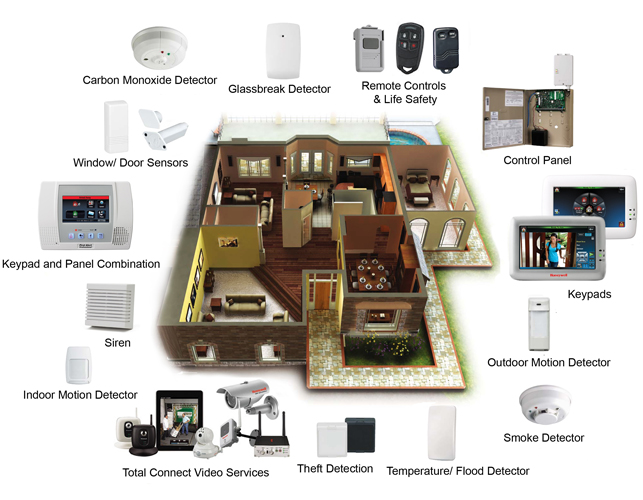
\includegraphics[width=0.9\textwidth]{images/Chapter_02/security.jpg}
	\caption{Example of a smart home with security-oriented devices}
	\label{fig:security-in-smarthome}
\end{figure}

\bigskip
There is not an exact point where we can set the beginning of the domotics as a real concept, but during the last century
there has been some remarkable efforts, and even before. In 1898, Nikola Tesla created a wireless control for a toy boat, 
the first of its kind \cite{betanewsHistory}. That marks the beginning of wireless technologies, one of the fundamental
parts of Home Automation. 

\bigskip
In 1975, after lots of appearances of the idea of home automation in films, the first general purpose home automation
technology, called X10, was developed. X10 defines a protocol for communication between electrical devices, which uses power
line wiring for signaling and control, where the signals involve brief radio frequency bursts representing digital information.
Therefore, it also defines a wireless radio based protocol. Surprisingly, the X10 technology is still widely used and available,
with millions of units in use worldwide.

\bigskip
However, it was not until 1984 that the word Smart Home appeared, invented by the \textit{American Association of House
Builders}. After that, different inventions rapidly followed one another, with devices such as\\ \textit{The Clapper} (which 
was operated through sound, like a clap or a bark) and interest from the biggest technological companies, like Microsoft.

\begin{figure}
	\centering
	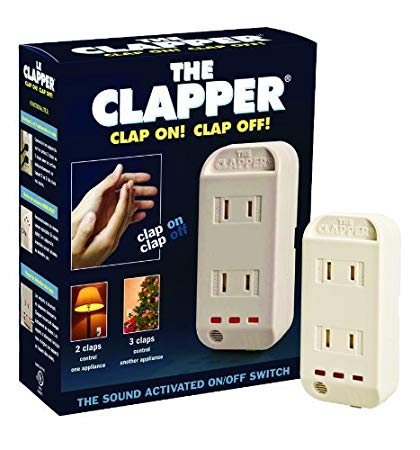
\includegraphics[width=0.5\textwidth]{images/Chapter_02/the-clapper.jpg}
	\caption{The Clapper, a sound-activated switch}
	\label{fig:the-clapper}
\end{figure}

\bigskip
Home Automation has not stopped gaining ground on our homes and now it is experiencing one of the best moments
in its lifetime, with the unstoppable growth of the Internet of Things (IoT) and the simultaneous development of Artificial 
Intelligence for the general public, with the biggest companies, like Google and Apple, investing millions of dollars on it.
Devices like Amazon Echo and Google Home, or assistants like Siri, Cortana, Google Assistant and Amazon Alexa are a 
good representative of this trend. I will talk in depth about them in the following sections.

\bigskip
We have always imagined that Smart Homes would bring us a whole world of benefits. And that is partly true, but
they have ended up offering benefits that no one could imagine some decades before, when matters such as energy
savings were not as important as today. These benefits are responsible for their increasing popularity, and they can be 
summarized in the following points:

\begin{itemize}
	\item \textbf{Control anywhere:} Smart Homes can be completely controlled anywhere in the world from smart phones or
	other devices with Internet connection, so we can know the status of our devices at any time. That would allow us, for
	example, to stop worrying when staging out of home thinking if we have left the air conditioning on.
	\item \textbf{Safety:} there are tons of security systems ready to work on Smart Houses. They are capable of monitoring
	the people going in and out of home and send alerts to the owners if necessary. Like many other devices, there are also
	smart locks for the door and cameras that we can control from our smart device.
	\item \textbf{Accessibility:} Smart Homes can increase a lot the quality of life of elderly or disabled people, as they can be
	managed via voice commands, making the interaction much easier to people which is not experienced with computers and
	improving their independence.
	\item \textbf{Energy efficiency:} one of the main goals of Home Automation is to work with the least amount of energy 
	needed, and a big part of the research in this field is going in this direction. There are induction cook-top stoves that can be 
	powered on only if there is anything placed over them (and even get the perfect cooking, powering off themselves)\cite{directenergyAdvantages}
	or heating systems that power on and off depending on the weather and inner conditions of the home, or even a faucet 
	technology that can maximize shower water usage by shaping the individual droplets of water, so the experience feels 
	almost the same but with less water usage. 
	\item \textbf{Money saving:} the last point leads to another benefit: saving money. Smart Homes can use less energy and 
	water, making a big difference in how much we pay at the end of the month. Reports show that the savings on the energy bill 
	for this reason range from 10\% to 30\%.\cite{directenergyAdvantages}
	\item \textbf{Comfort:} Smart Houses can also help save time. Today, when everyone is trying to make the most of their free
	time, this technology is capable of doing housework, so that people can spend their time on things they enjoy most, or simply 
	gain time  to spend with their families.
\end{itemize}

\bigskip
This range of benefits has made possible to see home automation systems in many homes, but also in offices. Now, almost 
every new house that is built is prepared for domotics, including Internet access points in every room, a big amount of plugs, 
and a lot of space to extend its capabilities in a future. Indeed, the global home automation and security control market is 
expected to reach 12.81 billion dollars by 2020.\cite{reutersResearchMarkets} The following charts is a perfect example of how 
rapidly is growing the Smart Home sector and how powerful it is at this moment, showing the data for the most important Smart
Home market at this moment: the United States.

\begin{figure}
	\centering
	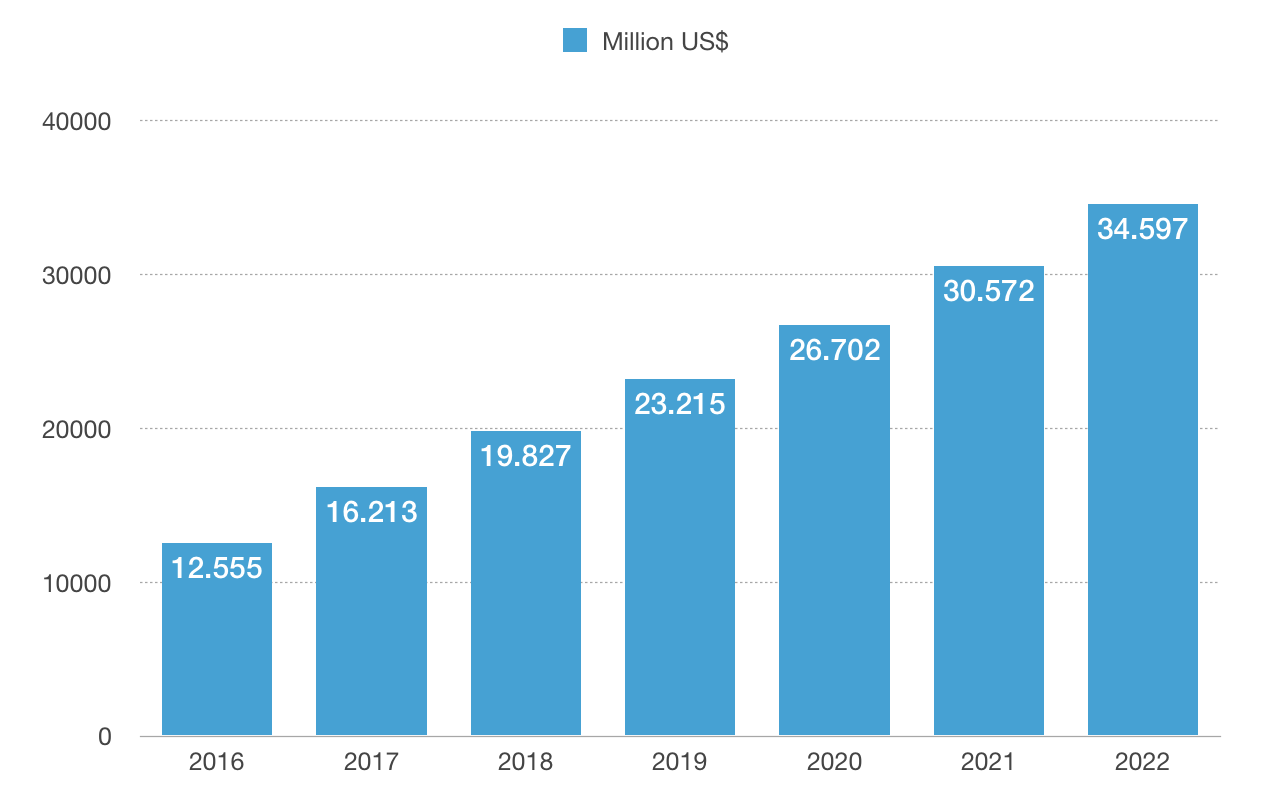
\includegraphics[width=0.9\textwidth]{images/Chapter_02/sh-market-revenue.png}
	\caption{The Smart Home Market revenue from 2016 to 2022 in the US\cite{statistaSmartHomeUS}}
	\label{fig:sh-market-revenue}
\end{figure}

\bigskip
Predictions are not bad either: they show that this trend will continue in the coming years, reaching 34.5 million of the 
US dollars, and this is just in the United States, although there will be similar situations in the rest of the world.

\section{Home Automation System Design}
After a look at the definition and history of Home Automation and its benefits, I am going to explain how these systems are 
usually organized. There is more than one valid way, and it will always depend on the requirements and conditions of the user,
the home environment and of course the capabilities of its components. The figure \ref{fig:sh-basic-structure} is a good 
example of a basic organization for Home Automation\cite{embeddedHASystemDesign}. This organization has a name, indeed:
centralized architecture.

\begin{figure}
	\centering
	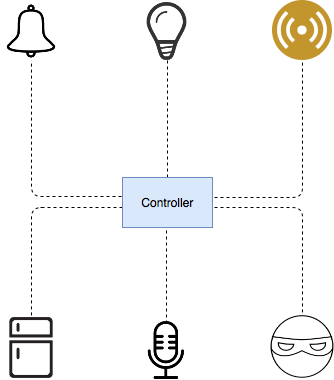
\includegraphics[width=0.55\textwidth]{images/Chapter_02/basic-sh-structure.png}
	\caption{Centralized Smart Home structure}
	\label{fig:sh-basic-structure}
\end{figure}

\subsection{Centralized Architecture}
In a centralized Smart Home Environment architecture, the Control System, which is realized by means of a computer
system, is in charge of acquiring data from sensors, providing a user interface, and executing the control algorithms and 
sending instructions to actuators.\cite{badica13} In the example in the figure \ref{fig:sh-basic-structure}, the sensor (in gold) 
can represent a smoke detector that can trigger the alarm (the actuator) to alert the householders.

\bigskip
The controller is often called Home Gateway, and in this case it is the central computer. It is also responsible of making 
accessible the system via Internet, as well as providing services to the home residents. An option to increase its performance 
while maintaining the same architecture is to limit the functionalities of the Home Gateway to data acquisition, software 
interfacing with domotic devices and basic processing, and to delegate to more powerful servers outside home the most
part of the processing.

\bigskip
This is the most popular architecture in home automation, partly because product manufacturers tend to centralize communications
between their intelligent devices in a hub or gateway of the same brand, which users need to install to operate the rest of the devices.

\subsection{Distributed Architecture}
In a distributed Smart Home Environment architecture, the Control System software is conceptualized and implemented as a 
distributed computing system, that is, a series of intercommunicating computers working together to achieve an end, which in this 
case is running a Smart Home system.

\bigskip
The distributed architecture benefits from the computational resources of smart devices to integrate software components into the 
nodes of the Home Automation network, which produces a big increase in performance and modularity. However, the cost of 
this architecture is significantly higher compared to the centralized architecture, and therefore it is hard to achieve a big degree of
granularity. For this reason, this architecture is often applied conceptually, while still physically centralized into the Home Gateway.





\chapter{Voice Assistance}

We spend so much time using devices that have integrated voice assistants that we usually forget how incredibly fast they have
evolved. Nowadays, they can recognize thousands of words and expressions really fast, and they are even capable to imitate
emotions. What is more, they fit in a pocket. But the reality was totally different just a couple of decades ago. From the IBM
Shoebox to Siri, in this chapter I will explore the fundamentals of voice assistance.

\section{What is Voice Assistance?}
Voice assistance is the result of another form of interaction between humans and computers.\cite{botsocietyVUI} The Voice User
Interface (VUI), which has the voice assistants as a result, allows a user to interact with computer or mobile or other electronic 
devices through speech or voice commands. Thus, VUI is an interface of any speech recognition applications.

Therefore, a voice assistance, also known as virtual assistant, is an application program that understands natural language voice 
commands and can perform tasks or services for an individual. Its expansion has been truly remarkable in the last few years, to the
point that we can see devices that exclusively work as virtual assistants, with integration with many other services. Its real usefulness
in society, though, remains to be seen, as this field is commonly viewed with skepticism and mistrust, and the fact of talking to a 
machine as if it were another human being remains an obstacle to overcome.

As I mentioned, voice assistants are now present in plenty of platforms:
\begin{itemize}
	\item \textbf{Smart speakers:} Google Home (Fig. \ref{fig:google-home}), Apple HomePod, Amazon Echo, Movistar Home.
	\item \textbf{Mobile operating systems:} Siri on iOS, Google Assistant on Android, Bixby on Samsung phones.
	\item \textbf{Desktop operating systems:} Siri on macOS and Cortana on Windows 10.
	\item \textbf{Smartwatches}: Apple Watch, Google Wear OS.
	\item \textbf{Cars:} Apple CarPlay, Android Auto. 
	\item \textbf{Televisions:} Siri on Apple TV (Fig. \ref{fig:apple-tv}) and the voice assistant in Samsung Smart TVs.
	\item \textbf{Inside mobile apps:} EVO Assistant in the mobile application of the Spanish bank EVO.
\end{itemize}

\begin{figure}
	\centering
	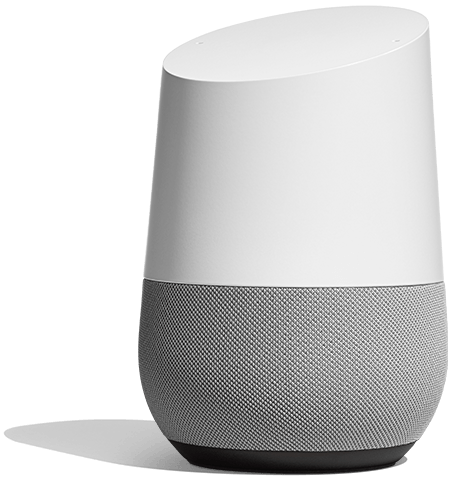
\includegraphics[width=0.5\textwidth]{images/Chapter_03/google-home.png}
	\caption{Google Home, a smart speaker integrated with the Google Assistant}
	\label{fig:google-home}
\end{figure}

\begin{figure}
	\centering
	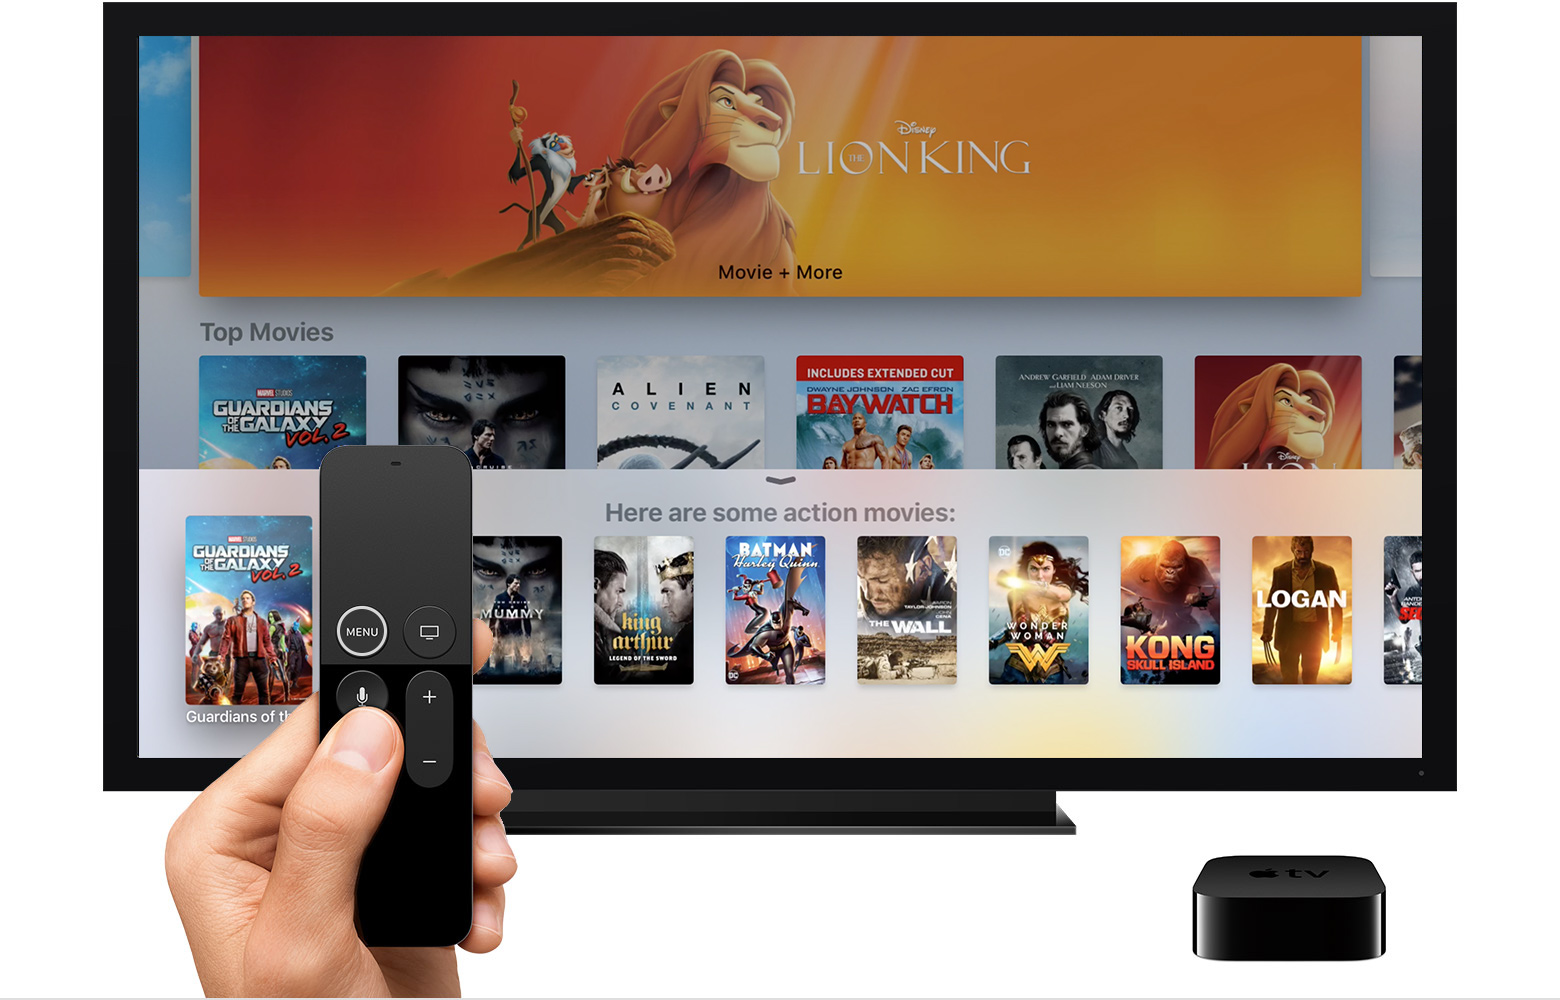
\includegraphics[width=0.9\textwidth]{images/Chapter_03/apple-tv.jpg}
	\caption{Apple TV and the Siri Remote, which has a microphone to interact with the assistant}
	\label{fig:apple-tv}
\end{figure}

The history of voice assistance goes back to 1961, when IBM introduced the IBM Shoebox.\cite{voicebotTimeline} 
This was a very innovative product at that moment. Although it was not suitable for commercial use, it did mark the 
beginning of a revolution, the fruits of which we can now see. 

The Shoebox was capable of recognizing 16 spoken words, including ten digits from 0 through 9. When a number and 
command words such as \textit{plus}, \textit{minus} and \textit{total} were spoken, Shoebox instructed an adding machine 
to calculate and print answers to simple arithmetic problems. It classified the electrical impulses generated from a microphone
according to various types of sounds and activated the attached adding machine through a relay system.\cite{ibmArchivesShoebox}

Later on, there were more attempts from the research field, as the HARPY Speech Recognition System from the Carnegie
Mellon University, in 1976.\cite{lowerre76} Is could recognize about 1000 words.

Nevertheless, it was not until 1990 that the first speech recognition for consumers appeared: the Dragon Dictate. Seven years
later, the same company presented the Dragon NaturallySpeaking, which introduced continuous speech recognition as a novelty.
They led the way with competent voice recognition and transcription. This field attracted the attention from big companies of that 
time, and Microsoft began working on their own assistant: Clippy, in the Microsoft Office suite. In spite of the fact that this was 
not a voice assistant exactly, it showed how natural language could be interpreted and used in order to allow the human-computer
interaction. It was quite unpopular and Microsoft decided to end it on 2001, but its impact was huge for the assistants that followed
it. A bit before Windows XP, Microsoft introduced the speech recognition feature in their Office XP suite.

With the launch of Siri in 2014, Apple marked the modern era of voice assistants. For the first time, people could fit a full functional
voice assistant in their pocket. And most importantly, Siri reached a wide audience and began to popularize this technology.
Siri was able to make searches on Internet and reproduce the results, to set reminders and events in the calendar or to call any
contact by its name, between many others. In addition, it included a layer of \textit{natural interaction} with the user, being able to 
respond to any other phrase as any other human would (even to sentences that were not commands, like \textit{How do you feel 
today?} or \textit{Tell me a joke}).

Google, with Google Now, and then Microsoft and Amazon, with Cortana and Alexa respectively, followed this trend, even improving
on what Siri failed, and in the case of Microsoft, making a voice assistant available on PCs as well. Then, in 2014, Amazon introduced
Echo, the first smart speaker of all time. It was just the beginning of what we now call the \textit{Smart Speaker Revolution}.\cite{voicebotTimeline}

After the Echo, Apple and Google followed with the HomePod and Home, respectively. In fact, Google Home has been recently
launched in Spain, and the HomePod is not available yet, as an example of how recent this technology is. Its number of users is 
expected to continue to grow, and even faster than it has already done.\cite{statistaDigitalAssistants}

\begin{figure}
	\centering
	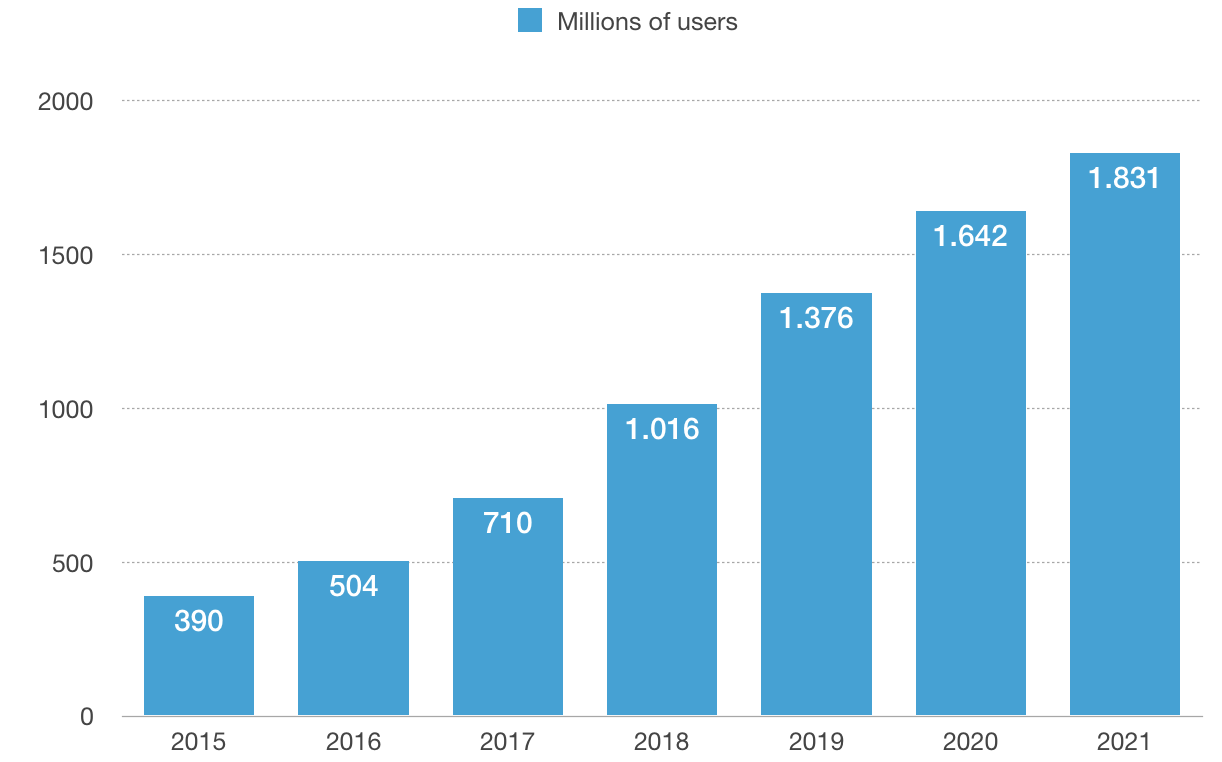
\includegraphics[width=0.9\textwidth]{images/Chapter_03/voice-assistants-usage.png}
	\caption{Estimated number of users of virtual assistants worldwide \cite{statistaDigitalAssistants}}
	\label{fig:voice-assistants-usage}
\end{figure}

\bigskip
\section{Services Voice Assistants Provide}
The range of services provided by voice assistants is constantly becoming bigger, as they are a booming technology that is constantly
receiving new updates. The following are shared by most of the virtual assistants currently:
\begin{itemize}
	\item Provide information, such as weather forecast, routes to any point in a map or general knowledge.
	\item Manage components in a Home Automation environment.
	\item Interact with media content, such as music and video (which is commonly integrated with streaming services, like Netfix or 
	Apple Music).
	\item Make phone calls and send instant messages.
	\item Manage the personal agenda.
	\item Provide accessibility indications.
	\item In call centers, they complement or replace the customer service by humans.
\end{itemize}

We are nowadays in the first stages of this new technology, that combines artificial intelligence, machine learning, voice recognition 
and human-computer interaction. Google is the company that apparently has done the biggest advancements and, in fact, they have 
recently introduced Google Duplex, a technology capable of almost perfectly simulating a human speech, which can be used for a wide
range of purposes, such as ordering food or making an appointment with a hairdresser. This would be a new service to include in 
the previous list.

They are also providing very useful tools to developers and makers, like the Cloud Speech-To-Text API. I will come back to this 
technology in the following chapters, as it will be an essential part to achieve my objective, the creation of a voice-driven home 
automation controller, a service that can also be seen in the previous list.



\chapter{Product Analysis}

The aim of this chapter is to provide a detailed analysis of the devices more closely related to this project, now that we have a
clearer idea about its main pillars. I will go into many of the available commercial devices and software in the fields of home
automation, voice assistance and smart devices.

\section{Home Automation Systems}
This section covers all the hardware and software systems related to home automation. As we will see, there are lots of solutions
with very different purposes: while there is Amazon Alexa, a full hardware and software system that integrates other home automation
systems, we can also find pure online solutions, like the automation platform IFTTT. Sometimes, home automation systems are
built underneath a virtual assistant, as it happens with Amazon Alexa, so some devices are going to appear in this section and in the
next one. However, they will analyzed from two different perspectives, as having a good virtual assistant does not mean having a
good home automation system.

\subsection{Philips Hue}
Philips Hue is a personal wireless lighting system aimed at the smart home. In combines LED light bulbs, LED strips and other
lighting devices, and sensors that can be configured in their mobile app, so they can modify the home lighting based on a set of
rules. There is a wide range of products, including color and only white lights, so users can build a pretty customizable lighting
experience.\cite{philipsHueMeethue}

The system requires a bridge connected to the Internet (called Philips Hue Smart Hub) in order to work. This is because the Hue
devices do not use WiFi in order to communicate with the bridge, but the system needs to have WiFi to be controllable from a
mobile phone. Thus, it follows a centralized architecture. Moreover, Philips does not provide any type of assistant or external interface
to manage the system apart from the mobile application by default, although Hue works with the most popular home automation
systems, like Alexa or Apple HomeKit, that provide much more flexible home automation management.

\begin{figure}
	\centering
	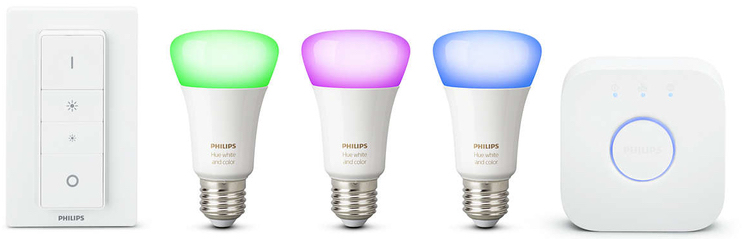
\includegraphics[width=0.9\textwidth]{images/Chapter_04/philips-hue.jpg}
	\caption{A Philips Hue dimmer switch, three color light bulbs and the Hue Smart Hub}
	\label{fig:philips-hue}
\end{figure}

\subsection{LG SmartThinQ}
LG SmartThinQ groups the range of Wi-Fi enabled home appliances made by the company LG, including refrigerators, dishwashers,
vacuum cleaners or air purifiers, between others. As of September 2017, they were the most extensive range of devices of their
kind.\cite{lgSmartThinq}

Unlike Philips Hue, SmartThinQ devices do not require a bridge to work. They can be controlled from the mobile phone and, in some
cases, like in the refrigerators, they include a touchscreen to interact with the device. However, LG does not provide any extra device
or virtual assistant to interact with them, though they are manageable through Amazon Alexa and Google Assistant. A standard setup
with this system will follow a hybrid architecture, as some devices are also their controllers, but there can also be external controllers.

\subsection{Samsung SmartThings}
Samsung SmartThings is a home automation system composed by a series of applications for the Samsung mobile phones, Samsung
TVs and Samung refrigerators. It is even possible to do small management tasks from Samsung smartwatches, called Galaxy Gear. It
uses the cloud to synchronize all the applications, in order to have the most recent information in all of them. This makes it necessary
for the user to have a Samsung account.\cite{samsungSmartthings}

Unlike the previous systems, SmartThings is not a specific system for a range of devices from the same maker, but it is more aimed
to provide an effective interconnection between devices from different makers, as long as they are compatible with their system.
The SmartThings Smart Home Hub is necessary in order to use Samsung SmartThings. It is a bridge that supports common home
automation protocols, like Zigbee or Z-wave, essential to manage some devices that only use these protocols. It also provides
comprehensive automation options.\cite{smartHomeBeginner} The usage of the Hub makes the architecture of this system centralized.

Furthermore, SmartThings is not yet compatible with many commercial devices, and the restrictions imposed by Samsung forces the
user to stick to their environment. In addition, the system is not open source, so making any modification apart from the ones that
Samsung allows is impossible. Also, users are forced to purchase the Smart Home Hub, which makes it necessary to have an additional
device, unlike other similar systems. The system is compatible with Bixby, the virtual assistant from Samsung.

\subsection{Google Home}
Introduced at Google I/O 2016, the annual Google developer conference, \textit{Google Home} is the name of Google's smart speaker,
which is Google's biggest insight into home automation technology. Its aim is to work with all the possible smart home devices, so it
follows the same idea as the Samsung SmartThings system, being a \textit{maker-independent} system, as long as, of course, devices
are compatible with it. Also, Google Home brings all the functions of Google Assistant to the smart speaker.

The main difference with SmartThings is that this system is mainly voice-driven. The home automation layer is pushed down to just
one more function of the virtual assistant, and Google does not even provide a graphical interface to manage the smart devices.
Anyway, normally the makers of each device provide a mobile application from where users can manage their devices in a more
user-friendly interface, but having a centralized view is a desirable feature. On the bright side, all Google devices that support
Google Assistant can automatically control smart home devices.

The number of compatible devices with the Google Assistant, unlike SmartThings, is very high, and almost any new smart home
device is tagged as compatible with it.

\subsection{Apple HomeKit}
HomeKit is the result of Apple's efforts to create a home automation environment adapted to its devices. It has been also made to work
with a wide range of devices, but in this case, Apple included some notable security policies, with the goal of achieving the highest
security and privacy. In fact, all HomeKit devices need to be approved by Apple first.

On iPhone and Mac computers (starting with macOS Mojave), Apple includes an application called Home, which displays all
of the smart home devices in a convenient way and lets people organize and manage them. In addition, it is also possible to establish
automation rules, based on the user's location, time of day, actions or even occupancy of the house. Furthermore, Apple also provides
integration with their personal assistant, Siri. As it happens with the Google Assistant, all Apple devices configured with the same Apple
ID will have the same information automatically synchronized.\cite{appleIOSHome} Usually, systems made under Apple HomeKit will follow
a decentralized architecture.

Although this is a very comprehensive home automation system, the number of compatible devices is not as high as in other options.
Apple has been lately working on promoting their home automation system and their assistant by introducing the HomePod, their smart
speaker with Siri.

\subsection{Somfy}
Somfy is a French company founded in 1960, which since the 1980s has been devoted to the construction of home automation systems.
They have implemented their solutions in important places, like the United Nations Headquarters or the Vancouver Convention Center
and have created their own home automation technologies, such as \textit{Radio Technology Somfy (RTS)} and \textit{Somfy Digital
Network (SDN)}.\cite{somfyOurStory}

Their range of products goes from control devices (as hand-held remotes, mobile applications and wireless switches) and sensors (sunlight,
temperature, wind) to blinds, lighting systems and other smart home utilities. Unfortunately, the control devices only work with Somfy
devices. The system follows a hybrid architecture, where each device is a controller, but there can also be extra controllers, like the
hand-held remotes.
\\~\\

In addition to the previous domotic systems, which are proprietary, there are also open source and more customizable solutions that,
although they may require more time in their configuration, are much more adaptable to the needs of the user. I will explore three of
the most popular: openHAB, Home-Assistant.io and Jeedom.

\subsection{OpenHAB}
OpenHAB, the acronym for Open Home Automation Bus is an open source, technology agnostic home automation platform which runs
as the center of the smart home. \cite{openHABDocs} This means that its aim is to integrate different home automation systems into
a single one. It allows the user to configure almost every aspect of the system, providing a common interface and a uniform approach
to automation rules.

In its most recent version, openHAB 2, it has implemented new user interfaces that automate many processes, so it is almost unnecessary
to write a single line of code, making the system more attractive to all types of users. OpenHAB needs to be installed in a computer that
will act as a server in the local network, making the system accessible via HTTP. It also offers more connectivity options that I will explore
in the following chapters. The architecture, in this case, is decentralized, as there may be multiple controllers, including openHAB itself.

OpenHAB's compatibility is somewhat limited when it comes to home automation devices, but it supports Apple HomeKit and common
protocols, such as ZigBee and Z-Wave, to get rid of specific gateways from other systems.\cite{openHABAddons}

\subsection{Home-Assistant.io}
Home-Assistant.io, or simply Home Assistant, is a open source home automation platform running on Python 3.\cite{homeAssistantio}
Based on a distribution called \textit{Hass.io}, it creates a secured local server in the computer where it is installed. It is accessible via
HTTP and also includes a web user interface that will automate the process of discovering and configuring devices. In terms of
functionality, it is very similar to openHAB, although it might be a little simpler for some users, as it uses the YAML syntax for
configuration, while openHAB has its own.

Its functionality is organized in \textit{Components}, the name that Home Assistant gives to any add-on, which will add a compatibility
layer with a device, system or service. They are fully backed by the Home Assistant community and they are similar in number and type to
what openHAB provides, but with very interesting additions, including Wink and Arduino.

\begin{figure}
	\centering
	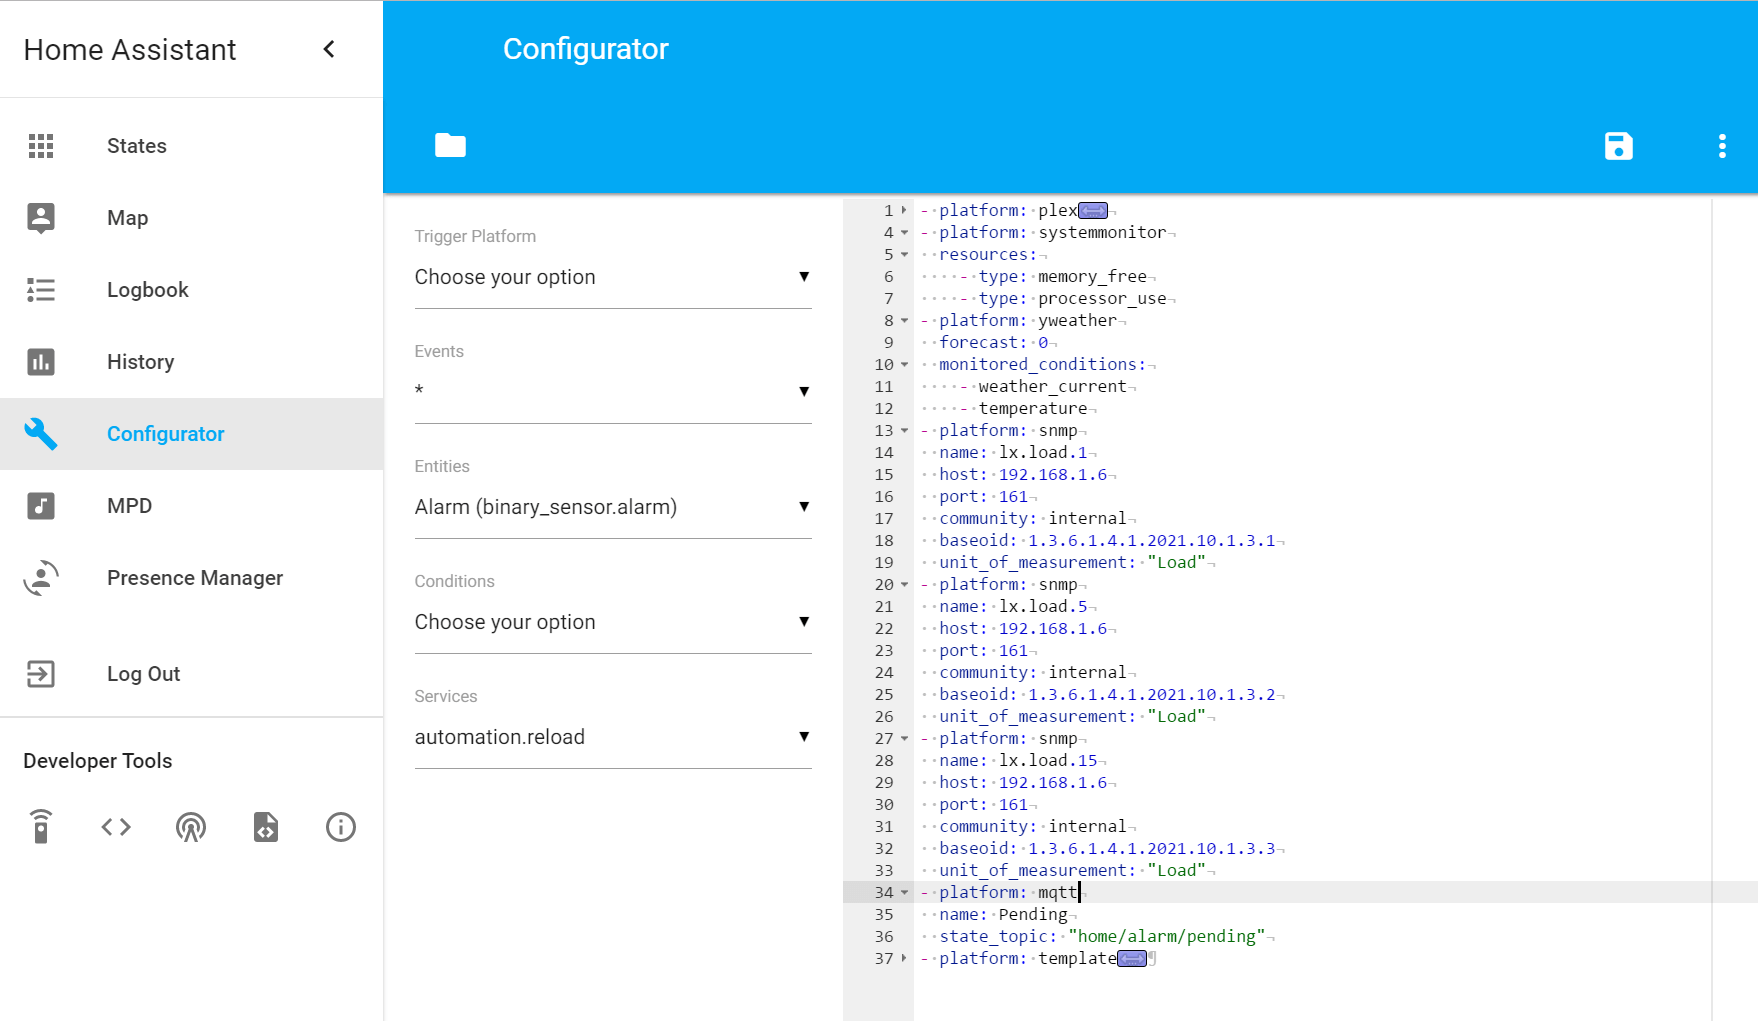
\includegraphics[width=0.95\textwidth]{images/Chapter_04/home-assistant-configuration.png}
	\caption{Home-Assistant.io web user interface}
	\label{fig:home-assistant-configuration}
\end{figure}

\subsection{Jeedom}
Jeedom is a open source, multi-protocol, autonomous and customizable home automation software.\cite{jeedomDoc} It is aimed for
individuals and professionals, and provides custom support for both. They also sell what they call \textit{Boxes}, which are small
computers with Jeedom pre-installed, although their software can be installed on any Linux system. Jeedom also provides mobile phone
apps for Android and iOS, which connect to the Jeedom system by scanning a QR code. As in the previous platforms, they also provide
the \textit{Jeedom Market}, from where users can add new features to their system.

Also, there are different Jeedom versions, which are called \textit{Service packs}. There is the free and open source version, which
includes the lowest number of functionalities. Then, the other versions can be purchased, although some of them come with their Boxes,
and they include dynamic DNS and HTTPS, the mobile application for free or more plugins offered, among other things.

Although the free version is fully open source, the limitations that it has and the obligation to pay in order to have the \textit{full
experience}, could annoy some users and make them lean towards other platforms.
\\~\\

It seems difficult to directly compare these home automation systems, but all of them share characteristics that we can contrast.
The table \ref{table:home-automation-comparison} represents a comparison of the features that I consider most important.

\begin{sidewaystable}[]
	\begin{center}
		\resizebox{\textwidth}{!}{
		\begin{tabular}{|p{0.1\linewidth}|p{0.15\linewidth}|p{0.05\linewidth}|p{0.05\linewidth}|p{0.15\linewidth}|p{0.15\linewidth}|p{0.1\linewidth}|p{0.1\linewidth}|p{0.39\linewidth}|}
			\hline
			\textbf{System name} & \textbf{Developer}                                    & \textbf{Free} & \textbf{Open source} & \textbf{Architecture} & \textbf{Requirements}                               & \textbf{Extra software}                                        & \textbf{Extra hardware}               & \textbf{Compatibility}                                                                                          \\ \hline
			Hue                  & Philips                                               & No                     & No                   & Centralized           & Hue Smart Hub                                       & Mobile app                                                     & Hue devices                           & \begin{tabular}[l]{@{}l@{}}Only for Hue devices\\ Integrable in Alexa, Google Assistant, HomeKit\end{tabular}   \\ \hline
			SmartThinQ           & LG                                                    & No                     & No                   & Hybrid                & None                                                & Mobile app                                                     & SmartThinQ devices                    & \begin{tabular}[l]{@{}l@{}}Only for SmartThinQ devices \\ Integrable in Alexa and Google Assistant\end{tabular} \\ \hline
			SmartThings          & Samsung                                               & No                     & No                   & Centralized           & Smart Home Hub                                      & Mobile app                                                     & Samsung smart home devices            & \begin{tabular}[l]{@{}l@{}}Compatible with devices from different makers\\ Integrated in Bixby\end{tabular}     \\ \hline
			Assistant            & Google                                                & No                     & No                   & Centralized           & A device with Google Assistant                      & Google Home app                                                & Google Home smart speaker             & Huge compatibility with devices from different makers                                                           \\ \hline
			HomeKit              & Apple                                                 & No                     & No                   & Decentralized         & An Apple device                                     & Home app                                                       & Apple HomePod                         & \begin{tabular}[l]{@{}l@{}}Compatible with devices from different makers\\ Integrated in Siri\end{tabular}      \\ \hline
			Somfy                & Somfy                                                 & No                     & No                   & Hybrid                & None                                                & Mobile app                                                     & Somfy smart home devices and controls & Only for Somfy devices                                                                                          \\ \hline
			openHAB              & The openHAB Community and the openHAB Foundation e.V. & Yes                    & Yes                  & Decentralized         & A computer with Internet connection                 & \begin{tabular}[l]{@{}l@{}}myopenHAB\\ openHABian\end{tabular} & None                                  & Compatible with devices and services from different makers, fully customizable                                  \\ \hline
			Home Assistant       & The Home Assistant community                          & Yes                    & Yes                  & Decentralized         & A computer with Internet connection                 & \begin{tabular}[l]{@{}l@{}}iOS app\\ Hass.io\end{tabular}      & None                                  & Compatible with devices and services from different makers, fully customizable                                  \\ \hline
			Jeedom               & Jeedom SAS                                            & Partly             & Partly           & Decentralized         & A computer with Internet connection or a Jeedom Box & Mobile app                                                     & Jeedom Boxes                          & Compatible with devices and services from different makers                                                      \\ \hline
		\end{tabular}}
		\caption{Comparison between different home automation systems}
		\label{table:home-automation-comparison}
	\end{center}
\end{sidewaystable}

\bigskip
\section{Home Automation Devices and Related Services}
In this section I will explore different devices, services and protocols that may be suitable for the outcome of this project.
The section presents a brief description of each device and a comparison between the same type of devices. These devices are
usually handled in the same way in open source home automation systems. For example, in openHAB they are called 
bindings\cite{openHABDocs}, and each of them is installable over the base system. As the main idea is to use open source technologies 
in this project, I will focus on compatible devices, and analyze them based on their integration with openHAB. Therefore, I will talk about 
bindings, which is the abstraction layer that openHAB employs for devices, services and protocols.

\subsection{Alarms}

\subsubsection{DSC PowerSeries Alarm System}
The DSC PowerSeries Alarm System is a popular do-it-yourself home security system, which can be monitored and controlled remotely
through a standard web-browser or mobile device.\\~\\
Pros:
\begin{itemize}
	\item Supporting a DIY Alarm System is acceptable due to the range of users we expect to cover
	\item Communication via API (OpenHAB binding)
\end{itemize}
Cons:
\begin{itemize}
	\item Availability of this product outside USA
\end{itemize}

\subsection{Amazon Dash Button}
The Amazon Dash Button is a cheap and small Wi-Fi connected device to order products from Amazon with the simple press of
a button. This Binding allows to integrate Dash Buttons into the controller.\\~\\
What to consider:
\begin{itemize}
	\item Privacy concern: The Dash Button will try to contact the Amazon servers every time the button is pressed. Details about
	this can be read in this section of the documentation.
	\item The Binding uses Pcap4J in order to capture ARP and BOOTP requests send by the Amazon Dash Button. Buttons will
	hence only be usable within the same network as your openHAB instance.
\end{itemize}
Pros:
\begin{itemize}
	\item Usability
	\item Communication via API (OpenHAB binding)
	\item Easy to configure
\end{itemize}
Cons:
\begin{itemize}
	\item Not open source
	\item Manual device addition
\end{itemize}

\subsection{AV Receivers}

\subsubsection{Denon}
The openHAB Denon Binding allows interaction with Denon AV receivers.\\~\\
Pros:
\begin{itemize}
	\item Plenty of available settings
	\item Communication via API (OpenHAB binding)
\end{itemize}
Cons:
\begin{itemize}
	\item Not a common device
	\item Manual device addition
\end{itemize}

\subsubsection{Marantz}
Denon binding also seem to work with Marantz devices.

\subsubsection{Onkyo}
This binding integrates the Onkyo AV receivers. Binding should be compatible with Onkyo
AV receivers which support ISCP (Integra Serial Control Protocol) over Ethernet (eISCP).\\~\\
Pros:
\begin{itemize}
	\item Communication via API (OpenHAB binding)
	\item Usually cheaper than Denon devices
\end{itemize}
Cons:
\begin{itemize}
	\item Quite limited product support
\end{itemize}

\subsection{Digital Media Players}

\subsubsection{Google Chromecast}
The binding integrates Google Chromecast streaming devices.
It not only acts as a typical binding, but also registers each Chromecast device as an audio sink that can be used for playback.

The binding currently supports the “classic” Chromecast that is an HDMI dongle as well as the Chromecast Audio, which only does
 audio streaming and offers a headphone jack.

Chromecast devices are discovered on the network using UPnP. No authentication is required for accessing the devices on the network.
They can also be manually added.\\~\\
Pros:
\begin{itemize}
	\item Common device
	\item Automatic discovery
	\item Communication via API (OpenHAB binding)
\end{itemize}
Cons:
\begin{itemize}
	\item Not many actions can be performed
	\item Current library might be problematic because of how it works
\end{itemize}

\subsubsection{Kodi}
Kodi is a free and open source software media center for playing videos, music, pictures, games, and more. Kodi runs on Linux, OS X,
BSD, Windows, iOS, and Android. It allows users to play and view most videos, music, podcasts, and other digital media files from local
and network storage media and the internet.
The Kodi Binding integrated Kodi media center support with openHAB, allowing both controlling the player as well as retrieving player
status data like the currently played movie title.\\~\\
What to consider:
\begin{itemize}
	\item Needs some initial configuration in Kodi.
\end{itemize}
Pros:
\begin{itemize}
	\item Auto-discovery feature
	\item Fully open source
	\item Extremely cheap and useful solution, capable of running in almost every device
	\item Communication via API (OpenHAB binding)
\end{itemize}

\subsubsection{Plex}
This binding supports multiple clients connected to a Plex Media Server. With this binding, it’s possible to dim the lights when a video
starts playing, for example.
Most changes are pushed to the binding using web sockets. Polling (and the corresponding refresh interval) is only applicable to the
online/offline status of clients.\\~\\
What to consider:
\begin{itemize}
	\item It is necessary to configure the username and password (or to use the Plex token) in order to make it work.
\end{itemize}
Pros:
\begin{itemize}
	\item Plex is a free and easy to use media centre, available for many platforms
	\item Wide control of the Plex Media Server from OpenHAB
	\item Communication via API (OpenHAB binding)
\end{itemize}
Cons:
\begin{itemize}
	\item Plex is not fully open source
\end{itemize}

\subsection{Garage Door Control}

\subsubsection{Chamberlain MyQ}
Chamberlain MyQ system allows you to connect the garage door to the internet to be controlled from anywhere using a smartphone. Using
this API, The Chamberlain MyQ Binding can get the status of the garage door opener and send commands to open or close it.\\~\\
Pros:
\begin{itemize}
	\item Easy to control, only needs the user and password to start working
	\item Communication via API (OpenHAB binding)
	\item Availability in Europe
\end{itemize}
Cons:
\begin{itemize}
	\item High price (Starting at EUR 200, Amazon Spain price)
\end{itemize}

\subsection{Garden Care}

\subsubsection{Gardena}
This binding allows to integrate, view and control Gardena Smart Home devices in the openHAB environment.\\~\\
Pros:
\begin{itemize}
	\item There are not many smart solutions for garden care, but Gardena can fulfil any needs
	\item Communication via API (OpenHAB binding)
\end{itemize}
Cons:
\begin{itemize}
	\item Needs an account to discover the devices, though the discovery is fully automatic once the account is set
\end{itemize}

\subsection{Lighting}

\subsubsection{Philips Hue Lighting System}
This binding integrates the Philips Hue Lighting system. The integration happens through the Hue bridge, which
acts as an IP gateway to the ZigBee devices.\\~\\
What to consider:
\begin{itemize}
	\item The Hue Smart Bridge is required.
	\item Almost all available Hue devices are supported by this binding. This includes not only the “friends of Hue”,
	but also products like the LivingWhites adapter.
	\item Devices need to be registered with the Hue bridge before it is possible for this binding to use them.
	\item The Hue bridge is discovered through UPnP in the local network. Once it is added as a Thing, its authentication
	button (in the middle) needs to be pressed in order to authorize the binding to access it. Once the binding is authorized,
	it automatically reads all devices that are set up on the Hue bridge and puts them in the Inbox
\end{itemize}
Pros:
\begin{itemize}
	\item Philps Hue is a beautiful and easy way to take advantage of home automation and smart devices. Its devices are very
	common and useful, being the final user its main target
	\item Compatibility with many other systems (Alexa, Apple HomeKit, etc.)
	\item Communication via API (OpenHAB binding)
\end{itemize}
Cons:
\begin{itemize}
	\item Need an extra device (the Hue Smart Bridge) to communicate with the rest of them
\end{itemize}

\subsubsection{LIFX LED Lightning}
This binding integrates the LIFX LED Lights. All LIFX lights are directly connected to the WLAN and the binding communicates with
them over a UDP protocol.\\~\\
What to consider:
\begin{itemize}
	\item The binding is able to auto-discover all lights in a network over the LIFX UDP protocol. Therefore, all lights must be turned on
\end{itemize}
Pros:
\begin{itemize}
	\item LIFX is one of the most popular alternatives to Philips Hue
	\item No need of any extra device
	\item Communication via API (OpenHAB binding)
\end{itemize}
Cons:
\begin{itemize}
	\item More expensive that Philips Hue (EUR 65 vs. EUR 45, Amazon Spain prices)
	\item Less compatibility than Philips Hue
\end{itemize}

\subsubsection{MiLight, EasyBulb, Limitless LED and iBox}
This binding is for using Milight, Easybulb or LimitlessLed bulbs and the iBox.\\~\\
What to consider:
\begin{itemize}
	\item The binding supports Milight/Easybulb bridges from 2014+, iBox from 2016 and iBox2 from 2017 and their respective bulbs.
	The Dual White bulbs from 2015 and the new generation of Dual White bulbs is supported. RGB/White from 2014 and the 
	new generation RGB/White from 2016 as well as RGB/Cold, warm white and iBox bulbs work.
	\item All supported bridges can be discovered by triggering a search in openHAB’s Inbox. Found bridges will show up and can
	easily be added as things. Unfortunately, Milight like bulbs have no back channel and cannot report their presence, therefore all 
	possible bulbs are listed as new things after a bridge has been added.
\end{itemize}
Pros:
\begin{itemize}
	\item Extremely affordable products, these bulbs are one of the best options for the user due to their attractive price and good 
	performance (EUR 12,50 for RGB + Warm White MiLight, GearBest Spain prices)
	\item Easy discovery and API support for recent devices
	\item Seems that they can work directly with openHAB with no extra devices
	\item Communication via API (OpenHAB binding)
\end{itemize}
Cons:
\begin{itemize}
	\item Worse performance than Philips Hue or LIFX
	\item Messier discovery than the other options
\end{itemize}

\subsubsection{WiFi LED}
This binding is used to control LED stripes connected by WiFi. These devices are sold with different names, i.e. Magic Home LED, 
UFO LED, LED NET controller, etc.\\~\\
Pros:
\begin{itemize}
	\item WiFi LED stripes are used to improve the lightning of some areas, creating an artistic effect. For example, on the back of a
	TV. They are cheap and very easy to configure.
	\item Communication via API (OpenHAB binding)
\end{itemize}

\subsection{Sensors}

\begin{figure}
	\centering
	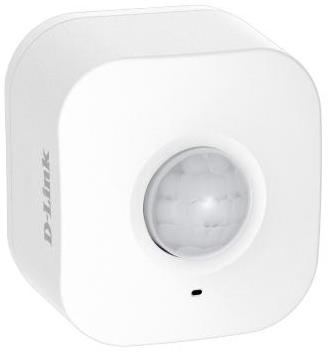
\includegraphics[width=0.4\textwidth]{images/Chapter_04/d-link-motion-sensor.jpg}
	\caption{The D-Link DCH-S150 motion sensor}
	\label{fig:d-link-motion-sensor}
\end{figure}

\subsubsection{D-Link Smart Home Devices}
OpenHAB supports the D-Link DCH-S150 (figure \ref{fig:d-link-motion-sensor}), a WiFi motion sensor.\\~\\
Pros:
\begin{itemize}
	\item Easy to install and very useful for a smart home, no special configuration needed
	\item Communication via API (OpenHAB binding)
\end{itemize}

\subsubsection{EnOcean Sensor Solutions}
EnOcean provides reliable and self-powered wireless sensor solutions for the Internet of Things. This binding allows openHAB
to monitor and control EnOcean devices through the EnOcean USB 300 gateway. EnOncean sensors include rocker switches,
environment sensors and contact sensors.\\~\\
What to consider:
\begin{itemize}
	\item We need a USB300 stick to control EnOcean devices
\end{itemize}
Pros:
\begin{itemize}
	\item Variety of sensors available
	\item Can work together with many other devices
	\item Communication via API (OpenHAB binding)
\end{itemize}
Cons:
\begin{itemize}
	\item We must have extra hardware to make them work with our system (USB 300 gateway)
\end{itemize}

\subsubsection{X10}
X10 is a company that makes gadgets like cameras and sensors for a Smart Home. This binding makes it possible to control X10 
devices via a server running the Mochad X10 daemon. Mochad is a Linux TCP gateway daemon for the X10 CM15A RF (radio frequency)
and PL (power line) controller and the CM19A RF controller. With the current version of the binding items of type Switch, Dimmer, and 
Rollershutter can be controlled. The binding only uses one-way communication so no status reading\\~\\
Pros:
\begin{itemize}
	\item Relatively low price
	\item Communication via API (OpenHAB binding)
\end{itemize}
Cons:
\begin{itemize}
	\item Low availability in Europe, mainly via specialised shops
	\item Needs extra software
	\item Offers less control than other devices
\end{itemize}

\subsection{Smart TV}

\subsubsection{LG TV}
This binding supports LG TV models with Netcast 3.0 and Netcast 4.0 (Model years 2012 and 2013), and with LG TVs which support the
UDAP 2.0 protocol over Ethernet.\\~\\
Pros:
\begin{itemize}
	\item LG Smart TVs are a very common device that should be supported by our system
	\item Communication via API (OpenHAB binding)
\end{itemize}
Cons:
\begin{itemize}
	\item OpenHAB documentation is not very specific about this binding
	\item It does not appear to support more modern LG televisions
\end{itemize}

\subsubsection{Panasonic TV}
This binding supports Panasonic TVs. It should be compatible with most up-to-date Panasonic Smart-TVs.\\~\\
Pros:
\begin{itemize}
	\item It is possible to control the TV completely from the system
	\item Panasonic TVs are a very common device
	\item Easy configuration
	\item Communication via API (OpenHAB binding)
\end{itemize}

\subsubsection{Samsung TV}
This binding integrates the Samsung TV’s.\\~\\
What to consider:
\begin{itemize}
	\item Samsung TV C (2010), D (2011), E (2012) and F (2013) models should be supported. Because Samsung does not publish any
	documentation about the TV’s UPnP interface, there could be differences between different TV models, which could lead to mismatch
	problems.
\end{itemize}
Pros:
\begin{itemize}
	\item Support for Samsung TVs is truly necessary, as they are one of the biggest Smart TV resellers
\end{itemize}
Cons:
\begin{itemize}
	\item Very limited control of the TV
	\item It has not been tested much, so we really do not have many information about this binding and if it will work with other models
\end{itemize}

\subsection{Temperature Control}

\begin{figure}
	\centering
	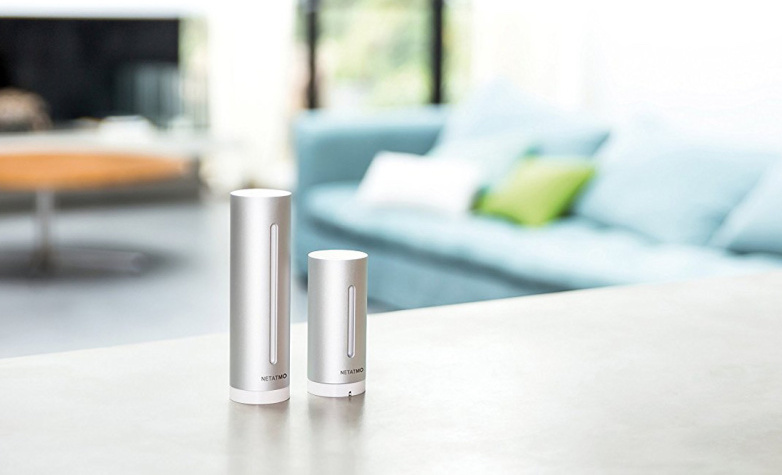
\includegraphics[width=1\textwidth]{images/Chapter_04/netatmo-weather-station.jpg}
	\caption{The Netatmo Personal Weather Station}
	\label{fig:netatmo-weather-station}
\end{figure}

\subsubsection{Devices using eBUS protocol}
The eBUS binding allows controlling the heating system. The eBUS protocol is used by heating system vendors like Wolf, Vaillant,
Kromschröder etc. It is possible to read temperatures, pump performance, gas consumption etc.\\~\\
Pros:
\begin{itemize}
	\item One of the main purposes of this Smart Home Controller is covering heating devices, thanks to this binding it is possible.
	\item Communication via API (OpenHAB binding)
\end{itemize}
Cons:
\begin{itemize}
	\item Quite complex to implement 
\end{itemize}

\subsubsection{EcoTouch Binding}
The openHAB EcoTouch binding allows interaction with Waterkotte EcoTouch heat pumps.\\~\\
Pros:
\begin{itemize}
	\item Communication via API (OpenHAB binding)
\end{itemize}

\subsubsection{MAX! Thermostats}
This is the binding for the eQ-3 MAX! Home Solution. This binding allows you to integrate, view and control the MAX! Thermostats 
in the openHAB environment.\\~\\
What to consider:
\begin{itemize}
	\item Discovery: when the Cube is found, it will become available in the discovery Inbox. Periodically the network is queried again
	for a Cube. Once the Cube is available in openHAB, all the devices connected to it are discovered and added to the discovery inbox.
	No scan is needed to trigger this.
\end{itemize}
Pros:
\begin{itemize}
	\item Communication via API (OpenHAB binding)
	\item Useful and multipurpose. For example, it is possible to track the temperature of the heating devices anytime 
\end{itemize}
Cons:
\begin{itemize}
	\item Extra device needed: MAX! Cube. It is also possible to communicate with these devices using a CUL USB Dongle rather than
	the MAX! Cube.
\end{itemize}

\subsubsection{Netatmo}
The Netatmo binding integrates the following Netatmo products:
\begin{itemize}
	\item Personal Weather Station (figure \ref{fig:netatmo-weather-station}): reports temperature, humidity, air pressure, carbon 
	dioxide concentration in the air, as well as the ambient noise level.
	\item Thermostat: reports ambient temperature, allow to check target temperature, consult and change furnace heating status....
\end{itemize}
What to consider:
\begin{itemize}
	\item Discovery: Netatmo Binding is able to discover automatically all depending modules and devices from Netatmo website. It is 
	also possible to add manually devices by creating things in in the *.things file.
\end{itemize}
Pros:
\begin{itemize}
	\item Good-looking and easy to install solutions for temperature control and temperature information
	\item Communication via API (OpenHAB binding)
\end{itemize}
Cons:
\begin{itemize}
	\item Too expensive for our price range (EUR 179 for the thermostat and EUR 169 for the weather station)
\end{itemize}

\subsection{WiFi Sockets}

\subsubsection{Orvibo S20}
This binding integrates Orvibo devices that communicate using UDP. Only supports Orvibo S20 WiFi sockets.\\~\\
Pros:
\begin{itemize}
	\item Smart Plugs enable controlling and automating non-smart devices from the controller
	\item Orvibo offers unexpensive and easy devices for this matter
	\item Communication via API (OpenHAB binding)
\end{itemize}

\subsection{Xiaomi Mi Smart Home}

This binding allows openHAB to communicate with the Xiaomi Smart Home Suite. This includes the following devices:
\begin{itemize}
	\item Xiaomi Smart Gateway v2 (with radio support)
	\item Xiaomi Smart Temperature and Humidity Sensor (round one)
	\item Xiaomi Smart Door/Window Sensor (round one)
	\item Xiaomi Wireless Switch (round one)
	\item Xiaomi Motion Sensor / IR Human Body sensor
	\item Xiaomi Smart Plug
	\item Xiaomi Smart Magic Cube
	\item Xiaomi Aqara ZigBee Wired Wall Switch (1 and 2 buttons)
	\item Xiaomi Aqara ZigBee Wireless Wall Switch (1 and 2 buttons)
	\item Xiaomi Aqara Smart Curtain
	\item Xiaomi Aqara Water Leak Sensor
	\item Xiaomi Aqara Wireless Switch (square one)
	\item Xiaomi Aqara Temperature, Humidity and Pressure Sensor (square one)
	\item Xiaomi Aqara Door/Window Sensor (square one)
	\item Xiaomi Aqara Motion Sensor (with light intensity support)
	\item Xiaomi Mijia Honeywell Gas Alarm Detector
	\item Xiaomi Mijia Honeywell Fire Alarm Detector
\end{itemize}
What to consider:
\begin{itemize}
	\item The MiHome app is necessary in order to connect the Gateway
\end{itemize}
Pros:
\begin{itemize}
	\item Xiaomi is an extremely affordable brand that offers many devices for Home Automation. 
	\item Easy to install and configure
	\item Communication via API (OpenHAB binding)
\end{itemize}
Cons:
\begin{itemize}
	\item Needs extra hardware (Smart Gateway) and software (MiHome app)
\end{itemize}

\subsection{Other devices and services}

\subsubsection{Logitech Harmony  Hub}
The Harmony Hub binding is used to enable communication between openHAB2 and multiple Logitech Harmony Hub devices. Logitech Smart
Hub devices can control other devices like Apple TV, Amazon Alexa, or Sonos devices. The Binding works as a bridge between the Harmony 
Hub and the devices connected to it.\\~\\
Pros:
\begin{itemize}
	\item Might be beneficial to consider it given the fact that there could be devices (with proprietary communication protocols) that 
	we wouldn’t be able to support, like Apple TV
	\item Communication via API (OpenHAB binding)
\end{itemize}
Cons:
\begin{itemize}
	\item Limited API
\end{itemize}

\subsubsection{Epson Projectors}
This binding is compatible with Epson projectors which support ESC/VP21 protocol over serial port.\\~\\
Pros:
\begin{itemize}
	\item Communication via API (OpenHAB binding)
\end{itemize}
Cons:
\begin{itemize}
	\item Seems that only business-oriented projectors are compatible with this binding
\end{itemize}

\subsubsection{MQTT}
This binding allows openHAB to act as an MQTT (MQ Telemetry Transport) client, so that openHAB items can send and receive MQTT 
messages from or to an MQTT broker.\\~\\
What to consider:
\begin{itemize}
	\item Implementing MQTT makes us able to use OwnTracks, a location service that uses MQTT that focuses on privacy.
\end{itemize}

\subsubsection{NTP}
The NTP binding is used for displaying the local date and time based update from an NTP server. Discovery is used to place one default 
tem in the inbox as a convenient way to add a Thing for the local time.

\subsubsection{Weather Binding}
The Weather binding collects current and forecast weather data from different providers with a free weather API. You can also display
weather data with highly customizable HTML layouts and icons. It is also possible to install the WeatherUnderground and YahooWeather
bindings.

\bigskip
\section{Voice Assistants}
The objective of this section is to explore the main voice assistants available commercially. As I explained previously, the services
provided by virtual assistants, and in particular voice assistants, are very varied. One of them is smart home control, and many of
the home-oriented voice assistants provide it. The focus on this section will be on them, the most closely related to my project.

\subsection{Samsung Bixby}
Bixby is the virtual assistant that Samsung includes in their phones, introduced in 2017, along with the introduction of the Samsung
Galaxy S8 phone. It is the evolution of their previous voice assistant, \textit{S Voice}.

Bixby is divided in three parts: \textit{Bixby Voice}, which is the voice assistant, \textit{Bixby Vision}, an assistant that works through
image recognition, and \textit{Bixby Home}, a dashboard that provides different information depending on the current
conditions.\cite{samsungBixby}

Bixby has been widely criticized for his intrusiveness and its lack of utility in many situations. In addition, it is only available in English
and Chinese at this moment. As for home automation, it is seamlessly integrated with Samsung SmartThings, making it possible to send
basic commands to devices via voice.

\subsection{Google Assistant}
Google Assistant is the name of the virtual assistant developed by Google. It was introduced in 2016, and at this moment it is
available for mobile phones (with Android and iOS operating systems), laptops, TVs, cars and smart watches. It is also integrated in
Google Home, their smart speaker.\cite{googleAssistant}

The most remarkable feature of this assistant is its ability to engage in two-way conversations, thanks to a powerful artificial intelligence
developed by Google, and Google Duplex, a new technology that Google is developing, which will allow it to have natural conversations,
mimicking the human voice.

Google Assistant is able to manage a wides range of smart home devices and in a very flexible way, thanks to its outstanding voice
recognition.

\subsection{Apple Siri}
Siri is the voice assistant developed by Apple, and the one who began the revolution of voice assistance in mobile phones. Introduced
back in 2011 and included in the iPhone 4S, it has been present in all the iOS devices (iPhones, iPads and iPods) since then, and lately
in the macOS devices (Macintosh computers) and in the Apple Watch as well.\cite{appleIOSSiri} Its range of functionalities is also
similar to its competitors, but with a slightly narrower range of possible interactions, which can make Siri feel a little less natural.

In later iOS versions, Apple has implemented Siri suggestions, which use the artificial intelligence that Siri provides to suggest
applications to the user based in the current circumstances. Siri is able to adapt over time to the user's personal preferences by
customizing search results and other responses. In the latest version of iOS, iOS 11, Siri has a much more natural voice, that can
also simulate different moods.

\subsection{Amazon Alexa}
Alexa is the virtual assistant by Amazon, and it is included by default in all their Echo devices (Amazon's smart speakers), Fire TVs
(digital media players) and Fire tablets. It is also available for iOS and Android devices as a standalone application. Its capabilities are
very similar to those of its competitors: music playback, making to-do lists, setting alarms, playing podcasts and audiobooks, providing
information, such as weather forecast and general knowledge, and of course voice interaction and home automation management.
This means that, as in the previous cases, there is also a home automation system underlying the assistant in Alexa.

Alexa differentiates from the rest on its skill system. A \textit{skill} is a functionality developed by a third-party vendor that the user
can install in the assistant in order to extend is capabilities. They can be, for instance, news services or little games. Amazon is
constantly encouraging the creation of new skills for Alexa between the developer community.\cite{amazonAlexa}

\subsection{Mycroft}
Mycroft is the name of a suite of software and hardware tools that use natural language processing and machine learning to provide
an open source voice assistant.\cite{mycroftDocumentation} Unlike the other virtual assistant we have seen previously, Mycroft is
fully open source and free. It has been undergoing heavy development since late 2017, but now it claims to be usable effectively
by developers and enthusiasts, making it the world's first fully open source AI voice assistant. But unfortunately, it is not yet usable
by the general user, as it still requires technical skills.

Mycroft is available for Linux-based operating systems and Android, but it is not ready yet for macOS and Windows, making it harder
to spread as quickly as other virtual assistants have done. However, to make up for this, they are selling their own smart speaker,
called Mark, currently in its second version.

Mycroft is modular, which makes the system easily customizable, and uses a skill system similar to Amazon Alexa. It comes with a
number of default skills, such as setting an alarm, providing the weather, or telling the time. The other skills are also installable via
voice commands, based on a list of community-contributed skills. The number of additional skills is not as high as in Alexa, but it
is constantly growing, and Mycroft encourages its users to contribute to the project.

\bigskip
The table \ref{table:voice-assistants-comparison} shows a comparison between the most important aspects of the previous voice
assistants. In this table, note that \textit{Smart Home} means having Home Automation capabilities, and always on means that the
user is able to trigger the assistant via the voice. For example, Siri is able to react to the sentence \textit{Hey Siri!}, even if the
device is with the screen off.

\begin{table}[]
	\begin{center}
		\resizebox{\textwidth}{!}{
		\begin{tabular}{|l|l|p{0.08\linewidth}|p{0.09\linewidth}|p{0.18\linewidth}|l|l|p{0.1\linewidth}|}
			\hline
			\textbf{Name} & \textbf{Developer}                                                          & \textbf{Free} & \textbf{Open source} & \textbf{Home Automation}                                    & \textbf{Mobile app}                                            & \textbf{Extra devices}                                                              & \textbf{Always on} \\ \hline
			Bixby         & Samsung                                                                     & No            & No                   & \begin{tabular}[l]{@{}l@{}}Yes\\- SmartThings\end{tabular} & \begin{tabular}[l]{@{}l@{}}Yes\\ Samsung phones\end{tabular} & No                                                                                  & Yes                \\ \hline
			Assistant     & Google                                                                      & No            & No                   & Yes                                                         & \begin{tabular}[l]{@{}l@{}}Yes\\ Android\end{tabular}        & Google Home                                                                         & Yes                \\ \hline
			Siri          & Apple                                                                       & No            & No                   & \begin{tabular}[l]{@{}l@{}}Yes\\- HomeKit\end{tabular}     & \begin{tabular}[l]{@{}l@{}}Yes\\ iOS\end{tabular}            & HomePod                                                                             & Yes                \\ \hline
			Alexa         & Amazon                                                                      & No            & No                   & Yes                                                         & \begin{tabular}[l]{@{}l@{}}Yes\\ iOS, Android\end{tabular}   & \begin{tabular}[l]{@{}l@{}}Echo\\ Echo Dot\\ Echo Dot Kids\\ Echo Plus\end{tabular} & Yes                \\ \hline
			Mycroft       & \begin{tabular}[l]{@{}l@{}}Mycroft and the\\ Mycroft Community\end{tabular} & Yes           & Yes                  & Yes                                                         & \begin{tabular}[l]{@{}l@{}}Yes\\ Android\end{tabular}        & \begin{tabular}[l]{@{}l@{}}Mark II\\ Mark I\end{tabular}                            & Yes                \\ \hline
		\end{tabular}}
	\caption{Comparison between different voice assistants}
	\label{table:voice-assistants-comparison}
	\end{center}
\end{table}


\chapter{OpenHAB}

After analyzing the main products and services in the field of home automation and voice assistance, we must choose the solution
that can best fit this project. One of its requirements is to use as many open source and free technologies as possible, and that
the final product is easily usable by the final user and sufficiently flexible to adapt it to our needs.

OpenHAB is fully open source and completely free, and has reached a level of maturity where it is highly stable and intuitive. In its
most recent version, it provides an user interface that automatize many tasks that a standard user might not know how to do. And,
of course, it can integrate many devices from different vendors, as In have mentioned in the previous chapters, which is also one of
the most important matters for reaching our objective.

In this chapter, we will explore in depth this home automation platform and all its possibilities, in order to have a better general idea
about it when building the final system.

\section{Introduction}
As mentioned in previous chapters, openHAB (open Home Automation Bus) is a completely free, technology agnostic and open
source platform for home automation.

OpenHAB software is capable of integrating different domotic systems, devices and technologies into a single solution. It also
provides uniform user interfaces, and a common approach to automation rules across the entire system, regardless of the number
of manufacturers and sub-systems involved.\cite{openHABDocs}

The platform runs on many popular platforms including Linux, Windows and macOS. It is also popular to install it in systems like the
Raspberry Pi, and openHAB even provides a special distribution for this computer, called \textit{openHABian}, a simplified way of
getting up and running openHAB, but offering the complete experience.

OpenHAB defines also a community of users, contributors and maintainers, working together on the improvement of the system.
Everything related to the community is in the openHAB community forum. The community is very active and helpful, and thanks
to them we have always found a way to solve our issues.

\bigskip
\section{History of openHAB}
The history of openHAB begins in 2010, when Kai Kreuzer, a smart home enthusiast from Germany, developed in Java and using the
OSGi technology (Open Services Gateway Initiative) as the basis, which is a set of specifications that define a dynamic component
system for Java. The use of this technology makes it easier to update the services independently and their implementation. It favor
the expandability of the system.

In 2013, openHAB becomes an official Eclipse project under the name of Eclipse SmartHome, but they decide to keep both projects
active and to develop them at the same time. In Eclipse SmartHome would maintain the architecture and the functionalities from the
previous openHAB, and in openHAB they would study how to integrate the different devices and technologies that it supports via
add-ons.

The newest version, OpenHAB 2, has been the biggest change that OpenHAB has suffered since its initial launch. It includes more
add-ons and some changes that simplify much more the process for developers, as well as implementing Apache Karaf underneath,
which greatly extends its possibilities. In addition, the UIs have been improved, improving greatly the user experience. OpenHAB 2 is
much easier to install, and it automates many repetitive processes that might result hard for some users.

\bigskip
\section{Structure}
OpenHAB works thanks to add-ons, which can extend its capabilities to fit each user’s needs, from User Interfaces, to the ability to
interact with a large and growing number of physical \textit{Things}. Add-ons may come from the OpenHAB 2 distribution, the Eclipse
SmartHome project Extensions, or from the OpenHAB 1 distribution.

\begin{figure}
	\centering
	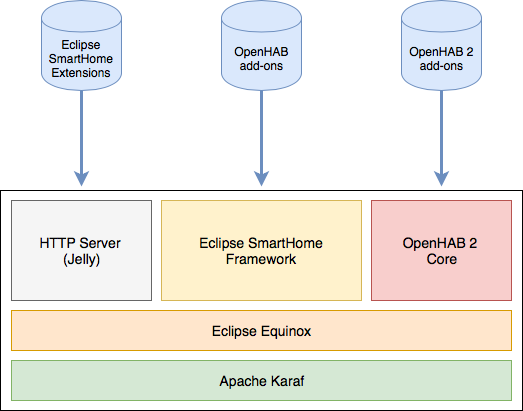
\includegraphics[width=0.9\textwidth]{images/Chapter_05/openhab-architecture.png}
	\caption{OpenHAB architecture}
	\label{fig:openhab-architecture}
\end{figure}

The figure \ref{fig:openhab-architecture} shows the overall architecture of openHAB 2. In the lowest layer, we can find Apache Karaf.
Apache Karaf is basically a modular and open source OSGi runtime environment that can host any kind of applications.\cite{apacheKaraf}

Next, there is Eclipse Equinox, which is also an implementation of the OSGi core framework specification. But the goal of the Equinox
project is to be a first class OSGi community and foster the vision of Eclipse as a landscape of bundles too. Equinox is responsible for
developing and delivering the OSGi framework implementation used for all of Eclipse.\cite{eclipseEquinox}

The next and last level is divided in three parts. The first one is the Jetty HTTP server, also part of Eclipse, which provides a Web server
and javax.servlet container, plus support for HTTP/2, WebSocket, OSGi, JMX, JNDI and JAAS, among others.\cite{eclipseJetty} Secondly,
we can find the Eclipse SmartHome Framework , the framework to build end user solutions on top like openHAB, that we mentioned
before.\cite{eclipseSmartHomeDocs} The last part is the core of openHAB 2, which provides the full solution.

As the diagram in the figure \ref{fig:openhab-architecture} indicates, we can add to this system extensions from Eclipse SmartHome and
add-ons from the first and second version of openHAB.

\bigskip
\section{Concepts}
As Eclipse SmartHome is the logic part of OpenHAB 2, all the elements we are listing are part of it. Eclipse SmartHome strictly differentiates
between the physical view and the functional view of the system. The physical view is more familiar to us, and focuses on the devices
on the system, the connections between them (e.g. wires, Netatmo devices, WiFi hardware) and other physical aspects of the system.
The functional view focuses on how information about the devices, connections, and so on, is represented in user interfaces, focusing
on how rules effect representations of physical devices in software. The functional view focuses on how an action in a user interface
affects the software associated with the physical device it represents.\cite{openHABDocs}

That said, the different elements that Eclipse SmartHome differentiates will be explored in this section. The greatest difference
that we can findrelated to devices, is between \textit{Things} and \textit{Items}. Generally speaking, Things represent physical
systems that can be added to openHAB and Items represent functionalities that can be used by the applications. The figure
\ref{fig:openhab-concepts-basics} shows a graphical explanation of this concept, though we will explain these concepts in depth below.

\begin{figure}
	\centering
	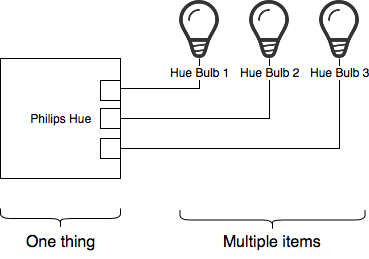
\includegraphics[width=0.6\textwidth]{images/Chapter_05/openhab-concepts-basics.png}
	\caption{A simplification of the concepts of Thing and Item}
	\label{fig:openhab-concepts-basics}
\end{figure}

\subsection{Things}
Things are the entities that can physically be added to a system and which can potentially provide many functionalities in one. They do
not need to be devices, but they can also represent a web service, or any other manageable source of information and functionality.
Things are important in the setup and configuration process, when the user has to add his devices to the system, but they are not for
the operation, when everything is up and running.

Things can have configuration properties, which can be optional or mandatory. Such properties can be basic information like an IP address,
an access token for a web service or a device specific configuration that alters its behavior.

\subsubsection{Channels}
Channels are part of the Things, and they represent the different functions they provide. Where the Thing is the physical entity
or source of information, the Channel is a concrete function from this Thing. For example, some Philips Hue light bulbs have a color
temperature Channel and a color Channel, both providing functionality of the one light bulb Thing to the system. For sources of
information the Thing might be the local weather with information from a web service with different Channels like temperature, pressure
and humidity.

Channels are linked to Items, where such links are the glue between the virtual and the physical layer. Once such a link is established,
a Thing reacts on events sent for an item that is linked to one of its Channels. Likewise, it actively sends out events for Items linked to its
Channels

\subsubsection{Bridges}
Bridges are special types of Things. They are \textit{Things} that need to be added to the system in order to gain access to other Things.
For example, an IP gateway for some non-IP based home automation system or a web service configuration with authentication information
which every Thing from this web service might need.

Some Bindings come with a Bridge, like the \textit{PHC Binding}, which allows to integrate modules of PHC in openHAB.\cite{openHABPHCBinding}

\subsubsection{Thing Status}
Every Thing has a status, which helps to identify possible problems with the device or service and gives useful information to the user
in any moment. The statuses are limited to seven types, as the table \ref{table:thing-statuses} shows.

\begin{table}[]
	\begin{center}
		\resizebox{\textwidth}{!}{
		\begin{tabular}{|c|p{0.8\linewidth}|}
			\hline
			\textbf{Status} & \multicolumn{1}{c|}{\textbf{Description}}                                                                                                                                                                                                                                                                                                                                                                                                                                                 \\ \hline
			UNINITIALIZED & This is the initial status of a Thing, when it is added or the framework is being started. This status is also assigned, if
			the initializing process failed or the binding is not available. Commands, which are sent to Channels will not be processed. \\ \hline
			INITIALIZING & This state is assigned while the binding initializes the Thing. It depends on the binding how long the initializing process
			takes. Commands, which are sent to Channels will not be processed. \\ \hline
			UNKNOWN & The handler is fully initialized but due to the nature of the represented device/service it cannot really tell yet whether the
			Thing is ONLINE or OFFLINE. Therefore the Thing potentially might be working correctly already and may or may not process commands.
			But the framework is allowed to send commands, because some radio-based devices may go ONLINE if a command is sent to them. The
			handler should take care to switch the Thing to ONLINE or OFFLINE as soon as possible. \\ \hline
			ONLINE & The device/service represented by a Thing is assumed to be working correctly and can process commands. \\ \hline
			OFFLINE & The device/service represented by a Thing is assumed to be not working correctly and may not process commands. But the
			framework is allowed to send commands, because some radio-based devices may go back to ONLINE, if a command is sent to them. \\ \hline
			REMOVING & The device/service represented by a Thing should be removed, but the binding did not confirm the deletion yet. Some
			bindings need to communicate with the device to unpair it from the system. Thing is probably not working and commands can not be
			processed. \\ \hline
			REMOVED & This status indicates that the device/service represented by a Thing was removed from the external system after the
			REMOVING was initiated by the framework. Usually this status is an intermediate status because the Thing gets removed from the
			database after this status was assigned. \\ \hline
		\end{tabular}}
	\caption{Statuses of Things in openHAB 2}
	\label{table:thing-statuses}
	\end{center}
\end{table}

The statuses UNINITIALIZED, INITIALIZING and REMOVING are set by the framework, where as the statuses UNKNOWN, ONLINE and OFFLINE
are assigned from a binding. Additionally, the REMOVED state is set by the binding to indicate that the removal process has been completed,
that it, the Thing must have been in REMOVING state before.

\subsubsection{Status Transitions}
The figure \ref{fig:status-transitions} shows the possible status transitions in openHAB.

\begin{figure}
	\centering
	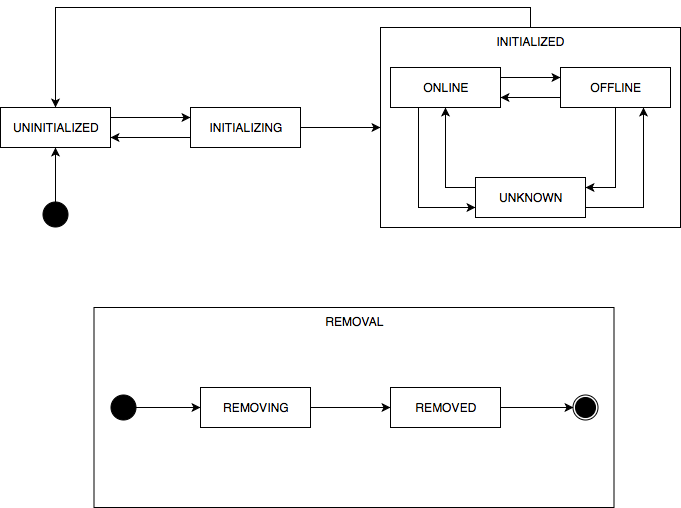
\includegraphics[width=1\textwidth]{images/Chapter_05/status-transtitions.png}
	\caption{Thing status transitions}
	\label{fig:status-transitions}
\end{figure}

The initial state of a Thing is UNINITIALIZED. From UNINITIALIZED the Thing goes into INITIALIZING. If the initialization fails, the
Thing goes back to UNINITIALIZED. If the initialization succeeds, the binding sets the status of the Thing to UNKNOWN, ONLINE
or OFFLINE, which all mean that the Thing handler is fully initialized. From one of this states the Thing can go back into UNINITIALIZED,
REMOVING or REMOVED. The statuses REMOVING and REMOVED can also be reached from any of the other states.

\subsection{Items}
Eclipse SmartHome has a strict separation between the physical world (Things) and the application, which is built around the concept
of \textit{Items} (also known as the \textit{virtual layer}).

As mentioned at the beginning of this section, Items represent functionalities that can be used by the applications, mainly user
interfaces or automation logic. Items also have a state and are used through events.

Each openHAB Item must be between the list of types that the table \ref{table:openhab-item-types} specifies.

\begin{table}[]
	\centering
	\resizebox{\textwidth}{!}{%
		\begin{tabular}{|l|l|l|}
			\hline
			\multicolumn{1}{|c|}{\textbf{Type}}                          & \multicolumn{1}{c|}{\textbf{Description}}                                                                          & \multicolumn{1}{c|}{\textbf{Command Types}}                                           \\ \hline
			Color                                                         & Color information (RGB)                                                                                            & \begin{tabular}[c]{@{}l@{}}OnOff, IncreaseDecrease,\\ Percent, HSB\end{tabular}       \\ \hline
			Contact                                                       & \begin{tabular}[c]{@{}l@{}}Item storing status of e.g. door/window \\ contacts\end{tabular}                        & OpenClose                                                                             \\ \hline
			DateTime                                                      & Stores date and time                                                                                               &                                                                                       \\ \hline
			Dimmer                                                        & \begin{tabular}[c]{@{}l@{}}Item carrying a percentage value for \\ dimmers\end{tabular}                            & \begin{tabular}[c]{@{}l@{}}OnOff, IncreaseDecrease,\\ Percent\end{tabular}            \\ \hline
			Group                                                         & \begin{tabular}[c]{@{}l@{}}Item to nest other Items / collect them \\ in Groups\end{tabular}                       &                                                                                       \\ \hline
			Image                                                         & Holds the binary data of an image                                                                                  &                                                                                       \\ \hline
			Location                                                      & Stores GPS coordinates                                                                                             & Point                                                                                 \\ \hline
			Number                                                        & \begin{tabular}[c]{@{}l@{}}Stores values in number format, takes \\ an optional dimension suffix\end{tabular}      & Decimal                                                                               \\ \hline
			\begin{tabular}[c]{@{}l@{}}Number\\ $<$dimension$>$\end{tabular} & \begin{tabular}[c]{@{}l@{}}Like Number, but with additional \\ dimension information for unit support\end{tabular} & Quantity                                                                              \\ \hline
			Player                                                        & \begin{tabular}[c]{@{}l@{}}Allows to control players (e.g. \\ audio players)\end{tabular}                          & \begin{tabular}[c]{@{}l@{}}PlayPause, NextPrevious, \\ RewindFastforward\end{tabular} \\ \hline
			Rollershutter                                                 & Typically used for blinds                                                                                          & \begin{tabular}[c]{@{}l@{}}UpDown, StopMove, \\ Percent\end{tabular}                  \\ \hline
			String                                                        & Stores texts                                                                                                       & String                                                                                \\ \hline
			Switch                                                        & Typically used for lights                                                                                          & OnOff                                                                                 \\ \hline
		\end{tabular}%
	}
	\caption{Types of Items in openHAB 2}
	\label{table:openhab-item-types}
\end{table}

\subsubsection{Group Items}
Group Items are a special kind of items that collect other Items into Groups. Group Items can themselves be members of other Group Items.
Depending on the user interface, it might display Group Items as single entries and provide navigation to its members.

With Group Items, it is also possible to derive their state from their member items. To derive a state the Group Item must be constructed using
a base Item and a Group function. Between the available Group functions we can find common operators such as EQUALITY, AND, OR, NAND,
NOR, SUM, AVG, MIN and MAX, among others.

\subsubsection{Links}
Links are the glue between Things and Items. They are associations between exactly one Thing Channel and one Item. If a Channel is
linked to an Item, it is enabled, which means that the functionality that the Item represents is handled through the given Channel.
Channels can be linked to multiple Items and Items can be linked to multiple Channels.

\subsection{Thing Discovery}
Thing Discovery is the process that the system makes in order to show the devices connected in your network. Many technologies,
devices and systems can be discovered automatically or browsed through an API.

In Eclipse SmartHome bindings implement \textit{Discovery Services} for Things, which provide \textit{Discovery Results}. All Discovery
Results are regarded as suggestions to the user and are put into the \textit{Inbox}.

\subsubsection{Inbox}
The Inbox holds a list of all discovered Things from all active discovery services. A discovery result represents a discovered Thing of a
specific Thing type, that could be instantiated as a Thing. The result usually contains properties that identify the discovered Things
further like IP address or a serial number. Each discovery result also has a timestamp when it was added to or updated in the Inbox
and it may also contain a time to live, indicating the time after which it is be automatically removed from the Inbox.

Discovery results can either be ignored or approved, where in the latter case a Thing is created for them and they become available in
the application. If an entry is ignored, it will be hidden in the Inbox without creating a Thing for it.

Eclipse SmartHome offers a service that is capable of automatically ignore discovery results on the Inbox, whenever a Thing is created
manually, that represents the same Thing, as the respective discovery result would create. This Thing would either have the same Thing
UID or the value of its representation property is equal to the representation property's value in the discovery result. The service is
enabled by default.

\subsection{Audio and Video}
Audio and voice features are an important aspect of any smart home solution as it is a very natural way to interact with the user.

Eclipse SmartHome comes with a very modular architecture that makes it possible in plenty of situations. At its core, there is the notion
of an \textit{audio stream}. Audio streams are provided by \textit{audio sources} and consumed by \textit{audio sinks}.

\begin{itemize}
	\item \textbf{Audio Streams} are essentially a byte stream with a given audio format.
	\item \textbf{Audio Formats} define the container (e.g. WAV), encoding, bit rate, sample frequency and depth and the bit order (little endian
	or big endian).
	\item \textbf{Audio Sources} are services capable of producing audio streams, which are able to support different formats and provide a
	stream in a requested format upon request. Typical audio sources are microphones, and a continuous stream is expected from them.
	\item \textbf{Audio Sinks} are services that accept audio streams of certain formats. Typically, these are expected to play the audio stream,
	for example, a speaker.
	\item \textbf{Text-to-Speech (TTS)} services are similar to audio sources with respect to the ability to create audio streams. The different
	is that they take a string as an input and will synthesize it to a spoken text using a given voice.
	\item \textbf{Speech-to-Text (STT)} services are similar to audio sinks, but they do not simply play back the stream, but convert it to a
	plain string.
\end{itemize}

\begin{figure}
	\centering
	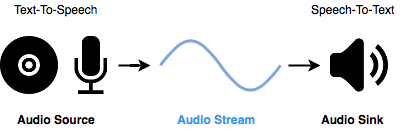
\includegraphics[width=0.7\textwidth]{images/Chapter_05/oh-audio-stream.png}
	\caption{Eclipse SmartHome audio stream scheme}
	\label{fig:oh-audio-stream}
\end{figure}

TTS and STT can provide information about the voices that they support, formats and locales. In TTS, each voice supports exactly one
locale.

However, the STT service itself does not seem to be very useful. In order to process the generated string, there is the concept of a
\textit{human language interpreter}.

\subsubsection{Human Language Interpreter}
A Human Language Interpreter takes a string as an input. It then derives actions from it, like sending commands to devices, or replies
with a string, which opens the possibility to realize conversations. The figure \ref{fig:human-language-interpreter} shows a simple
schema of how it works.

In fact, an interpreter is not directly related to audio streams, but operates only with strings, so it is suitable either for voice
assistants or chatbots for console, Twitter or other messaging services.

\begin{figure}
	\centering
	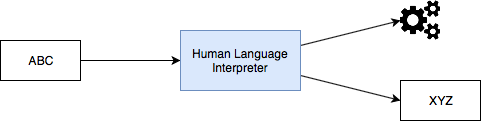
\includegraphics[width=0.9\textwidth]{images/Chapter_05/human-language-interpreter.png}
	\caption{A Human Language Interpreter transforms strings into other strings or commands}
	\label{fig:human-language-interpreter}
\end{figure}

Applications can dynamically choose which services to use, so that different sinks can be used for different use cases. Defaults can be
set as configuration for all those services in case an application does not ask for any specific service.

\bigskip
\section{A Developer Perspective on openHAB}
OpenHAB 2 is a great open source, technology agnostic home automation platform that is able to manage lots of smart services and devices.

However, from a developer point of view, OpenHAB is not a complete platform itself, but rather an aggregation of features from different
repositories, and mainly from Eclipse SmartHome:

\begin{itemize}
	\item \textbf{Eclipse SmartHome Framework}: the major parts of the core functionality are held by this repository. It contains bindings,
	services and items, amongst others, as openHAB does.
	\item \textbf{OpenHAB 2 Core and openHAB add-ons}: add-ons of openHAB that use the Eclipse SmartHome API.
	\item \textbf{Eclipse SmartHome Extensions}: openHAB is compatible with all extensions that are available for the Eclipse SmartHome
	Framework and maintained within their repositories.
\end{itemize}

\subsection{Development environment set up}
Installing the development environment is a different process than installing OpenHAB itself, as a developer would require a local copy of
the source code of all elements, including the bindings, in an IDE.

The process for installing OpenHAB 2 as a developer requires first to install Eclipse IDE with the OpenHAB-related repositories, which are
the ones listed previously. It is usually required to have Maven 3 installed, and it is mandatory to have Oracle JDK 8 beforehand, because
OpenHAB is fully coded in Java. \cite{openHABGithub}

The Eclipse installer downloads a copy of the repositories that the developer selects and installs and integrates them with Eclipse IDE
automatically. Then, user can compile, run and debug the project from the IDE.

\begin{figure}
	\centering
	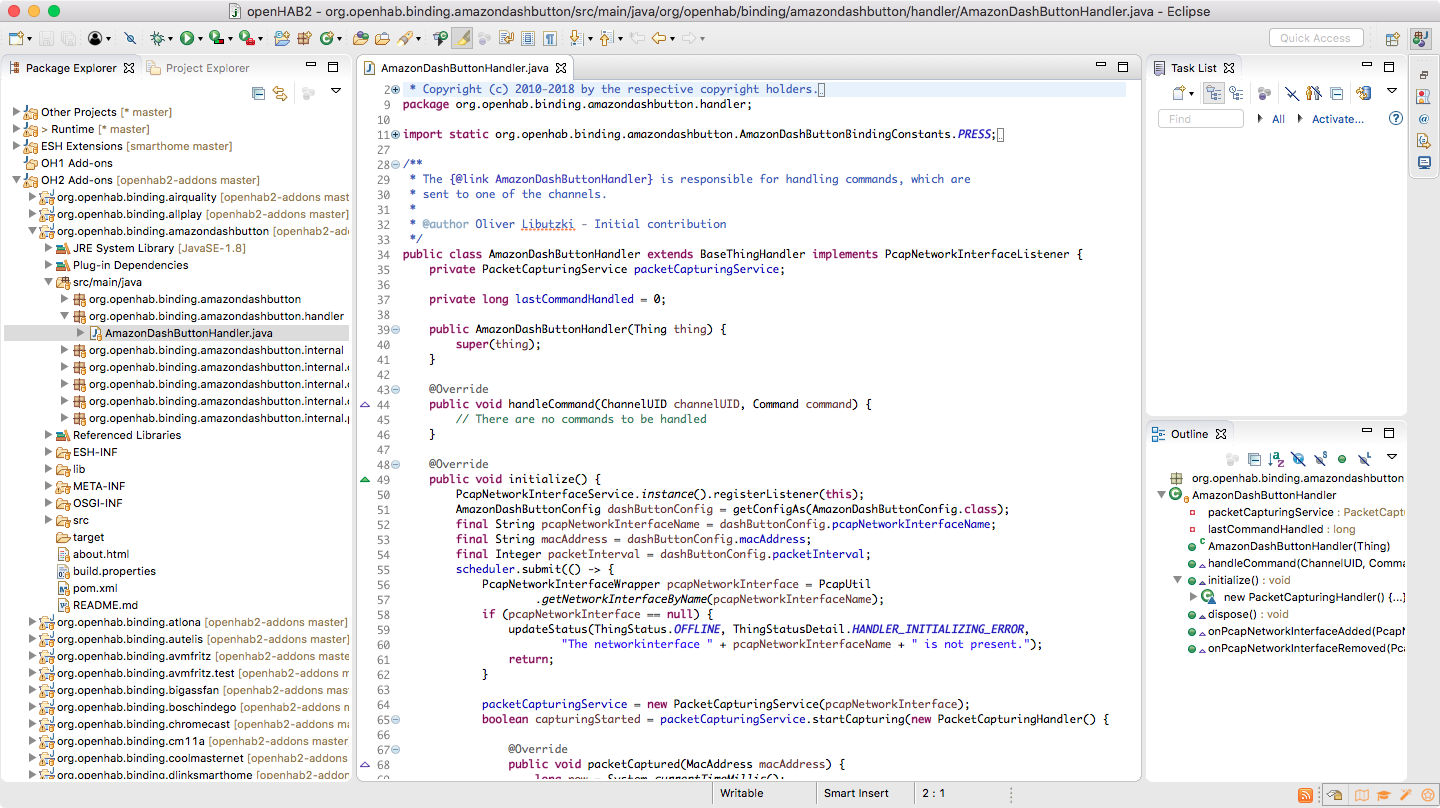
\includegraphics[width=1\textwidth]{images/Chapter_05/openhab2-ide.png}
	\caption{Eclipse SmartHome IDE with the OpenHAB repositories}
	\label{fig:openhab2-ide}
\end{figure}

\subsection{Platform structure}
Installing the platform as mentioned above provides us with a clear knowledge of the platform’s structure and makes it easy to perform
any modification or addition to it. The OpenHAB 2 code is highly modular and presents a very well-defined organization, as can be seen
in the figure \ref{fig:openhab2-structure}. Below there is a detailed explanation about the structure.

\begin{sidewaysfigure}
	\centering
	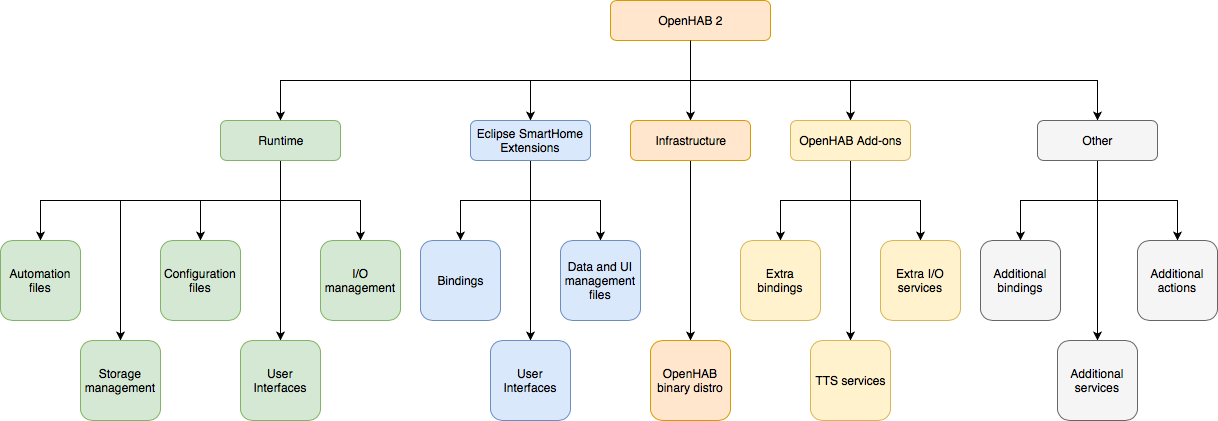
\includegraphics[width=1\textwidth]{images/Chapter_05/openhab2-structure.png}
	\caption{OpenHAB 2 structure}
	\label{fig:openhab2-structure}
\end{sidewaysfigure}

We can divide OpenHAB 2 in five parts, which are composed by one or more subsections that host differentiated code parts, each one
performing services, connecting to devices or managing the internal system:

\begin{itemize}
	\item \textbf{Runtime}: these are the basic libraries that OpenHAB need in order to execute properly, which come mostly from Eclipse
	SmartHome. It is a big collection of different services:
	\begin{itemize}
		\item \textbf{Automation files}: they are in charge of the automated services in the platform, so they manage triggers and events.
		\item \textbf{Configuration files}: hosts the configuration files of the platform, such as the user folders or the listeners for the
		item discovery process.
		\item \textbf{I/O management}: these libraries manage the inputs and outputs of the system, such as the MQTT communication
		or the REST APIs.
		\item \textbf{Storage management}: a pair of libraries that are in charge of storing JSON files and managing MapDB databases.
		\item \textbf{User interfaces}: the user interfaces OpenHAB provides by default are the BasicUI, the ClassicUI, the HomeBuilder
		and the PaperUI (being this the most common in OpenHAB 2, as it requires zero manual configuration). These UIs are all part
		of this repository and they come from OpenHAB, not from Eclipse SmartHome. However, Eclipse also provides packages for
		internal aspects of the UI and for icons.
	\end{itemize}
	\item \textbf{Eclipse SmartHome Extensions}: functionality of Eclipse SmartHome can be extended through different additions, such
	as bindings or other UIs. In this case, we can find:
	\begin{itemize}
		\item \textbf{Bindings}: they are the most important part of our system. Bindings integrate external systems, like services, protocols
		or single devices to the platform. Therefore, the main purpose of a binding is to translate events from the Eclipse SmartHome
		event bus to the external system and vice versa. This repository contains bindings for communicating via Bluetooth, or to Philips
		Hue or DMX devices, amongst others. Many other bindings that OpenHAB support are located in the OpenHAB Add-ons repository.
		\item \textbf{User interfaces}: includes a bunch of UIs from Eclipse SmartHome, from which the OpenHAB UIs were created.
		\item \textbf{Data and UI management files}: this category contains additional configuration files and for managing UI’s elements.
	\end{itemize}
	\item \textbf{Infrastructure}: includes the binary files of OpenHAB. The end-user version of OpenHAB consists in only this repository.
	\item \textbf{OpenHAB add-ons}: these are libraries that OpenHAB introduced to Eclipse SmartHome. They extend its functionality to
	make it a fully usable Home Automation environment.
	\begin{itemize}
		\item \textbf{Extra bindings}: OpenHAB created a huge number of new bindings for Eclipse SmartHome, from the binding for
		Amazon Dash Button to the one for Samsung TVs. They cover an enormous range of smart devices, and the list is constantly growing.
		\item \textbf{Extra I/O services}: some bindings, like the Apple HomeKit binding, require I/O services that Eclipse SmartHome
		does not originally include. In addition, new services like the OpenHAB cloud are also contained here.
		\item \textbf{TTS services}: OpenHAB 2 has added Text-To-Speech and Speech-To-Text functionality to Eclipse SmartHome, which is
		also part of the OpenHAB add-ons repository.
	\end{itemize}
	\item \textbf{Other projects}: this repository holds libraries that are not part of any of the others, and it is a mix of additional bindings
	(EnOcean, FritzBox…), additional actions and more services. Although they are located in this repository, they are officially supported
	by OpenHAB.
\end{itemize}

\subsection{OSGi}
OpenHab is based on OSGi. The OSGi technology is a set of specifications that define a dynamic component system for Java. These
specifications enable a development model where applications are dynamically composed of many different and reusable components.

The OSGi specifications enable components to hide their implementations from other components while communicating through services,
which are objects that are specifically shared between components.\cite{openHABDocs} The main features of OSGi are modularity,
runtime dynamics and service orientation.

\subsubsection{OSGi Containers}
Different containers might implement different parts of the OSGi specifications and might provide slightly different API. The OpenHAB
project uses Equinox, which is the reference implementation of the OSGi R4.x Core Specification and one of the mostly used as well.

Other popular open source OSGi containers are Apache Felix and Concierge. The container ProSyst OSGi Framework is widely used as
well, but it is not free.

\subsubsection{Definitions}
\begin{itemize}
	\item \textbf{Bundle}: the OSGi components made by the developers. A bundle is comprised of Java classes and other resources,
	which together can provide functions to end users.
	\item \textbf{Service}: any object that is registered in the OSGi Service Registry and can be looked up using its interface name(s).
	\item \textbf{Manifest}: descriptive information about the bundle, contained in its JAR file.
	\item \textbf{Service} Registry: enables a bundle to publish objects to a shared registry, advertised via a given set of Java interfaces.
\end{itemize}

\subsubsection{Layer Structure}
As the figure \ref{fig:osgi-layering} shows, the OSGi framework consists of layers build on top of each other:

\begin{itemize}
	\item \textbf{Module layer}: responsible for managing dependencies between bundles and for class loading.
	\item \textbf{Life Cycle Layer}: controls the life cycle of the bundles.
	\item \textbf{Service Layer}: defines a dynamic model of communication between different modules.
	\item \textbf{Actual Services}: this is the application layer, using all other layers.
	\item \textbf{Security Layer}: optional layer that manages permissions for different modules.
\end{itemize}

\begin{figure}
	\centering
	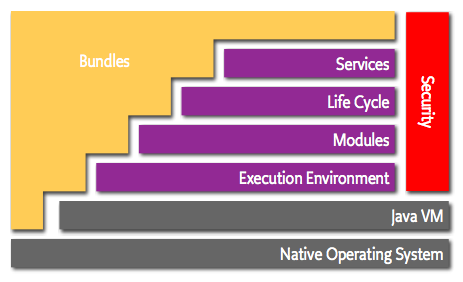
\includegraphics[width=0.8\textwidth]{images/Chapter_05/osgi-layering.png}
	\caption{OSGi layer structure}
	\label{fig:osgi-layering}
\end{figure}

\subsubsection{Bundles}
Bundles, also known as modules, are the smallest unit of modularization. Technically, they are a JAR file with additional meta information,
which are stored in a file called \textit{manifest file}. The manifest file is part of the standard Java specification, but OSGi adds additional
metadata to it in form of specific headers. The \textit{Bundle-SymbolicName} and the \textit{Bundle-Version} headers uniquely identify a
bundle. In OSGi is allowed to have bundles with same name, but different version running at the same time.

The manifest contains information like the bundle dependencies. A bundle can depend on another bundle or on a package. Preferred way
to define dependencies in a bundle is with \textit{Import-Package} and \textit{Export-Package} headers and not with \textit{Require-Bundle}
header. This gives you an access only to the packages that you need and allows you to exchange the packages at a later point in time

The OSGi runtime uses the information about the dependencies to \textit{wire} the bundles and hides everything in this JAR unless it is
explicitly exported. The dependencies to the Java standard libraries are managed by the \textit{Bundle-RequiredExecutionEnvironment}
header, so it is not needed to import the Java core packages

Bundles are used often to register and consume services.

\subsubsection{Lifecycle}
OSGi is a dynamic platform. That means that bundles may be installed, uninstalled, started, stopped or updated at runtime, as the table
\ref{table:bundle-states-description} indicates. The OSGi specification defines a mechanism how to manage the dependencies between
the bundles and the functionality that they provide. This is achieved with the help of the lifecycle concept.

The framework introduces a different states, transitions between these states and rules how this states are affecting the packages
exported by the bundle and the services, that it provides. The table \ref{table:bundle-states-description} shows the possible states
of an OSGi bundle with a short explanation

\begin{table}[]
	\centering
	\resizebox{\textwidth}{!}{%
		\begin{tabular}{|l|l|}
			\hline
			\multicolumn{1}{|c|}{\textbf{Status}} & \multicolumn{1}{c|}{\textbf{Description}}                                                                                                                                                                                                \\ \hline
			INSTALLED                             & \begin{tabular}[c]{@{}l@{}}The bundle has been installed into the OSGi container, but some of \\ it's dependencies are still not resolved. The bundle requires packages \\ that have not been exported by any other bundle.\end{tabular} \\ \hline
			RESOLVED                              & \begin{tabular}[c]{@{}l@{}}The bundle is installed and the all the dependencies at a class level \\ are resolved and wired. The bundle can export the packages, that it \\ provides.\end{tabular}                                        \\ \hline
			STARTING                              & \begin{tabular}[c]{@{}l@{}}A temporary state that the bundle goes through while the bundle is\\ starting, after all dependencies have been resolved. The bundle is \\ permitted to register services.\end{tabular}                       \\ \hline
			ACTIVE                                & The bundle is running                                                                                                                                                                                                                    \\ \hline
			STOPPING                              & \begin{tabular}[c]{@{}l@{}}A temporary state that the bundle goes through while the bundle \\ is stopping\end{tabular}                                                                                                                   \\ \hline
			UNINSTALLED                           & The bundle has been removed from the OSGi container                                                                                                                                                                                      \\ \hline
		\end{tabular}%
	}
	\caption{Bundle states description}
	\label{table:bundle-states-description}
\end{table}

The possible status transitions are shown in the state diagram in the figure \ref{fig:bundle-state-diagram}.

\begin{figure}
	\centering
	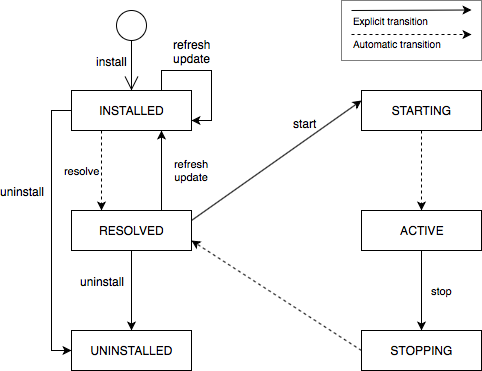
\includegraphics[width=0.8\textwidth]{images/Chapter_05/bundle-state-diagram.png}
	\caption{Bundle state diagram}
	\label{fig:bundle-state-diagram}
\end{figure}

\subsubsection{The Service Model}
The service model is another main concept that allows the bundles to communicate between each other.

In OSGi, a bundle can register a service in a central service registry under one or more service interface. Published services also
have service properties associated with them in the registry. It is an important feature of OSGi, because it provides a central place
to register and get services. A bundle is permitted to register service objects at any time during the STARTING, ACTIVE or STOPPING
states. Other bundles can go to the registry and list all objects, that are registered under a specific interface or class.

A bundle can therefore register a service, it can get a service and it can track for appearing and disappearing of service. Any
number of bundles can register the same service type and any number of bundles can get the same service. The figure \ref{fig:osgi-services}
represents a basic diagram of the service usage and tracking.

\begin{figure}
	\centering
	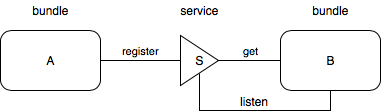
\includegraphics[width=0.7\textwidth]{images/Chapter_05/osgi-services.png}
	\caption{OSGi services \cite{osgiAlliance}}
	\label{fig:osgi-services}
\end{figure}

\subsubsection{Declarative Services}
In order to simplify the usage of services the OSGi Alliance has developed a model of managing services dynamically called Declarative
Services. It is based on three main concepts:

\begin{itemize}
	\item \textbf{Declarative Services Container (DS)}: a module that is managing the lifecycle of a service component dynamically.
	It activates and deactivated different components, basing its decisions on the information contained in the component description.
	\item \textbf{Service Component}: an object whose lifecycle is managed, usually by a component framework such as DS.
	\item \textbf{Component Description}: the declaration of a component, contained within an XML document in a bundle.
\end{itemize}

\paragraph{DS Container}
In order to use the Declarative Services, a bundle has to be started with an implementation of the DS container. In Equinox this
bundle is called \textit{org.eclipse.equinox.ds}.

When a bundle that contains a component is added to the framework, DS reads its component description and if the conditions
described in this file are fulfilled, the DS activates the component.

\paragraph{Components}
A component is a normal Java class, that can reference services and provide services. What makes it specific is that it is declared
in a XML file and is managed completely by the DS, so the DS instantiates the component, calls methods on it and manages its
lifecycle.

A component in a bundle requires an XML description of the component, a \textit{Service-Component} manifest header, which locates
the XML description, and an implementation class. There are three types of components:
\begin{itemize}
	\item \textbf{immediate}: with \textit{immediate} attribute set to true
	\item \textbf{delayed}: with \textit{immediate} attribute set to false
	\item \textbf{factory}
\end{itemize}

A component goes through several states in his lifecycle:
\begin{itemize}
	\item \textbf{UNSATISFIED}: initial state of the Service Component, after the bundle is started.
	\item \textbf{REGISTERED}: temporary state, only \textit{delayed} components go through this state.
	\item \textbf{ACTIVE}: the component is active and component instance is created.
\end{itemize}

\begin{figure}
	\centering
	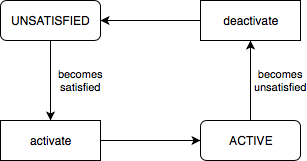
\includegraphics[width=0.6\textwidth]{images/Chapter_05/immediate-component-lifecycle.png}
	\caption{Immediate component lifecycle}
	\label{fig:immediate-component-lifecycle}
\end{figure}

\begin{figure}
	\centering
	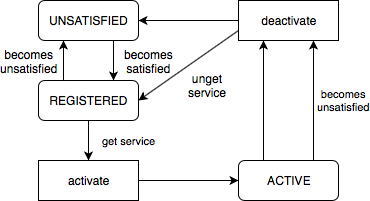
\includegraphics[width=0.6\textwidth]{images/Chapter_05/delayed-component-lifecycle.png}
	\caption{Delayed component lifecycle}
	\label{fig:delayed-component-lifecycle}
\end{figure}

The component lifecycle depends on the lifecycle of the bundle, that includes the component. Component must be enabled before it
can be used. A component is enabled, when the component's bundle is started and disabled, when the bundle is stopped.

After the Component is enabled, it is moved to the UNSATISFIED state. The next step is to satisfy the component configuration.

The component configuration is satisfied when:
\begin{itemize}
	\item Component is enabled.
	\item All the component references are satisfied. A reference is satisfied when the reference specifies optional cardinality or
	there is at least one target service for the reference. If the component has lazy initialization (the component is delayed), it is
	moved to the REGISTERED state and it is waiting to be activated, when the service is requested (see figure
	\ref{fig:delayed-component-lifecycle}).
	Otherwise (the component is immediate) as soon as its dependencies are satisfied, the component is activated (see figure
	\ref{fig:immediate-component-lifecycle}).
\end{itemize}

\bigskip
OpenHAB is much more than what we have explained in this chapter. But, as we will develop the project partially over openHAB,
we will explore more concepts from a developer perspective in the following chapter, like the installation of the system and the
configuration of its different parts.


\chapter{Project Development}
    
In each of the previous chapters I have explored different aspects of the fields of home automation and voice assistance from a 
theoretical point of view, from their definition to smaller details, including additional explanations about a specific home automation 
system, openHAB.

At this time, I think I have provided enough background to begin my case study: the building of a home automation controller. As I 
mentioned in the openHAB chapter, I will base my project on this system and build on it, as it accomplishes very well the main
requirements that I determined for this project.

In this chapter, I will detail the process that I have followed in order to develop this project, from its specification to the final result.

\section{Product Specification}
The first task to do is to define the product. What should a home automation system do? What do users expect it to do? How? All 
the answers to these questions can be clarified by following some processes that, although they do not completely answer them (we 
can see many failed projects from time to time), they provide a very clear and detailed specification from the beginning.

\subsection{Personas}
Creating personas is a common process applied to the product design and development process in order to help in making a user-centered
design, and it is applicable in this project in order to have a better idea of what would users expect from the final product.

A persona is a representation of a user, typically based off user research and incorporating user goals, needs, and interests.

In this project, I am going to use proto-personas, which are based on secondary research and the guess of who they should be designed 
for, as currently we do not have means and time for making true research-based personas (and it is not the main objective in this project).

After thinking about the main uses of this system and the people that would be interested on it, I have extracted these three personas, 
representing its main uses, although not the only ones. I have built them with the online platform Xtensio, and the figures
\ref{fig:persona-oswald-douglas}, \ref{fig:persona-anna-lahtinen} and \ref{fig:persona-rosario-vera} represent them. I tried to extract 
a varied range of backgrounds, current situations, desires and worries. 

Oswald Douglas (figure \ref{fig:persona-oswald-douglas}) is a freelance technology blogger from Dallas, USA, that is very interested 
in the areas of home automation and Internet of Things. He is looking to automate his own home and write about his experience in 
his blog. He already has experience with technology, and this next step will not be too difficult for him. His interests are clear: 
to try cutting-edge technology in his own home and make the most of home automation.

Anna Lahtinen (figure \ref{fig:persona-anna-lahtinen}) is a 16 year-old high school student from Lappeenranta, Finland. She is up 
to date on technology but she is not passionate about it. However, she heard about home automation and thinks that she could enjoy 
a better media experience with it. In addition, she thinks that adding smart color light bulbs to her bedroom would make it look more 
beautiful. However, she feels that there is a lack of general information about devices and the set up and configuration of a home 
automation system. She thinks that the price of it is too high as well.

Rosario Vera (figure \ref{fig:persona-rosario-vera}) is an administrative from Vitoria-Gasteiz, Spain. She is 37 years old, is married and 
has two young children. She is not very familiar with technology, but she has heard about home automation in the news and thinks 
that it could fit her needs. Rosario and her husband work outside home, and sometimes their children need to be alone at home. Home 
automation would provide more security to the home and would allow them to have more spare time. Voice assistance would be helpful 
for their children when they are alone, as it is a very easy and natural way to interact with technology. However, she is concerned about 
their privacy regarding these systems and she thinks that companies should give more accessible explanations about it. In addition, 
she finds these systems difficult to use.

\begin{sidewaysfigure}
    \centering
    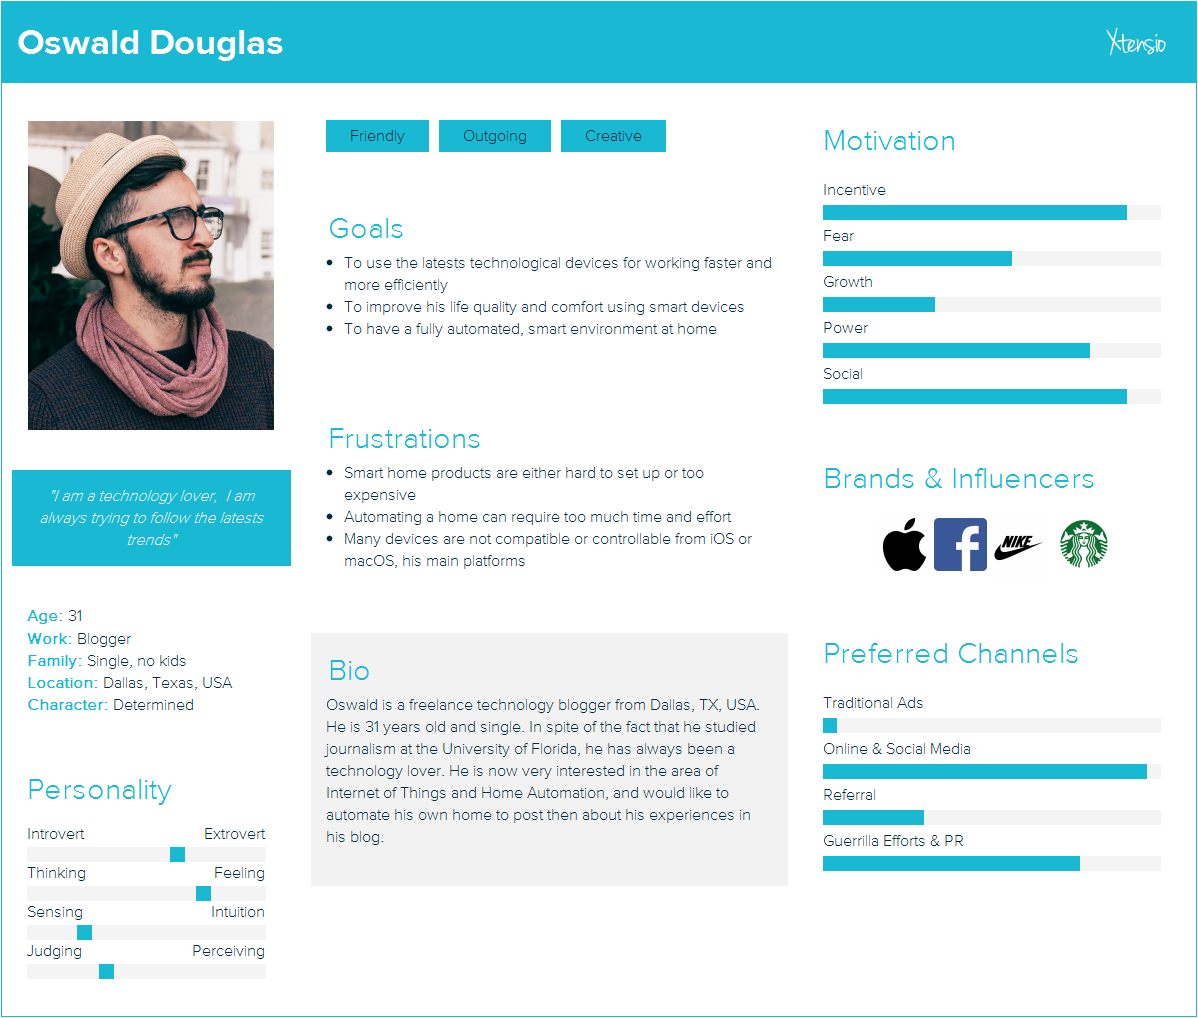
\includegraphics[width=0.65\textwidth]{images/Chapter_06/persona-oswald-douglas.png}
    \caption{Persona: Oswald Douglas}
    \label{fig:persona-oswald-douglas}
\end{sidewaysfigure}

\begin{sidewaysfigure}
    \centering
    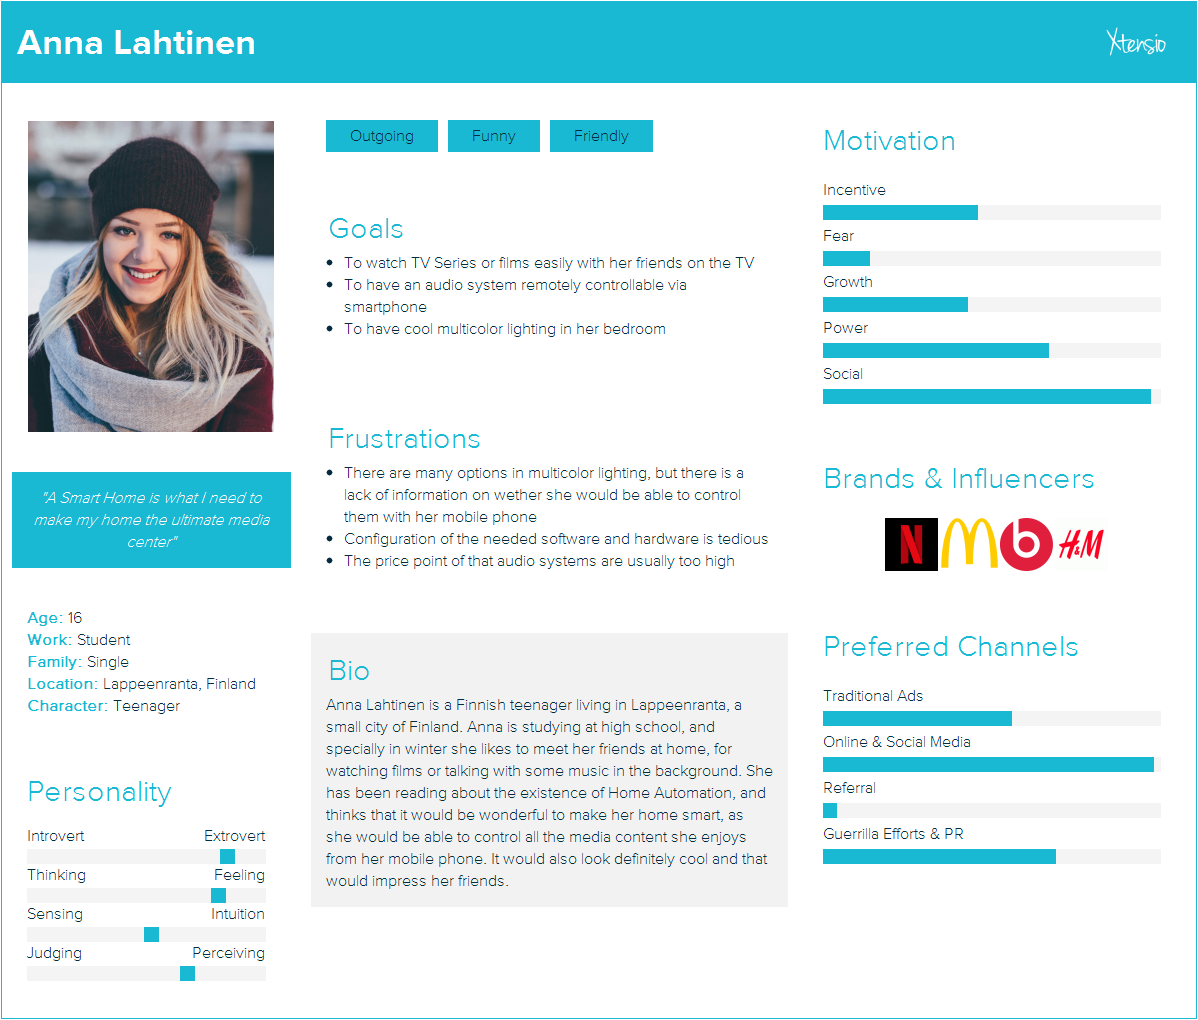
\includegraphics[width=0.65\textwidth]{images/Chapter_06/persona-anna-lahtinen.png}
    \caption{Persona: Anna Lahtinen}
    \label{fig:persona-anna-lahtinen}
\end{sidewaysfigure}

\begin{sidewaysfigure}
    \centering
    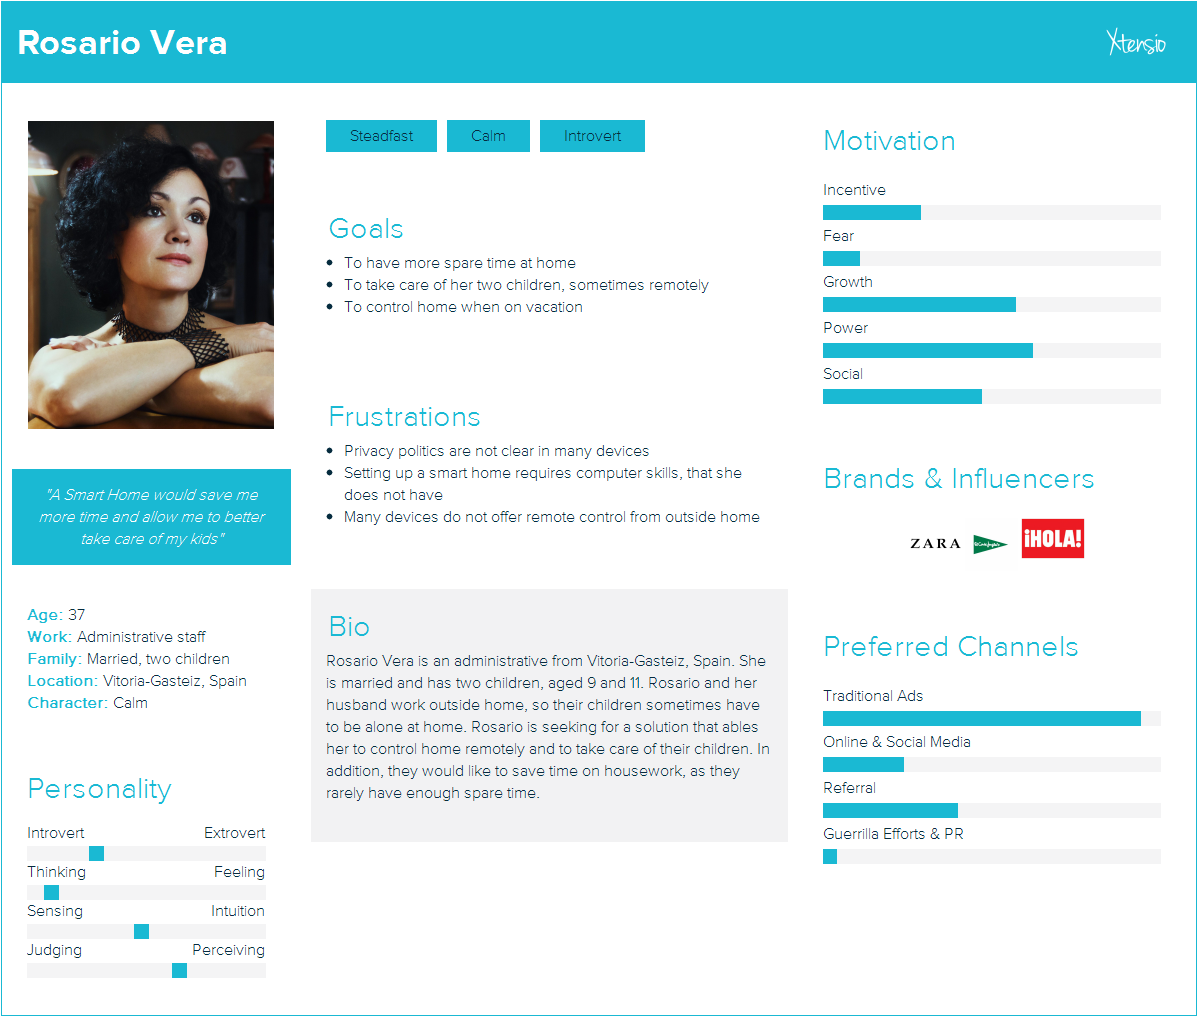
\includegraphics[width=0.65\textwidth]{images/Chapter_06/persona-rosario-vera.png}
    \caption{Persona: Rosario Vera}
    \label{fig:persona-rosario-vera}
\end{sidewaysfigure}

\subsection{Software Requirements Specification}
With the Software Requirements Specification (SRS), I try to describe the project to develop from a functional point of view, that is,
to determine the capabilities that the software system will have.

The domotic controller will be able to control all modern devices in our home, regardless of their maker and the technology they use.
It will provide an easy to use user interface and the ability to easily install, modify or remove the devices. It will also include natural
human-computer interaction through the voice. A more detailed specification of the requirements can be found in the subsections
below.

\subsubsection{Functional Requirements}
Functional requirements are a description of the facility or feature required. They deal with what the system should do or provide 
for users.\cite{sqaFunctionalNonFunctional}

\begin{itemize}
    \item \textbf{FR1}: The system will be able to retrieve automatically the status of the different properties of the elements.
    \item \textbf{FR2}: The system will be able to retrieve automatically data from its different data providers.
    \item \textbf{FR3}: The system will not need any operation to launch openHAB after it is powered on.
    \item \textbf{FR4}: The system will be able to turn itself off safely.
    \item \textbf{FR5}: The system will automatically detect new smart devices connected to the local network.
    \item \textbf{FR6}: The system will be able to detect the possible operations with each connected smart device. 
    \item \textbf{FR7}: The system will be able to operate with the connected devices according to the detected possible operations.
    \item \textbf{FR8}: The system will be able to tell the user in an understandable manner the current connection status for each
    device.
    \item \textbf{FR9}: The system will provide different user interfaces, so users can choose one between them, according to
    their needs.
    \item \textbf{FR10}: The user will be able to change the configuration of the system from a graphical user interface.
    \item \textbf{FR11}: The system will be manually configurable and modifiable using configuration files.
    \item \textbf{FR12}: The system will automatically include and configure new devices found in the network, after the user decides
    to add them.
    \item \textbf{FR13}: The user will be able to configure the name, display icon, IP and all possible aspects of the item directly from
    the user interface.
    \item \textbf{FR14}: The system will allow the user to make groups of items.
    \item \textbf{FR15}: The system will allow the user to add groups of items to other groups of items.
    \item \textbf{FR16}: The system will be modular and include a package system. Each package supports a set of devices.
    \item \textbf{FR17}: The package system will be accessible from the graphical user interface.
    \item \textbf{FR18}: The installation of packages will be done automatically after the user clicks on the install button.
    \item \textbf{FR19}: The removal of packages will be done automatically after the user clicks on the remove button.
    \item \textbf{FR20}: The system will maintain an updated and classified list of packages according to an external repository.
    \item \textbf{FR21}: The system will be manageable from external sources.
    \item \textbf{FR22}: The system will be accessible from external devices and from the Internet.
    \item \textbf{FR23}: The system will allow to have automation rules defined by the user.
    \item \textbf{FR24}: The voice assistant will allow to perform the main operations of each device in the system.
    \item \textbf{FR25}: The voice assistant will be able to answer in different languages.
    \item \textbf{FR26}: The voice assistant will be able to do power management tasks in the system, such as powering the system
    off or restarting the system.
    \item \textbf{FR27}: The voice assistant will be operable through mechanical methods or by voice.
    \item \textbf{FR28}: The users will be able to edit and adapt the functionalities of the voice assistant according to their needs.
    \item \textbf{FR29}: The voice assistant will provide spoken feedback if there has been an error performing the given command.
    \item \textbf{FR30}: The voice assistant will be able to print debug information in the command line if it is required.
\end{itemize}

\subsubsection{Non-Functional Requirements}
Non-functional requirements detail constraints, targets or control mechanisms for the new system. They describe how, how well or
to what standard a function should be provided.\cite{sqaFunctionalNonFunctional}

\begin{itemize}
    \item \textbf{NFR1}: The system, along with the voice assistant, will be installable in the Raspberry Pi.
    \item \textbf{NFR2}: The system and the voice assistant will provide a satisfactory response rate.
    \item \textbf{NFR3}: The user interfaces of the home automation system will be adaptable to the size and resolution of the
    user's screen.
    \item \textbf{NFR4}: The user interfaces will be made according to modern standards, like Material Design.
    \item \textbf{NFR5}: The home automation system will run in a local server, created in the machine which executes it.
    \item \textbf{NFR6}: In order to allow external connections, the home automation system will provide a REST API.
    \item \textbf{NFR7}: The system will provide secure access options.
    \item \textbf{NFR8}: The system must be available the 99\% of the time.
    \item \textbf{NFR9}: The system must be scalable.
    \item \textbf{NFR10}: The system must be recoverable in less than 45 minutes.
    \item \textbf{NFR11}: The cost of the system must me minimal.
    \item \textbf{NFR12}: The system must be interoperable with multiple devices.
    \item \textbf{NFR13}: The voice assistant will recognize English.
    \item \textbf{NFR14}: The voice assistant will be fast in its response. Therefore, its procedure for deciding a response will 
    be optimal.
    \item \textbf{NFR15}: The voice assistant will operate with the home automation system via REST, so it can be installed in a
    different computer than the one with the home assistant.
\end{itemize}

\subsection{Use Cases}
The next step after the specification of requirements is to specify the use cases of the system.

Use case diagrams are usually referred to as behavior diagrams used to describe a set of actions (use cases) that some system or 
systems (subject) should or can perform in collaboration with one or more external users of the system (actors).\cite{umlUseCaseDiagrams}

%TODO
%Hacer los diagramas de casos de uso tal y como indiqué en UC-device-and-service-control.xml
%Dividir los requisitos de modo que queden subsistemas funcionales diferenciados

\subsection{Functional Subsystems}
%TODO
%Especificar aquí los subsistemas funcionales

\subsection{Implementation Possibilities}
After exploring what users would expect from a system like this, it is worth thinking about how it should be implemented. Together 
with my director, I proposed different options to meet the previous requirements.

\subsubsection{Web Platform}
A well designed web platform is a great idea nowadays. If this platform is hosted in a local server, it means that it can be accessed
from any device connected to the network. With the correct configuration, it could be even reachable from anywhere in the world.
It is easy to implement and maintain, and users with basic web development knowledge would be able to easily modify it. In addition,
the same web platform can be adaptable to any device and resolution, thanks to responsive designs. It would also work if we attach
a tactile screen to the Raspberry Pi.

OpenHAB mounts a web platform in a local server by default, and provides several adaptable user interfaces, so this solution would
not require much effort, and it offers many possibilities.

\subsubsection{Desktop Application}
Another solution, focused on the Raspberry Pi desktop (where we mainly want to implement the system), is developing a desktop 
application with an adapted user interface for tactile screens. The advantage of a desktop application is that it usually requires 
less resources and it is faster, but it is a specific solution for the Raspberry Pi, so it would only work there. We would need a 
different application if we wanted it to run on mobile phones or tablets.

We would need to make it from scratch, as openHAB does not provide any desktop application.

\subsubsection{Mobile Application}
Mobile phones and \textit{tablets} are common devices that are widely used to manage smart homes. Some setups have a tablet located 
somewhere in the home, which is only used for managing the domotic devices. An application is faster and more accessible than a web
platform, and users are more used to them, so it would be convenient in some cases.

However, making the system only accessible from a mobile or tablet application would reduce the utility of the Raspberry Pi, and 
would at least require two devices (one for the local server and another one for accessing it). Although it is a good complement to the
system, it is not convenient to base it only on a mobile application. However, it is applicable in a hybrid solution.

\subsubsection{Hybrid Solution}
A hybrid solution consists of applying two or more solutions together of those specified above. For example, providing a web platform 
and an optional mobile application to easily manage the system from a mobile device.

OpenHAB provides a web platform, as explained above, and a mobile application for iOS and Android than connects to the web platform.

\subsubsection{Comparison}
The table \ref{table:possible-implementations} compares all the possibilities for the implementation of the system.

\begin{table}[]
    \centering
    \resizebox{\textwidth}{!}{%
        \begin{tabular}{|l|c|c|c|c|}
            \hline
            \multicolumn{1}{|c|}{\textbf{Feature}}                                  & \textbf{\begin{tabular}[c]{@{}c@{}}Web\\ platform\end{tabular}} & \textbf{\begin{tabular}[c]{@{}c@{}}Desktop \\ application\end{tabular}} & \textbf{\begin{tabular}[c]{@{}c@{}}Mobile\\ application\end{tabular}} & \textbf{\begin{tabular}[c]{@{}c@{}}Hybrid\\ Solution\end{tabular}} \\ \hline
            \begin{tabular}[c]{@{}l@{}}Support for \\ multiple devices\end{tabular} & Yes                                                             & Only PCs                                                                & \begin{tabular}[c]{@{}c@{}}Only mobile\\ phones/tablets\end{tabular}  & Yes                                                                \\ \hline
            \begin{tabular}[c]{@{}l@{}}Allows access\\ from Internet\end{tabular}   & Yes                                                             & No                                                                      & No                                                                    & Yes                                                                \\ \hline
            \begin{tabular}[c]{@{}l@{}}Control from\\ Raspberry Pi\end{tabular}     & Yes                                                             & Yes                                                                     & No                                                                    & Yes                                                                \\ \hline
            \begin{tabular}[c]{@{}l@{}}Easy \\ implementation\end{tabular}          & Yes                                                             & No                                                                      & No                                                                    & Yes                                                                \\ \hline
            \begin{tabular}[c]{@{}l@{}}Maximum\\ performance\end{tabular}           & No                                                              & Yes                                                                     & Yes                                                                   & Partially                                                          \\ \hline
        \end{tabular}%
    }
    \caption{Comparison between possible implementations}
    \label{table:possible-implementations}
\end{table}

As we can see, the hybrid solution, which is a web platform and mobile application, meets all the features in the best way, and 
offers easy and fast implementation. At this point, I have not considered the implementation of the voice assistant, which I will 
talk about in following sections.

\bigskip
\section{System Analysis}
%TODO
%Introducir la sección

\subsection{Conceptual Model}
%TODO
%Especificar el modelo conceptual

\bigskip
\section{System Design}
%TODO
%Introducir la seccion

\subsection{Architecture}
%TODO
%Especificar la arquitectura del sistema, se puede hacer una explicacion rapida de los subsistemas que lo componen

\subsection{Conceptual Class Diagram}
%TODO
%Introducir y especificar el DCC

\bigskip
\section{Implementation}
In this section, I will explain the process that I have followed to implement the home automation controller, along with the voice
assistant.

\begin{figure}
    \centering
    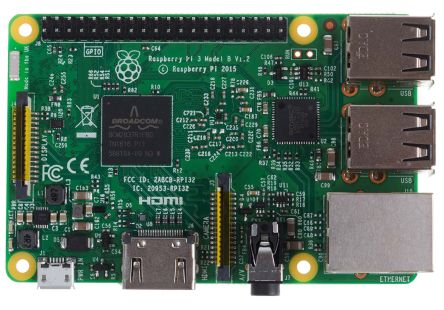
\includegraphics[width=0.8\textwidth]{images/Chapter_06/raspberry-pi-3b.jpg}
    \caption{Raspberry Pi 3 Model B}
    \label{fig:raspberry-pi-3b}
\end{figure}

As I have mentioned before, the main objective is to install the system in a Raspberry Pi, which is an affordable and small computer,
with enough power and connectivity options to install a home automation system on it, and even a voice assistant. The possibilities 
of this device are endless: it can work with or without display, and has a special connector to which the user can connect screens, 
microphones, speakers and many other accessories. It also has USB ports on its high-end models, and accepts all the USB 
accessories that a normal computer would accept.\cite{raspberryPiDocs}

The first approach to this system was to install Raspbian, a Linux distribution provided by openHAB, over a Raspberry Pi 3 Model B 
(figure \ref{fig:raspberry-pi-3b}). Raspbian has openHAB preinstalled and configured, so it is ready to use. The first idea was to 
have a computer with openHAB and then a voice assistant in other machine. I installed the distribution on this mini PC, but after 
reviewing the possible voice assistants, I found that it was not the best way to implement it. 

I found the Google AIY Voice Kit, which is a kit provided by Google to makers that want to play around with voice recognition.
They provide a package with some accessories for the Raspberry Pi and a cardboard box that is meant to contain the board and the
accessories. Then, I reconsidered the architecture. It would be also possible to install openHAB in the same machine as the virtual
assistant. This way, we would need just one machine for all. It would be a voice assistant, but with a local server, accessible from
all the devices connected to the local network. It would be possible to attach a screen to it as well, so the user can manage the
smart home graphically from the same device.

I thought this would be the best solution, and it would still meet all the requirements specified previously. So, I began working on it.

\subsection{Introduction to Google AIY Voice Kit}
The AIY Voice Kit is a do-it-yourself project created by Google that demonstrates how easy and inexpensive can be to create a natural 
voice recognizer that works with Google Assistant, at a price of only EUR 30 in Europe. The project, aimed for makers, also lets the 
user add their own questions, which is the most powerful part for our purpose. 

The idea is to adapt the device in order to fetch the voice commands that the microphone captures and manage them in openHAB, 
making the system act following user’s instructions.

\subsubsection{Capabilities}
The main advantage of the Google AIY Voice Kit, and the reason why we have chosen it for this project, is that we can access the 
Google Cloud Voice API and create our own voice interfaces. Everything is coded in Python, and we can create voice commands to 
control it.

This, along with the more than reasonable quality of its stereo microphone and speaker, make it a very useful device that could 
perfectly fit in a smart home, despite its looks.

The device is capable of recognizing the “OK Google” command, as well triggering the assistant when the big red button is pressed, 
and, by default, it is capable of doing almost everything that the Google Assistant on smartphones can do, including integration 
with the apps in the user’s smartphone and reading the news, among other things.

\subsubsection{The Main Challenge}
The challenge is to explore how Google AIY Voice Kit and openHAB 2, both installed on the same system, can work together and, 
if it is possible, connect them so a standard user can control its smart home using voice commands and universal, open source solutions.

\subsection{Building the Google AIY Voice Kit}
For making the voice recognizer, I primarily used:

\begin{itemize}
    \item Cardboard for the body of the device.
    \item A speaker.
    \item A Voice HAT microphone board and an accessory board.
    \item A big button with a light inside to trigger the voice recognition.
    \item A Raspberry Pi Model 3 B.
    \item An 8GB microSD card.
    \item Cables to connect everything.
\end{itemize}

\begin{figure}
    \centering
    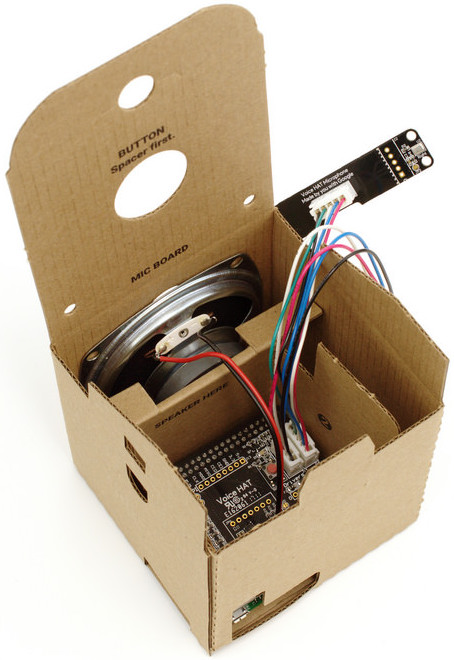
\includegraphics[width=0.5\textwidth]{images/Chapter_06/aiy-voice-kit.jpeg}
    \caption{The AIY Voice Kit}
    \label{fig:aiy-voice-kit}
\end{figure}

First of all, I had to put all the items together and assemble the cardboard body. The Voice HAT accessory board is connected to the 
Raspberry Pi through its GPIO connector, which is adapted to connect the rest of devices: the speaker, the microphone board and the
button. Once everything was correctly connected, I had to assemble the cardboard body, which was composed by two 
pieces.\cite{aiyProjectsVoice}

The next step was to write the Voice Kit SD image\cite{voiceKitSdImage} to the microSD card. I used the \textit{Etcher.io} macOS 
application for this purpose. 

The system includes everything that the Raspberry Pi needs to use the connected devices, so I only needed to check that they worked 
fine and were correctly connected. The system also includes two demos with Google Assistant: one that triggers the assistant by saying 
“OK Google!”, and another that needs the button to be pressed to trigger it.

To make any demo or a new app that uses Google Assistant work, it is necessary to register a new project on Google Cloud Platform 
(GCP) first. A project of this kind has to include the Google Assistant API, which can be enabled via GCP, as well as an OAuth 2.0 
client. Finally, at the moment of running the application, it seeks a JSON file that contains all this information. By default, it 
must be placed in the home folder and it must be called assistant.json.

Google Assistant gathers all the user’s information from their Google account, so they must have enabled the web and app activity, 
the device information and the voice and audio activity from their Activity Controls panel in their Google account settings.

\subsection{Setting up openHAB 2}
In this case, the goal is to install openHAB in the Linux distribution that the AIY Kit provides, which is a fork of Raspbian 
(that is a fork of Debian made for the Raspberry Pi), with the suitable drivers in order to support all the accessories from the kit. 
Luckily, openHAB provide in their documentation pages\cite{openHABDocs} enough instructions to make this process easier.

In this process, I used a keyboard and a mouse for interacting with the operating system, but it can also be done remotely via 
SSH connection.

As a prerequisite, Java 8 must be installed on the system. Users may prefer Zulu, the main Java \textit{alternative}, a fully 
certified build of OpenJDK.\cite{zuluWebsite}

OpenHAB 2 can be installed though a package repository or manually from file, but it is recommended to install through a package
repository, using \textit{apt}, \textit{apt-get}, \textit{yum} or \textit{dnf}. As this operating system is based on Debian, I used 
\textit{apt-get}.

First of all, I have to add the openHAB 2 Bintray repository key to the package manager and allow \textit{apt} to use the HTTPS 
Protocol.

\begin{lstlisting}[style=Consola]
wget -qO - 'https://bintray.com/user/downloadSubjectPublicKey?username=openhab' | sudo apt-key add - 
sudo apt-get install apt-transport-https
\end{lstlisting}

OpenHAB offers Stable (Official), Beta and Snapshot builds to choose from. The stable builds contain the latest official release 
with tested features, so it is the \textit{safest} to use. I will install this one. Then, I need to add the openHAB 2 Stable Repository 
to your systems apt sources list

\begin{lstlisting}[style=Consola]
echo 'deb https://dl.bintray.com/openhab/apt-repo2 stable main' | sudo tee /etc/apt/sources.list.d/openhab2.list
\end{lstlisting}

Next, I have to resynchronize the package index:

\begin{lstlisting}[style=Consola]
sudo apt-get update
\end{lstlisting}

And now I can install openHAB:

\begin{lstlisting}[style=Consola]
sudo apt-get install openhab2
\end{lstlisting}

Optionally, it is possible to install the add-ons package (\textit{openhab2-addons}), but it is meant to be installed if the machine 
is going to be disconnected from the Internet, as openHAB downloads them on request by default. In this case, I assume that the
system is going to be connected to Internet always.

At this point, I can start openHAB and register it to be automatically executed at system startup. To this end, the documentation 
provides the following commands for systems based on \textit{systemd}, such as Raspbian.

\begin{lstlisting}[style=Consola]
sudo systemctl start openhab2.service
sudo systemctl status openhab2.service

sudo systemctl daemon-reload
sudo systemctl enable openhab2.service
\end{lstlisting}

After some minutes, openHAB is ready on the local server, in the port 8080 (accessible in http://localhost:8080). Then, the following
commands are used to control the service.

\begin{figure}
    \centering
    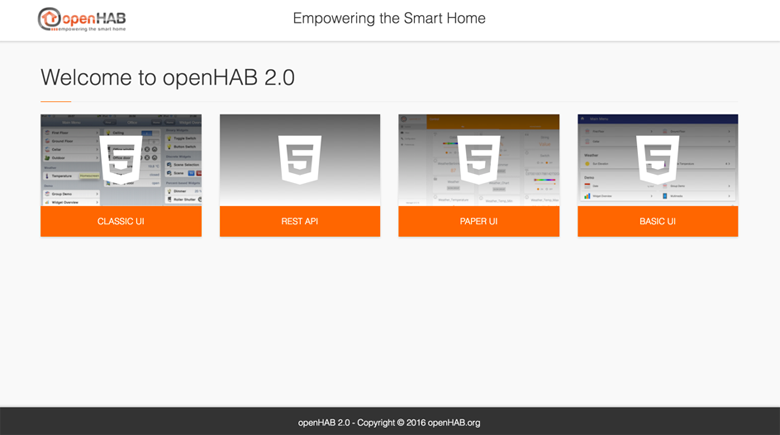
\includegraphics[width=1\textwidth]{images/Chapter_06/openhab-startup.png}
    \caption{OpenHAB 2 startup screen}
    \label{fig:openhab-startup}
\end{figure}

\begin{lstlisting}[style=Consola]
# Current service status
sudo /etc/init.d/openhab2 status

# (Re-)Start openHAB (background service)
sudo /etc/init.d/openhab2 restart

# Stop the openHAB background service
sudo /etc/init.d/openhab2 stop

# Make openHAB automatically start after booting the Linux host
sudo update-rc.d openhab2 defaults
\end{lstlisting}

OpenHAB installs also a utility in the command line interface, named \textit{openhab-cli}, that provides access to the openHAB-specific 
commands.

\begin{lstlisting}[style=Consola]
Usage:  openhab-cli command [options]

Possible commands:
  start [--debug]     -- Starts openHAB in the terminal.
  stop                -- Stops any running instance of openHAB.
  status              -- Checks to see if openHAB is running.
  console             -- Opens the openHAB console.
  backup [filename]   -- Stores the current configuration of openHAB.
  restore filename    -- Restores the openHAB configuration from a backup.
  showlogs            -- Displays the log messages of openHAB.
  info                -- Displays distribution information.
\end{lstlisting}

Lastly, to stay up to date to new releases, they recommend to execute the following commands periodically. Note that this also applies
to the rest of the packages installed in the Linux system.

\begin{lstlisting}[style=Consola]
sudo apt-get update
sudo apt-get upgrade
\end{lstlisting}

\subsection{Adding Philips Hue Devices}
Now that we have openHAB 2 up and running in the Raspberry Pi integrated in the AIY Kit, it is desirable to add a device to the home 
automation system. We have a Philips Hue lightning system available, so in this section I will explain the process that we have followed
to add it and configure it in our openHAB 2 instance.

\subsubsection{The Hue System}
Our Philips Hue system is composed by the \textit{white and color ambiance starter kit}\cite{philipsHueMeethue} (which consists 
in three Hue white and color lights and a Hue hub) as well as a Hue motion sensor:

\begin{itemize}
    \item \textbf{The Hue Hub} acts as a bridge between the user interface (the smartphone application or the OpenHab instance) and 
    the connected devices. It is configured and controlled via the Hue app and supports up to 50 lights at the same time. It communicates 
    via Zigbee with the Hue devices.
    \item \textbf{The Hue Motion Sensor} can be configured to turn on and off the lights when it detects movement and under some 
    defined conditions. By default, it is configured from the Hue app.
    \item \textbf{The Hue White and Color Lights} are customizable RGB lights. By default, they are configurable from the Hue app, 
    which offers many ways of changing the light emission.
\end{itemize}

\subsubsection{Installation and Configuration Process on PaperUI}
Philips, as many other companies, is restrictive regarding their home automation devices, and every communication between the Hue 
devices and the controller (openHAB in this case) needs to pass through the Hue Hub. The Hub communicates via WiFi with the controller 
and via Zigbee with the Hue devices. The software it uses is privative, but luckily openHAB 2 implements protocols that make possible 
the communication between the controller and the Hub. This makes the Hub, though, a frustrating addition to our home automation system.

The Hue system needs to be configured from the Philips Hue mobile application in the first place. This process will link the Hub with the 
desired Hue devices, so the next time that the user connects to the Hub, it will not be necessary to configure them again, even if 
the connection is done from openHAB. The application allows to manage rooms and sort the devices, as well as setting automated commands 
(for instance, turning the light on when the motion sensor detects any movement). OpenHAB is unable to perform such complex operations 
by default, providing only a few channels for the light bulb.

Once the Hub is on, connected and linked with the Hue devices, we can proceed to configure it on openHAB. In this case, I explain 
the process to follow in order to add the light bulb controls, but it might work for other Hue devices in a future. If openHAB is 
used on a system connected to the same network as the Hub, the Hub will automatically appear in the \textit{Inbox} section. We have 
to make sure before that its related binding. Adding the Hub in the Inbox section means that it will be listed as a Thing. OpenHAB 
takes care automatically of the Thing (figure \ref{fig:philips-hue-hub-thing}) and Items configuration. After adding them, the host 
device and the Hub will be able to communicate between them. However, the user needs to press the pairing button on the Hub in 
order to activate the communication.

\begin{figure}
    \centering
    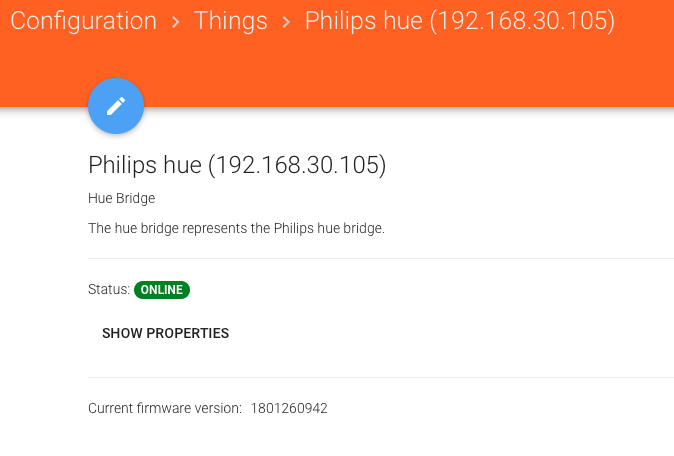
\includegraphics[width=0.9\textwidth]{images/Chapter_06/philips-hue-hub-thing.png}
    \caption{Philips Hue Hub Thing}
    \label{fig:philips-hue-hub-thing}
\end{figure}

After that, the Hub will act as a bridge and openHAB will be able to display all the compatible devices connected to the Hub. In 
this case, the Hue color lamp appears in the Inbox. The process for adding it is the same as with the Hub. Nevertheless, this time 
the light controls will be added automatically to the Control panel according to the linked channels on the thing. OpenHAB supports 
two channels that are directly related to the bulb functionality: \textit{color} (which is divided in tone, brightness and saturation) 
and \textit{white temperature}. The first one will set the light in a color with the desired properties, and the second will set a 
white color from a range of whites (from cold to warm white). Additionally, OpenHAB provides two more channels: \textit{alert}, 
to use the bulb as an alert light under certain circumstances, and \textit{color loop}, which will make the light color iterate in 
the whole color spectrum. The figure \ref{fig:hue-color-bulb-channels} shows the PaperUI interface showing these channels.

\begin{figure}
    \centering
    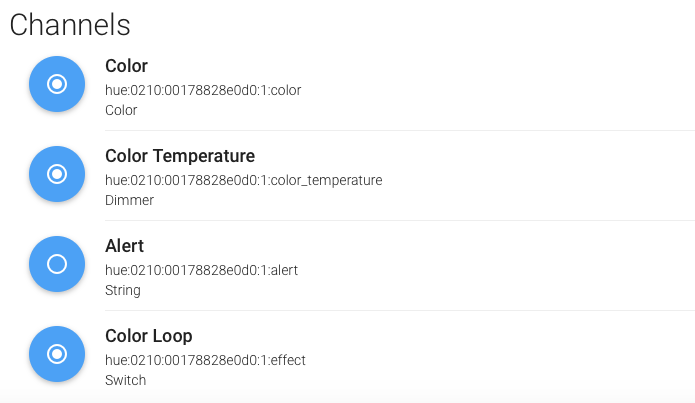
\includegraphics[width=0.9\textwidth]{images/Chapter_06/hue-color-bulb-channels.png}
    \caption{Available channels in the Hue color bulb}
    \label{fig:hue-color-bulb-channels}
\end{figure}

\begin{figure}
    \centering
    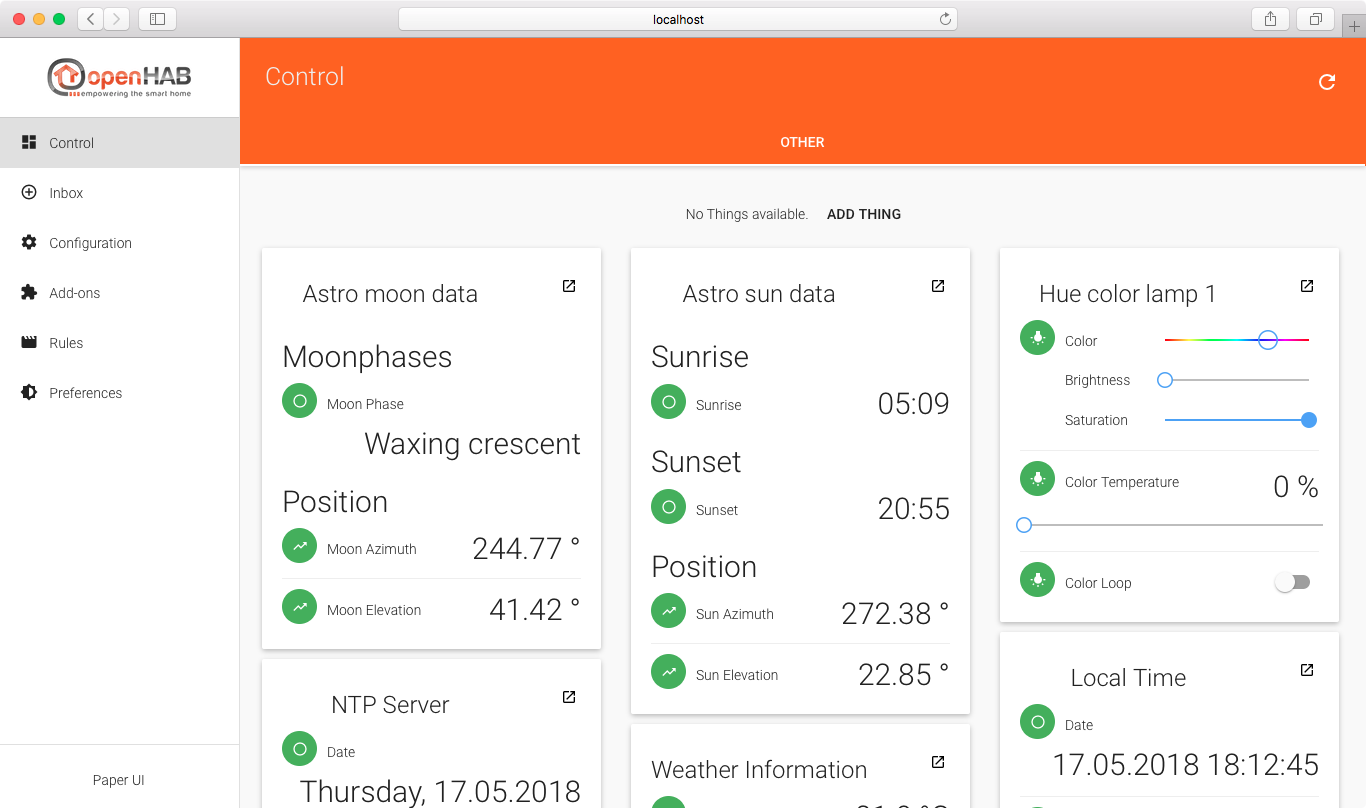
\includegraphics[width=1\textwidth]{images/Chapter_06/openhab-control-hue.png}
    \caption{OpenHAB 2 Control Panel with the Hue color bulb controls}
    \label{fig:openhab-control-hue}
\end{figure}

\subsubsection{Internal Functionality}
OpenHAB is able to communicate with the Hue Hub and Hue devices thanks to the Philips Hue binding (represented as a set of packages 
in Java, as shown in the figure \ref{fig:hue-binding-structure}), integrated in the Eclipse SmartHome Extensions repository. 

\begin{figure}
    \centering
    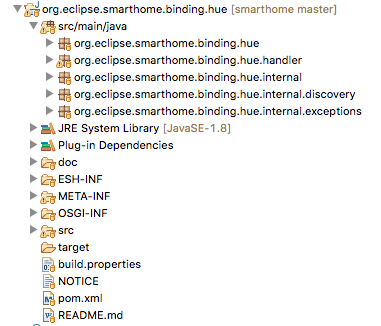
\includegraphics[width=0.6\textwidth]{images/Chapter_06/hue-binding-structure.png}
    \caption{Philips Hue binding internal structure}
    \label{fig:hue-binding-structure}
\end{figure}

As we can see, there are packages for handling the lights and Hub (which is named \textit{bridge}), and for managing the internal 
functionality of the binding and openHAB. That is, discovering the devices and showing them in the Inbox and managing exceptions. 
Examples of exceptions can be having the device off or sending the device a wrong command.

Looking more closely at the device handlers, we can see that the bridge handler implements a \textit{Runnable} object with a 
\textit{run} method, which gets the Hub configuration. The function gets the IDs of all the lights connected to the Hub and iterates 
over them. If a light is not listed in a list of light states caught from openHAB, it is added as a new light. If it is listed, then 
it checks for changes in the status of the light, comparing the actual state with the last one saved. If the states are different, 
notifies the Light listeners. There is a \textit{LightStatusListener} interface that is called on each change, it will modify the 
Light and Hue objects.

\subsection{Specifying Items Manually}
In previous chapters, I introduced the concept of Item in openHAB 2. Items represent functionalities that can be used by the 
applications, mainly user interfaces or automation logic.

OpenHAB is able to configure many Things and Items automatically in the PaperUI. But in many cases we may need to specify Items
manually. For example, for creating custom views(sitemaps), as we will see below. Therefore, it is important to know how to specify
Items manually.

First of all, I need to create an Items file. Both the items and the sitemap files are located in the \$OPENHAB\_CONF directory, 
which is different on different operating systems. In my case, they are located in:

\begin{lstlisting}[style=Consola]
/usr/share/openhab2/conf/items       <-- *.items files
/usr/share/openhab2/conf/sitemaps    <-- *.sitemap files
\end{lstlisting}

After a fresh installation these directories are empty (except for the \textit{readme} files), so I have to create a file there.
I will call it \textit{default.items}.

OpenHAB has its own syntax for defining Items and Sitemaps, but it is very easy to use. The basic syntax for defining an item is:

\begin{lstlisting}[style=Consola]
ItemType ItemName "ItemDescription" <ItemIcon> {ItemToThingChannelLink}
\end{lstlisting}

The code I have used for defining the item linked to the color channel and the item linked to the white tone channel of a Philips 
Hue color bulb is the following:

\begin{lstlisting}[style=Consola]
Color HueColor1 "Hue Light Bulb 1 Color" <lightbulb> {channel="hue:0210:00178828e0d0:1:color"}

Dimmer HueDimmer1 "Hue Light Bulb 1 Temperature" <lightbulb> {channel="hue:0210:00178828e0d0:1:color_temperature"}
\end{lstlisting}

Now, these Items are registered in the system, but before we can see them, I have to define a sitemap and include them there.

\subsection{Creating a Sitemap}
PaperUI, the newest addition in openHAB 2, is meant to make easier the device management, configuration and discovery. Many of 
these processes are carried out seamlessly, without user intervention. But this user interface lacks some functionalities, such as
custom ordering of Things. \textit{Sitemaps} are custom views that can be displayed in another user interface, the Basic UI, which
is also automatically installed at the beginning.\cite{openHABDocs} Sitemaps take defined Items and display them as the user specifies 
in the UI.

The user is able to define as many sitemaps as desired, and they can be selected from openHAB 2 home screen, in the Basic UI. Sitemaps 
are text files with the .sitemap extension, and they are defined in the folder thet I specified in the previous section, inside the openHAB 
installation directory.

The basic syntax that a sitemap follows is:

\begin{lstlisting}[style=Consola]
sitemap <sitemapname> label="<title of the main screen>" 
{
    [all sitemap elements]
}
\end{lstlisting}

Sitemaps are composed by arranging various user interface elements. A set of different element types supports a user-friendly and 
clear presentation. One line of Sitemap element definition produces one corresponding UI element. As shown in the example on the
figure \ref{fig:hue-bulb-sitemap}, each element generates a descriptive text next to an icon on the left side and a status and/or 
interaction elements on the right.

A certain set of parameters can be configured to customize the presentation of an element. In the shown example \textit{item} and 
\textit{icon} are parameters. Almost all parameters are optional, some are however needed to result in a meaningful user interface. 

By encapsulating elements with curly brackets, multiple elements can be nested inside or behind others. The Frame element type is 
often used in combination with element blocks. Frames are used to visually distinguish multiple elements of the same topic on one 
interface page. When using code blocks behind other element types such as \textit{Text}, \textit{Group} or \textit{Switch}, these UI 
elements will, in addition to their normal function, be links to a new view, presenting the nested elements. In the example in 
\ref{fig:hue-bulb-sitemap}, I created a single Frame that represented all the functionalities of the Hue Color Light.

The \textit{sitemap} element is mandatory in a Sitemap definition. This element shall be the first line in the sitemap file, and the 
following code block comprises the entire Sitemap definition.\cite{openHABDocs}

\begin{figure}
    \centering
    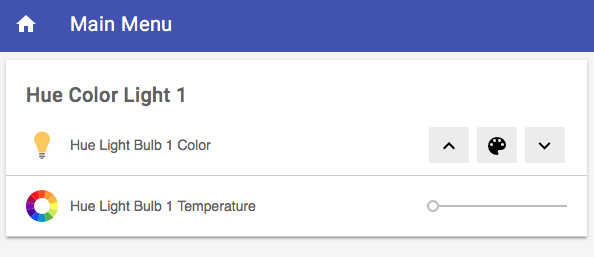
\includegraphics[width=0.9\textwidth]{images/Chapter_06/hue-bulb-sitemap.png}
    \caption{Basic UI displaying a Hue Color Light Item}
    \label{fig:hue-bulb-sitemap}
\end{figure}

From the previous example, I built a sitemap that could display the Hue color light Item that I configured previously in the Basic UI.
The figure \ref{fig:hue-bulb-sitemap} shows the result of introducing the following code in a file that I called \textit{default.sitemap}.

\begin{lstlisting}[style=Consola]
sitemap demo label="Main Menu"
{
    Frame label="Hue Color Light 1" {
        Colorpicker item=HueColor1 icon="slider"
        Slider item=HueDimmer1 icon="colorwheel"
    }
}
\end{lstlisting}

A frame is containing the main functionality of the Hue color light bulb, and that can be done for every new component installed at home.

OpenHAB 2 allows us to group our items so we can sort them by room or type. That can be made through the Group Item type.

\subsubsection{Elements on a Sitemap}
The element types specified in the table \ref{table:openhab-sitemaps-types} may be used in a Sitemap definition file.

\begin{table}[]
    \centering
    \resizebox{\textwidth}{!}{%
        \begin{tabular}{|l|l|}
            \hline
            \multicolumn{1}{|c|}{\textbf{Type}} & \multicolumn{1}{c|}{\textbf{Description}} \\ \hline
            Chart & Adds a time-series chart object for persisted data \\ \hline
            Colorpicker & Allows the user to choose a color from a color wheel \\ \hline
            Default & \begin{tabular}[c]{@{}l@{}}Renders an Item in the default UI representation specified \\ by the type of the given Item\end{tabular} \\ \hline
            Frame & \begin{tabular}[c]{@{}l@{}}Establishes an area containing various other Sitemap \\ elements\end{tabular} \\ \hline
            Group & \begin{tabular}[c]{@{}l@{}}Concentrates all elements of a given group in a nested \\ block\end{tabular} \\ \hline
            Image & Renders an image given by an URL \\ \hline
            Mapview & Displays an OSM map based on a given Location Item \\ \hline
            Selection & \begin{tabular}[c]{@{}l@{}}Provides a dropdown or modal popup presenting values\\ to choose from for an Item\end{tabular} \\ \hline
            Setpoint & \begin{tabular}[c]{@{}l@{}}Renders a value between an increase and a decrease \\ buttons\end{tabular} \\ \hline
            Slider & Presents a value in a progress-bar-like slider \\ \hline
            Switch & Renders an Item as an ON/OFF or multi-button switch \\ \hline
            Text & Renders an Item as text \\ \hline
            Video & Displays a video stream, given a direct URL \\ \hline
            Webview & Displays the content of a webpage \\ \hline
        \end{tabular}%
    }
    \caption{Types of elements for a Sitemap in openHAB 2}
    \label{table:openhab-sitemaps-types}
\end{table}

Data presented by Sitemap elements will almost always originate from a referenced Item. Each Item is of a certain Item type, for 
example \textit{Switch}, \textit{Number} or \textit{String}.

While not all combinations are meaningful, Items of one \textit{datatype} may be linked to different Sitemap element types. This 
provides the flexibility to present Items in the way desired in the home automation user interface.

\bigskip
At this point, I have openHAB installed in the Raspberry Pi inside the AIY Voice Kit. OpenHAB is communicating with the Hue Hub and
the Hue Color Light, and its state can be changed by accessing to the server that openHAB has created in the local network. This means
that, if I type on the browser of my mobile phone the IP address of openHAB and its port (8080), I will be able to control the light from
my phone as well. The state of the bulb can be changed from PaperUI (with the view that it has generated automatically) and from 
Basic UI, with the view and Items that I have specified in these previous steps.

Now the challenge is to build an assistant that can communicate with openHAB, and that is able to change the state of the configured
Items.

\subsection{Voice Assistants and Speech-To-Text Services}
The Google AIY Voice Kit, the device I am building the system on, already provides some files to access the Google Assistant. This
means that, by default, it can work just like any Google Home device (I explored these devices in previous chapters), so it can
provide general information and knowledge, play songs and tell the weather forecast, among other things. The files that the AIY Voice
Kit provide are accessible and modifiable, so I could write an assistant that would work on top of the Google Assistant, with special
commands.

\subsubsection{Introduction}
We could divide a simple voice assistant, like the one I am building on top of the Google Assistant for managing openHAB and the 
Raspberry Pi, in three different parts:
\begin{enumerate}
    \item Speech-To-Text (STT) conversion.
    \item Command processing.
    \item Text-To-Speech (TTS) conversion.
\end{enumerate}

The flow after each command from the user follows the order above. On the next few lines, I am going to explain a little further 
each one of these points.

\subsubsection{Speech-To-Text}
The Speech-To-Text or STT comes from the Speech Recognition, a sub-field of computational linguistics and IA. It is a computer 
technique that enables the recognition and transcription of spoken language into text by analyzing the captured audio.

It is the first step on the machine after capturing the voice, and it requires the execution of complex algorithms. This is why many 
companies, like Google, offer “cloud speech recognition”, where the audio is entirely processed in the cloud, taking advantage of 
very powerful computers. Thanks to this, its precision is much higher than other local solutions.

\subsubsection{Command Processing}
Once the system has the transcription of the spoken command, it must relate it with an action. It can be the execution of a function, 
or just a spoken response, or both. The complexity of this part can vary significantly, depending on the range of actions we would 
like the assistant to perform, or on how specific we want to be when recognizing the language.

There are grammar specifications and even XML dialects for this purpose, like AIML. For the custom assistant I have built, I also 
propose a model for processing the speech, as I will mention in further sections.

\subsubsection{Text-To-Speech}
Text-To-Speech or TTS is the inverse process of STT, that is, the artificial production of human speech given a text through a 
number of processes that produce a pronounceable version of the text and a digital sound, thanks to signal treatment techniques.

It is often the final step in the interaction with an assistant, when the assistant gives a response to a command given by the user.

\subsubsection{STT and TTS in the Custom Assistant}
The part where I have researched the most, which is also the one that offers more possibilities to this kind of assistant, is the 
speech recognition. I have found plenty of services that offer this technology, locally and in the cloud. Many of them work on 
Raspberry Pi, the heart of the Google AIY Kit.

Google integrates in this kit the integration with two STT services: the Google Assistant Library and the Google Cloud 
Speech-To-Text API\cite{googleCloudSttWebsite}. Both of them make the transcription in the cloud, freeing the Raspberry Pi from 
using much processing power in it. Both of them are truly accurate and rarely produce a wrong result, as it is expected from Google. 
Using this implementation of the Google Assistant Library is free, but it only works in English at this moment, so it is only 
possible to make the assistant in this language with this service. On the other hand, the Google Cloud Speech API is capable of 
recognizing more than 120 languages with its variants, even with long audio files. It can also provide content filters and automatic 
punctuation. But this solution is not totally free, it comes with a price of \$0.006 USD per 15 seconds of audio after 60 minutes, 
each month.\cite{craftworkzBlog}\cite{globalmeBlog}

Outside of Google, there are many other services that could also work with our assistant, from local solutions like 
CMUSphinx\cite{cmusphinxWiki} to cloud services provided by other companies. Local solutions offer offline recognition, in 
exchange for taking up large storage space and being slower and a lot more inaccurate than the cloud ones. Furthermore, 
cloud services are constantly updated and offer state-of-the-art voice recognition. They are usually very fast and, as they work 
in the cloud, do not need space on the user's drive. Usually, the providers of these services are major technology companies 
such as Microsoft and IBM\cite{ibmWatsonSttWebsite}, which provide the API for a periodic fee.

To find out which service best fits in my custom assistant, I compare the most interesting ones I have found in the table 
\ref{table:comparison-stt-services}.

\begin{table}[]
    \centering
    \resizebox{\textwidth}{!}{%
        \begin{tabular}{|l|l|l|l|l|}
            \hline
            \textbf{Name} & Assistant Library & Cloud TTS\cite{googleCloudSttWebsite} & Pocketsphinx\cite{cmusphinxWiki} & Watson STT\cite{ibmWatsonSttWebsite}\cite{ibmDeveloperWorksRecipes} \\ \hline
            \textbf{Maker} & Google & Google & CMUSphinx & IBM \\ \hline
            \textbf{Location} & Cloud & Cloud & Local & Cloud \\ \hline
            \textbf{\begin{tabular}[c]{@{}l@{}}Voice HAT\\ support\end{tabular}} & Yes & Yes & No & No \\ \hline
            \textbf{\begin{tabular}[c]{@{}l@{}}Required \\ space\end{tabular}} & Insignificant & Insignificant & \begin{tabular}[c]{@{}l@{}}40 MB +\\ language models\end{tabular} & Insignificant \\ \hline
            \textbf{\begin{tabular}[c]{@{}l@{}}Recognition\\ quality\end{tabular}} & Excellent & Excellent & Good & Excellent \\ \hline
            \textbf{Languages} & English & 120 supported & 13 supported\footnotemark & 13 supported \\ \hline
            \textbf{Prince} & \begin{tabular}[c]{@{}l@{}}Free (comes with\\ the AIY Kit)\end{tabular} & \begin{tabular}[c]{@{}l@{}}\$0.006 USD/15 \\ seconds after 60 \\ minutes/mo.\end{tabular} & Free & \begin{tabular}[c]{@{}l@{}}\$0.02 USD/min. \\ after 1,000 \\ minutes/mo.\footnotemark\end{tabular} \\ \hline
            \textbf{Open source} & No & No & Yes & No \\ \hline
        \end{tabular}%
    }
    \caption{Comparison of Speech-To-Text services}
    \label{table:comparison-stt-services}
\end{table}
\addtocounter{footnote}{-2}
\stepcounter{footnote}\footnotetext{There are at the moment 13 language models available to download in their website. Although 
new languages can be added by creating new language models}
\stepcounter{footnote}\footnotetext{This price is maintained until 250,000 minutes are used. The complete set of prices is: \$0.02 
USD for minutes 1,001 - 250,000, \$0.015 USD for minutes 250,001 - 500,000, \$0.0125 USD for minutes 500,001 - 1,000,000, 
\$0.01 USD for minutes 1,000,001 and up}

I have included a selection of services that can sum up the benefits and problems of all the available services. The main difference 
is if they are in the cloud or installed locally. Generally, cloud services will provide great results, but they are not free in 
most cases. Local services can be free and open source, but their recognition is usually poorer, and they require some storage 
space that we might need for other things.

Then, in our specific case, Voice HAT support is a great matter. This is a device made by Google and included in the AIY Voice Kit, 
which connects the microphone and other components of the assistant with the Raspberry Pi. Google services support it natively, 
but not the others, which recommend using a USB microphone, like the implementation of IBM Watson STT for Raspberry Pi. But I 
cannot get rid of the HAT, because I need it for managing the speaker and the button. In conclusion, these other options do not 
seem viable considering the effort and modifications they need in order to work properly.

Therefore, when comparing the solutions provided by Google, the only advantage of the Cloud Text-To-Speech service is that it offers 
support for many other languages. Although this option is very easy to implement (Google even includes an example of its usage with 
the AIY Kit), considering the main points in this project I decided to keep the assistant free of charge and working in English.

\subsection{Bulding the Custom Voice Assistant}
The best part of the Google AIY Voice Kit is that it is fully customizable and backed up by the Google Assistant API. This device 
is meant to be fully modifiable, so each user can play with it and use it for their needs.

In this case, I are going to take advantage of this fact to build our own assistant, able to process custom commands that will 
work with openHAB. 

The AIY Voice Kit is able to process button taps and to recognize the “OK Google” command in order to trigger the assistant. In 
our case, I can use both triggers, so the voice assistant is launched the same way no matter what way the user choses each time. 

\subsubsection{The Base Assistant}
For the programmer, it is really easy to create customized assistants. Google provides some examples that basically triggers the 
Google Assistant by pressing the button or saying the “OK Google” command. I am going to work over them to reach our objective.

Below is a Python program that activates the assistant by pressing the red button.

\begin{lstlisting}[style=PythonCode]
import logging

import aiy.assistant.grpc
import aiy.audio
import aiy.voicehat

logging.basicConfig(
    level=logging.INFO,
    format="[%(asctime)s] %(levelname)s:%(name)s:%(message)s"
)


def main():
	status_ui = aiy.voicehat.get_status_ui()
	status_ui.status('starting')
	assistant = aiy.assistant.grpc.get_assistant()
	button = aiy.voicehat.get_button()
	with aiy.audio.get_recorder():
        while True:
            status_ui.status('ready')
            print('Press the button and speak')
            button.wait_for_press()
            status_ui.status('listening')
            print('Listening...')
            text, audio = assistant.recognize()
            if text is not None:
                if text == 'goodbye':
                    status_ui.status('stopping')
                    print('Bye!')
                    break
                print('You said "', text, '"')
            if audio is not None:
                aiy.audio.play_audio(audio)


if __name__ == '__main__':
    main()
\end{lstlisting}

We can see that in the previous script there are some statuses for the assistant defined, although the script is pretty simple:
\begin{itemize}
    \item Ready to listen
    \item Listening
    \item Stopping
\end{itemize}

We can also notice that this script only sends the commands to the assistant, an object that works with Google Assistant, catches 
its responses and plays them on the speaker. This means that no processing is made in our computer, Google Assistant takes care 
of the commands that the user sends and composes a response according to that.

\subsubsection{Making My Own Script That Works With openHAB}

\begin{figure}
	\centering
	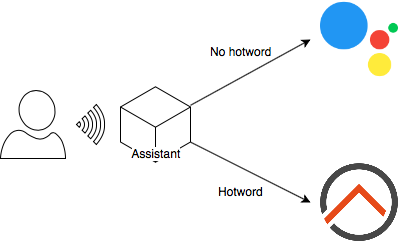
\includegraphics[width=0.65\textwidth]{images/Chapter_06/custom-assistant-simple.png}
	\caption{Basic diagram of the custom voice assistant}
	\label{fig:custom-assistant-simple}
\end{figure}

The previous script falls short for our purpose, as it does not include any integration with openHAB and it only triggers the 
assistant when the red button on the Google AIY box is pressed.

I worked over this example script, and some more that Google brings with this kit, in order to create a new one that integrates 
all the basic functionalities and works with openHAB. The main aspects to include are:
\begin{itemize}
    \item Activation via red button and “OK Google” command at the same time.
    \item Add custom commands to the assistant:
    \begin{itemize}
        \item Ability to manage openHAB from the assistant.
        \item Ability to manage the Raspberry Pi.
    \end{itemize}
    \item Possibility to integrate more languages.
\end{itemize}

\paragraph{Activating the Assistant via Voice Commands and by Pressing the Red Button}
I wanted users to be able to trigger the assistant in all the possible ways, so the first task is to make a script that can trigger 
the assistant by pressing the button and by saying “OK Google”.

We can make the program listen for “OK Google” by importing the Google Assistant Library. It will be listening on the microphone 
all the time waiting for this command, as any Android phone with Google Assistant would do. This library has direct access to the 
audio API, so our Python program does not need to record any audio.

However, the Google Assistant Library event loop (which is the responsible of hearing the “OK Google” command) blocks the running 
thread, so we cannot place everything in the same thread because the function that is executed when the button is pressed would 
never be invoked. We need to import threading and run the event loop in a separate thread.

To simplify matters, I will create a class called MyAssistant, which will create the threads in the constructor and will have a 
variable that will indicate if it is ready and an object of the Google Assistant.

\begin{lstlisting}[style=PythonCode]
class MyAssistant(object):

  def __init__(self):
      self._task = threading.Thread(target=self._run_task)
      self._can_start_conversation = False
      self._assistant = None

  def start(self):
      self._task.start()

  def _run_task(self):
      credentials = aiy.assistant.auth_helpers.get_assistant_credentials()
      model_id, device_id = aiy.assistant.device_helpers.get_ids(credentials)
      with Assistant(credentials, model_id) as assistant:
          self._assistant = assistant
          for event in assistant.start():
              self._process_event(event)

def _on_button_pressed(self):
if self._can_start_conversation:
          self._assistant.start_conversation()
\end{lstlisting}

This code snippet specifies just what we want to create at this moment. It has a call to the function \textit{\_process\_event()}, 
which will process our events. I will talk about it in the following sections.

\paragraph{Adding Custom Commands to the Assistant}
The Google Assistant responds to a huge variety of commands and can perform a considerable range of actions. Some devices even 
work with Google Home, but not many others that do work with openHAB 2. As we want to achieve an inexpensive, open-source home 
automation system, we need to integrate the assistant with openHAB 2, although this solution will also cover the devices that are 
compatible with Google Home, that are natively integrated with the assistant.

Unfortunately, we cannot customize Google Assistant commands, but we can build a basic assistant over this one that will cover our 
needs. Both will be working at the same time as well. 

I will use the Text-To-Speech engine that Raspbian integrates: \textit{pico2wave}. In the function \textit{\_process\_event()} that 
I mentioned before, we need to add some conditions for checking some “keywords” that will lead the program to stop the assistant 
for that command and execute our own one.

Apart from commands for managing openHAB 2, it is also a good idea to be able to manage the system from the assistant, as it is 
meant to be headless (that is, able to work without a screen connected) and powering off the Raspberry Pi by disconnecting the 
power cord is not recommendable. For now, I am going to add functions for powering off and rebooting the system:

\begin{lstlisting}[style=PythonCode]
def power_off_pi():
  aiy.audio.say('Powering off the system. Good bye!')
  subprocess.call('sudo shutdown now', shell=True)
	
def reboot_pi():
  aiy.audio.say('Rebooting the system. Hold on!')
  subprocess.call('sudo reboot', shell=True)
\end{lstlisting}

In each one, we define what the assistant is going to say when the function is executed with \textit{aiy.audio.say()} and what 
command to execute in the system with subprocess.call().

Then, with only one function we will be able to send any command to openHAB via REST. I have defined the URL in the same machine, 
as the Raspberry Pi is supposed to host the assistant and openHAB. The function creates a POST request that includes the item(s) 
and the desired state. When it gets the response, it responds with the success or failure of the command.


\chapter{Conclusions and future work}

Since the beginning of this project, the main objective has been maintained: to create an affordable, functional and usable voice-driven
home automation controller. At this point, we can tell that this objective has been mostly reached, although there are many things
to improve in a future.

When I began working on this system, I only knew some the most popular commercial virtual assistants with a home automation system,
like Google Home or Amazon Alexa, and none of them had been launched in the Spanish market. Today, almost ten months after, only
Google Home is available. It was when I started this project that I realized how many open source solutions were available, like openHAB.
This allowed me to work over an existing basis and to improve its capabilities, always maintaining the main objective of affordability
and functionality. The end result, although much less flexible, can offer most of the features offered by the main products on the
market. The custom voice assistant, that uses Google Assistant to answer all the commands not related to openHAB, makes this product
very useful for all kinds of situations.

One of the main issues that we have found is that this system needs to be configured by a technical person at least in its installation.
The installation of openHAB itself requires some technical knowledge, but its configuration and, most importantly, the configuration
of the voice assistant, requires coding. A very convenient future improvement would be to automate the generation of the voice
assistant script every time that a device is added. Of course, it would also be a good improvement to automate all the process.

This project relies heavily on third party solutions, like the Google services for processing the speech or the service
\textit{myopenHAB}. However, we have tried to explore and provide alternatives in every case, that would cover any different situation.

Another important future improvement is related to privacy. We observed that many devices, such as the Philips Hue Smart Bridge,
are in constant communication with the cloud, when in many cases this is not necessary. Some way of blocking this communication
and restricting it to the local network should be explored.

\begin{table}[]
	\centering
	\resizebox{\textwidth}{!}{%
		\begin{tabular}{|l|c|l|}
			\hline
			\multicolumn{1}{|c|}{\textbf{Objective}} & \textbf{Fulfillment} & \multicolumn{1}{c|}{\textbf{Observations}} \\ \hline
			\begin{tabular}[c]{@{}l@{}}1. Integrate a home automation \\ system in a embedded system\end{tabular} & 100\% & \begin{tabular}[c]{@{}l@{}}We have successfully installed and integrated\\ openHAB in the Raspberry Pi\end{tabular} \\ \hline
			\begin{tabular}[c]{@{}l@{}}2. Integrate a voice assistant in \\ the same embedded system as \\ the home automation system\end{tabular} & 100\% & \begin{tabular}[c]{@{}l@{}}The custom assistant integrates Google\\ Assistant and a voice assistant for\\ openHAB\end{tabular} \\ \hline
			\begin{tabular}[c]{@{}l@{}}3. Explore current home \\ automation systems and \\ voice assistants, focusing on \\ open-source solutions\end{tabular} & 80\% & \begin{tabular}[c]{@{}l@{}}We have explored some of these systems on\\ Chapter 3, but the inclusion of open source\\ solutions has been reduced\end{tabular} \\ \hline
			\begin{tabular}[c]{@{}l@{}}4. Explore automation \\ possibilities and implement\\ an automation service in the \\ domotic system\end{tabular} & 70\% & \begin{tabular}[c]{@{}l@{}}We have successfully implemented an \\ automation service using IFTTT and \\ the REST API of openHAB. Some other \\ services might have been explored\end{tabular} \\ \hline
			\begin{tabular}[c]{@{}l@{}}5. Explore options for \\ managing the system from a \\ mobile application\end{tabular} & 90\% & \begin{tabular}[c]{@{}l@{}}The system is currently manageable\\ thanks to the Cloud Connector and the\\ mobile application of openHAB\end{tabular} \\ \hline
			\begin{tabular}[c]{@{}l@{}}6. Explore options for \\ providing global access to the \\ system and implement one\end{tabular} & 100\% & \begin{tabular}[c]{@{}l@{}}We have explored these options on Chapter 6 \\ and we have tested the service \\ myopenHAB\end{tabular} \\ \hline
			\begin{tabular}[c]{@{}l@{}}7. Explore safety and privacy \\ concerns related to the home \\ automation system\end{tabular} & 30\% & \begin{tabular}[c]{@{}l@{}}Some safety concerns have been covered\\ through this work, but we have not covered\\ the main aspects related to privacy\end{tabular} \\ \hline
			\begin{tabular}[c]{@{}l@{}}8. Provide an adaptive and \\ responsive user interface, \\ usable on touch and non-touch \\ screens\end{tabular} & 100\% & \begin{tabular}[c]{@{}l@{}}We explained how to configure Basic UI and\\ PaperUI. Both user interfaces comply \\ with these points\end{tabular} \\ \hline
			\begin{tabular}[c]{@{}l@{}}9. Connect the virtual assistant\\ to the domotic system, so it can \\ manage the configured devices\end{tabular} & 100\% & \begin{tabular}[c]{@{}l@{}}The custom virtual assistant communicates\\ with openHAB thanks to the REST API\\ of openHAB and the Requests Python \\ library\end{tabular} \\ \hline
			\begin{tabular}[c]{@{}l@{}}10. Test domotic devices in the\\ final system and present an \\ usable solution\end{tabular} & 70\% & \begin{tabular}[c]{@{}l@{}}The current solution is completely\\ functional and usable. However, more \\ devices should have been tested\end{tabular} \\ \hline
		\end{tabular}%
	}
	\caption{Fulfillment of the specific objectives presented in Chapter 1}
	\label{table:fulfillment-objectives}
\end{table}

The table \ref{table:fulfillment-objectives} presents the fulfillment level of the specific objectives that we presented in the
Introduction chapter.


\nocite{asadullah16}
\nocite{openHABCommunity}
\nocite{raspberryPiForums}
\nocite{pythonDocumentation}
\nocite{mdnWebDocs}
\nocite{cmusphinxFaq}
\nocite{microsoftCortanaDev}
\nocite{cleveroad}
\nocite{jonesPythonCookbok}

\bibliographystyle{plain}
\bibliography{bibliography/bibliography}
\addcontentsline{toc}{chapter}{Bibliography}

\appendix
\chapter{Voice Assistant Script}

This appendix includes the full Python script of the voice assistant script that can communicate with Google Assistant and openHAB.

\begin{lstlisting}[style=PythonCode]
#!/usr/bin/env python3
# Copyright 2017 Google Inc.
#
# Licensed under the Apache License, Version 2.0 (the "License");
# you may not use this file except in compliance with the License.
# You may obtain a copy of the License at
#
#   http://www.apache.org/licenses/LICENSE-2.0
#
# Unless required by applicable law or agreed to in writing, software
# distributed under the License is distributed on an "AS IS" BASIS,
# WITHOUT WARRANTIES OR CONDITIONS OF ANY KIND, either express or
# implied.
# See the License for the specific language governing permissions and
# limitations under the License.

"""
Run a voice recognizer that uses the Google Assistant Library and TTS,
with customized commands for interacting with OpenHAB 2 via REST

The Google Assistant Library has direct access to the audio API, so this
Python code doesn't need to record audio.

Hot word detection "OK, Google" and button push are supported.

The Google Assistant Library can be installed with:
env/bin/pip install google-assistant-library==0.0.2

It is available for Raspberry Pi 2/3 only; Pi Zero is not supported.

Modified from Google AIY demo scripts by David Vargas
(https://github.com/dvcarrillo)
"""

import logging
import subprocess
import threading
import requests
import sys

import aiy.assistant.auth_helpers
import aiy.assistant.device_helpers
import aiy.audio
import aiy.voicehat
from google.assistant.library import Assistant
from google.assistant.library.event import EventType

# ---- CONFIGURATION ----
# openHAB server location
openhab_ip = "localhost"
openhab_port = "8080"

# Set the group containing all the lights
all_lights_group = 'Lights_ALL'

# Set the Items on OpenHAB related to your light bulbs
# The lights_ids array will be used for identifying each light in the
# spoken commands
light_colors = ['hue_0210_00178828e0d0_1_color']
light_color_temps = ['hue_0210_00178828e0d0_1_color_temperature']
lights_ids = ['office']     # Example: "turn on the office light"

# Hotwords that triggers the OpenHAB actions
custom_hotword = 'home'

# Show debug information (0 = false, 1 = true)
debug = 1
# -----------------------

# The en-GB voice is clearer than the default en-US
aiy.i18n.set_language_code('en-GB')

logging.basicConfig(
  level=logging.INFO,
  format="[%(asctime)s] %(levelname)s:%(name)s:%(message)s"
)

# -- OpenHAB 2 commands using OpenHAB REST API --

def openhab_send(item, state):
  url = 'http://' + openhab_ip + ':' + openhab_port + '/rest/items/' + item
  headers = { 'content-type': 'text/plain',
              'accept': 'application/json' }
  r = requests.post(url, headers=headers, data=state)

  if (debug):
    print('REQUEST [POST]: ' + url + ' STATE: ' + state)

  if r.status_code == 200:
    aiy.audio.say('OK')
  elif r.status_code == 400:
    if (debug):
      print('ERROR [HTTP 400]: ' + r.text)
    aiy.audio.say('There has been an error: bad command')
  elif r.status_code == 404:
    if (debug):
      print('ERROR [HTTP 404]: ' + r.text)
    aiy.audio.say('There has been an error: unknown item')
  else:
    aiy.audio.say('Command failed')

def openhab_get_state(item):
  url = 'http://' + openhab_ip + ':' + openhab_port + '/rest/items/' + item + '/state'
  r = requests.get(url)
  return r.text

# -- Power management commands --

def power_off_pi():
  aiy.audio.say('Powering off the system. Good bye!')
  subprocess.call('sudo shutdown now', shell=True)

def reboot_pi():
  aiy.audio.say('Rebooting the system. Hold on!')
  subprocess.call('sudo reboot', shell=True)

def not_recognized():
  aiy.audio.say('Sorry, I cannot do that yet')

def device_not_found():
  aiy.audio.say('Sorry, I don\'t know that device')

def test_speech():
  aiy.audio.say('Hello. This is a Text to Speech test.')

# -- Helper functions --

def any_idx(iterable):
  idx = 0
  for element in iterable:
    if element:
      return idx
    else:
      idx = idx + 1

# -- Class MyAssistant --

class MyAssistant(object):
  """
  An assistant that runs in the background.

  The Google Assistant Library event loop blocks the running thread entirely.
  To support the button trigger, we need to run the event loop in a separate
  thread. Otherwise, the on_button_pressed() method will never get a chance to
  be invoked.
  """
  def __init__(self):
    self._task = threading.Thread(target=self._run_task)
    self._can_start_conversation = False
    self._assistant = None

  def start(self):
    """
    Starts the assistant.

    Starts the assistant event loop and begin processing events.
    """
    self._task.start()

  def _run_task(self):
    credentials = aiy.assistant.auth_helpers.get_assistant_credentials()
    model_id, device_id = aiy.assistant.device_helpers.get_ids(credentials)
    with Assistant(credentials, model_id) as assistant:
      self._assistant = assistant
      for event in assistant.start():
        self._process_event(event)

  # State management and event processing
  def _process_event(self, event):
    status_ui = aiy.voicehat.get_status_ui()
    if event.type == EventType.ON_START_FINISHED:
      status_ui.status('ready')
      self._can_start_conversation = True
      # Start the voicehat button trigger.
      aiy.voicehat.get_button().on_press(self._on_button_pressed)
      if sys.stdout.isatty():
        print('\nSay "OK, Google" or press the button, then speak. '
          '\nTrigger the openHAB actions by saying \"' + custom_hotword +
          '\" at the beginning of each command.'
          '\nPress Ctrl+C to quit.\n')

      elif event.type == EventType.ON_CONVERSATION_TURN_STARTED:
        self._can_start_conversation = False
        status_ui.status('listening')

      elif event.type == EventType.ON_END_OF_UTTERANCE:
        status_ui.status('thinking')

      elif event.type == EventType.ON_RECOGNIZING_SPEECH_FINISHED and event.args:
        print('You said:', event.args['text'])
        text = event.args['text'].lower()

        # CHECK HOTWORD
        if text.startswith(custom_hotword):
          self._assistant.stop_conversation()
          text = text + " "

          # CHECK ACTION
          # Power, turn, set, change
          if any(token in text for token in (' turn ', ' power ', ' set ', ' change ')):
            # CHECK DEVICE
            # For all the lights
            if ' all ' in text and ' lights ' in text:
              if ' on ' in text:
                openhab_send(all_lights_group, 'ON')
              elif ' off ' in text:
                openhab_send(all_lights_group, 'OFF')
              else:
                not_recognized()

              # For a specific light
              elif ' light ' in text:
                # Get the index of the mentioned item in the light arrays
                idx = any_idx(token in text for token in lights_ids)
                if (idx != None):
                  direct_to_color = light_colors[idx]
                  direct_to_color_temp = light_color_temps[idx]
                  current_state = openhab_get_state(direct_to_color).split(',')

                  if ' on ' in text:
                    openhab_send(direct_to_color, 'ON')
                  elif ' off ' in text:
                    openhab_send(direct_to_color, 'OFF')
                  elif ' red ' in text:
                    new_state = "0,100," + current_state[2]
                    openhab_send(direct_to_color, new_state)
                  elif ' yellow ' in text:
                    new_state = "100,100," + current_state[2]
                    openhab_send(direct_to_color, new_state)
                  elif ' blue ' in text:
                    new_state = "260,100," + current_state[2]
                    openhab_send(direct_to_color, new_state)
                  elif ' pink ' in text:
                    new_state = "340,100," + current_state[2]
                    openhab_send(direct_to_color, new_state)
                  elif ' green ' in text:
                    new_state = "140,100," + current_state[2]
                    openhab_send(direct_to_color, new_state)
                  elif ' cool ' in text:
                    openhab_send(direct_to_color_temp, "0")
                  elif ' warm ' in text:
                    openhab_send(direct_to_color_temp, "100")
                  elif ' natural ' in text:
                    openhab_send(direct_to_color_temp, "50")
                  else:
                    not_recognized()
                else:
                  device_not_found()

              # For the system
              elif ' system ' in text:
                if ' off ' in text:
                  power_off_pi()
              else:
                not_recognized()

          # Increase, raise
          elif any(token in text for token in (' increase ', ' raise ')):
            if ' brightness ' in text and 'light' in text:
              idx = any_idx(token in text for token in lights_ids)
              if (idx != None):
                direct_to_color = light_colors[idx]
                current_state = openhab_get_state(direct_to_color).split(',')

                new_brightness = int(current_state[2]) + 25
                if (new_brightness > 100):
                    new_brightness = 100

                new_state = current_state[0] + ',' + current_state[1] + ',' + str(new_brightness)
                openhab_send(direct_to_color, new_state)
              else:
                device_not_found()
            else:
              not_recognized()

          # Decrease, reduce
          elif any(token in text for token in (' decrease ', ' reduce ')):
            if ' brightness ' in text and 'light' in text:
              idx = any_idx(token in text for token in lights_ids)
              if (idx != None):
                direct_to_color = light_colors[idx]
                current_state = openhab_get_state(direct_to_color).split(',')

                new_brightness = int(current_state[2]) - 25
                if (new_brightness < 0):
                    new_brightness = 0

                new_state = current_state[0] + ',' + current_state[1] + ',' + str(new_brightness)
                openhab_send(direct_to_color, new_state)
              else:
                device_not_found()
            else:
              not_recognized()

          # Reboot, restart
          elif any(token in text for token in (' reboot ', ' restart ')):
            if ' system ' in text:
              reboot_pi()
          else:
            not_recognized()

      elif event.type == EventType.ON_CONVERSATION_TURN_FINISHED:
        status_ui.status('ready')
        self._can_start_conversation = True

      elif event.type == EventType.ON_ASSISTANT_ERROR and event.args and event.args['is_fatal']:
        sys.exit(1)

  def _on_button_pressed(self):
    # Check if we can start a conversation. 'self._can_start_conversation'
    # is False when either:
    # 1. The assistant library is not yet ready; OR
    # 2. The assistant library is already in a conversation.
    if self._can_start_conversation:
      self._assistant.start_conversation()

def main():
  MyAssistant().start()

if __name__ == '__main__':
  main()
\end{lstlisting}


\newpage \
\thispagestyle{empty}

\end{document}
